%\documentclass[12pt,twoside]{report}
\documentclass[12pt]{report}

%% last modification is June 4, 2016, Emma Pease

% note that the document can be single or double sided.  
% note that the Registrar's office now allows 10pt, 11pt, or 12pt

\usepackage{suthesis}


\usepackage{amsmath}
\usepackage{amsthm}
\usepackage{amssymb}
\usepackage{mathrsfs}
\usepackage{stmaryrd}
\usepackage{graphicx}
 \usepackage{relsize}
 \usepackage{hyperref}
 \usepackage{tikz}
 \usepackage{colortbl}
\usepackage{color}
\definecolor{LightGray}{gray}{0.92}


%tables
\usepackage{tabularx}
\usepackage{array}
\usepackage{booktabs}
\usepackage{multirow}

\usepackage{gb4e}
\noautomath


\newcommand{\eref}[1]{(\ref{#1})}
\newcommand{\tableref}[1]{Table~\ref{#1}}
\newcommand{\figref}[1]{Figure~\ref{#1}}
\newcommand{\appref}[1]{Appendix~\ref{#1}}
\newcommand{\sectionref}[1]{Section~\ref{#1}}


\definecolor{PinkyPurple}{RGB}{178,0,178}
\newcommand{\todo}[1]{\textcolor{PinkyPurple}{\textbf{[TODO: #1]}}}

\renewcommand{\cite}[1]{[#1]}
\newcommand{\parencite}[1]{[#1]}


% default is now online June/2016 version
%\usepackage[online]{suthesis-2e}
%\usepackage[hardcopy]{suthesis-2e}
% the following is for doing engineering theses. 
% I am definitely not sure of the wording on the signature page so check
%\usepackage[engineer]{suthesis-2e}

% one can change the default font to Times Roman but note that most
% ways of creating pdf files from latex automatically embed (which btw
% is a good idea even with the standard fonts)

    \title{Semantic-pragmatic adaptation}
    \author{Sebastian Schuster}
    \dept{Linguistics}
    \principaladviser{Judith Degen}
    \firstreader{Christopher G. Potts}
    \secondreader{Daniel Lassiter}
%% one can also have a \thirdreader and \fourthreader

%% note that certain departments and types of theses have other requirements
%% For instance theses in the departments of 
%% Asian Languages
%% French and Italian
%% Spanish and Portuguese
%% need to define the \dept, \dualthesis, and the actual language
%\dualthesis
%\languagemajor{Chinese}
%% 
%% Those for Graduate Program in Humanities need to define 
%\humanitiesthesis
%\jointprogram{Arts and Crafts}
%% 
%% For submission to a committee or program (no department)
% \committeethesis
% \programthesis
%%
%% For School of Education or Business or Law
% \educationthesis
% \businessthesis
% \lawthesis  (law actually isn't listed in the official documents, 2013/1014)

\newcommand{\sem}[1]{\ensuremath{\llbracket#1\rrbracket}}

\begin{document}

% for a variety of reasons this is an all in one document; however,
% when actually doing the thesis it is strongly recommended that each
% chapter be in a separate file and use \include to include in the
% main file.

%% the \beforepreface command produces the title page
%% in the online version it skips the copyright (page 2) and signature (page 3) pages 
%% in the non-online version these would be included
    \beforepreface


%% Abstract can be any number of pages
    \prefacesection{Abstract}

    Speakers exhibit considerable production variability at all levels of linguistic representations. This raises the question how successful communication is nevertheless possible most of the time.
In this dissertation, I investigate this question and I study to what extent listeners adapt to variable use of words using the example of uncertainty expressions such as \textit{might} and \textit{probably}.  In several web-based experiments, I show that listeners exhibit uncertainty in their expectations about a generic speaker's use of uncertainty expressions;  that listeners update production expectations to match a specific speaker's use of uncertainty expressions after a brief exposure to that speaker; and that updated production expectations result in updated speaker-specific interpretations of uncertainty expressions. 

I further investigate the associated cognitive processes and I investigate what kind of representations listeners update during semantic-pragmatic adaptation. To this end, I  present a novel Bayesian computational model of production expectations of uncertainty expressions and a novel model of the adaptation process based on Bayesian belief updating.  Through a series of simulations, I find that post-adaptation behavior is best predicted by a model that assumes that listeners update both speaker-specific semantic representations and speaker-specific utterance choice preferences, suggesting that listeners update at least these two types of representations as a result of adaptation. 

Finally, I show in additional experiments that listeners adapt to multiple speakers and that adaptation behavior is modulated by non-linguistic contextual factors such as the speaker's mood. 

This work has implications for both semantic theories of uncertainty expressions and psycholinguistic theories of adaptation: it highlights the need for dynamic semantic representations and suggests that listeners integrate their general linguistic knowledge with speaker-specific experiences to arrive at more precise interpretations.





%% one can also have a prefacesection that is a Preface instead of
%% Acknowledgements.   The thematic purpose is the same (thanks).
    \prefacesection{Acknowledgements}
    Writing this dissertation (and surviving grad school) would have not been possible without the support of many people. My biggest thanks go to my advisor, Judith Degen, who has been the best mentor imaginable. Over the past three years, she has been a constant source of advice, support, encouragement, knowledge, wisdom, and inspiration. It's been incredibly fun working with her so closely on numerous projects, and I hope many more collaborations will follow!

Chris Manning took a leap of faith when he hired me as a research assistant midway through my master's without any serious experience in NLP research. Since then he taught me the basics of doing research and supported me along every step of my graduate career. Thank you for that (and many more things), Chris!

Chris Potts and Dan Lassiter taught my first two linguistics classes, and I am very grateful that years later both of them were part of my dissertation committee. Also thanks to Mike Frank and Tobi Gerstenberg for being on my defense committee. Thanks to Beth Levin for all the advice passed along while drinking tea in the linguistics kitchen, to Vera Gribanova for helping me get through the final stages of the PhD, and to Dan Jurafsky for being the most enthusiastic and kind chair that a linguistics department could have.

The computational linguistics and cognitive science communities at Stanford have been a great place to get inspired and to get feedback on (often half-baked) ideas. Thanks to all current and former members of the NLP group, and in particular to Abi See, Peng Qi, Kyle Mahowald, Jon Gauthier, Gabor Angeli, Spence Green, Siva Reddy, Sonal Gupta, Jesse Mu, and John Hewitt; to the members of the ALPS lab: Brandon Waldon, Daisy Leigh, Michael Hahn, Elisa Kreiss, Leyla Kursat, Eva Portelance, and Ciyang Qing; to Noah Goodman, Mike Frank, Eve Clark, Herb Clark, Tom Wasow, Michael Henry Tessler, and Robert Hawkins.

The linguistics department kitchen and the computational linguistics lab have been similarly great places for many discussions. Thanks to Prerna Nadathur, Simon Todd, Sara Kessler, Sunwoo Jeong, CJ Brickhouse, Emily Lake, and Zion Mengesha for the company at many Friday socials; and thanks to Rob Voigt, Tim Dozat, Dora Demszky, Ywei Luo, Matt Lamm, and Ignacio Cases for being wonderful office mates.

I couldn't have worked on many projects without wonderful collaborators: Masoud Jasbi, Natalia Silveira, Matthew Loder, Yuxing Chen, Sophie Regan, and Philip Weiss.

Grad school wouldn't have been the same without my cohort (and our joint trip to Tahoe): Reuben-Cohn Gordon, Daisy Leigh, Sabrina Grimberg, Branden Chan, and honorary cohort member Ed King.

I was also fortunate to meet many great linguists outside of Stanford. I had many great discussions that improved this dissertation with Chris Barker, Roger Levy, Michael Franke, Dave Kleinschmidt, Rachel Ryskin, Chigusa Kurumada, Sarah Moss, Ted Gibson, Greg Scontras, Molly Babel,  Emily Morgan, Tal Linzen, Greg Scontras, and Judith Tonhauser. And thanks to the entire Universal Dependencies community, and in particular to Marie-Catherine de Marneffe, Joakim Nivre, Miryam de Lhoneux, Teresa Lynn, and Djam\'e Seddah for many great collaborations.

Occasionally, I also did other things than research. Aaron Horvath and Katey Webber showed me the best bike routes around Stanford, Emily Carian (along with Eva Portelance and Christof Brandtner) proved that alphabetic constraints can make food even better, and Daisy Leigh and Ed King hosted the best parties on two continents. Thanks also to Max Hell and Natalie Johnson, Juan, Natasha, Miguel and Nico Pedroza, Jean Lin, Ece Kaynak, David Zuckerman, Matt Franklin, and Annie and Tyler Atura Bushnell for many joint adventures.

My parents, Johannes and Andrea, early on accepted my stubbornness to do things differently that eventually got me to Stanford. My siblings, Veronika, Magdalena, Karoline, and Valentin, are still among my closest friends and provided great excuses to frequently travel to Florida, Berlin, and Vienna. And my grandparents, Johann and Eva, made sure that I wasn't starving during my first year as a master's student.

Many friends in Vienna (and other places in Europe) made sure that I instantly felt at home whenever I visited the Old World: Ronald Malis, Markus Schmeiduch, Arthur Egger, Mona Wahba, Robert Pilgram, Niko Franjikic, Vivian Thiele-Orberg, Sabine Toifelhart, Pia Yazdanpanah, Gudrun Schweighofer, and Anna Wolf.

Eva Portelance joined me when I moved north to San Francisco two years ago. Together with her dog Dora, she created the most beautiful home I've ever lived in, instigated many formidable binge-watching sessions, got me a foster dog named Archie as a distraction from writing my dissertation, and was always there for me in one of the toughest years of my life.  Also, one day I hope to be half as good a cook as her.

From co-parenting Dark and Stormy to visiting the most beautiful places in the US to hosting pie parties, Christof Brandtner and later also Zenelia Paredes were there for almost all the greatest moments over the past eight years. Christof has a unique ability to create a community wherever he goes and my life in the US would not have been filled with as many great people without him.

Alessandra Peter has been the best travel companion, fellow raccoon enthusiast, and Vanillekipferl baking partner. She's also the best listener and nobody else could make me hike a trail in half of the recommended time or do pushups in a desert in Utah. I can't wait to explore New York together with her.

Finally, Markus Svoboda has been my best friend for almost two decades. Despite us not living in the same country for the past ten years, we're still in contact almost every day. He is an excellent mixer of G\&Ts and the best partner for rants about what the left is doing wrong. But even more importantly, he's been a constant pillar of support and always helps me put things in perspective. I dedicate this dissertation to him.



%% afterpreface produces a table of contents and any other tables
%% wanted. At the end pagenumbering changes from roman to arabic and
%% is restarted
    \afterpreface
 
%% Normally the \chapter and any text would be in a separate file and included.
    \chapter{Introduction}
    \section{Why adapt?}

* to know the meaning of words

* to draw the right implicatures

* go through example from cognition paper

\section{Defining the scope}

In this dissertation, I investigate the extent of semantic and pragmatic adaptation as well as
the associated cognitive processes. That is, to what extent do listeners learn speaker-specific
meanings of words; to what extent do listeners learn speaker-specific expectations of words,
and to what extent does this speaker-specific knowledge affect interpretations of utterances? 
And what are the cognitive processes that lead to this behavior?

In this enterprise, I focus on uncertainty expressions
such as \emph{might} and \emph{probably}. Thus, all findings will only directly apply to 
adaptation to variable use of uncertainty expressions. However, uncertainty expressions 
belong to the much larger class of context-sensitive expressions -- a class of expressions for 
which it is generally assumed  that their interpretation crucially depends on contextually 
specified parameters which -- as I will show in subsequent chapters --
are also tied to the speaker's identity. Given the extensive research on the parallels between
uncertainty expressions and other context-sensitive expressions such as quantifiers and
gradable adjectives \cite{LassiterBook, SchoellerFranke?}, the results in this dissertation
should therfore also apply to any other types of context-sensitive expressions, and all
the presented models could be easily extended to other classes of expressions. 

\section{Why uncertainty expressions?}

Uncertainty expressions have several properties that make them a good testing ground for studying semantic and pragmatic
adaptation. First, there is no consistent mapping between uncertainty expressions and event probabilities \cite{e.g., Clark1990,Pepper1974}, 
which suggests that listeners have to rely on additional contextual information (such as speaker identity)
if they want to infer an event probability that a speaker intended to communicate using an uncertainty expression. Second, there is considerable inter-speaker variability 
in the use of these expressions \cite{Wallsten1986} and therefore it is likely that listeners expect different speakers to use these expressions
differently. Lastly, interpreting uncertainty expressions plays an important role in many everyday situations from the banal -- 
such as talking about the weather -- to the serious -- such as communicating about health risks 
\cite{Berry2004, Lipkus2007, Politi2007} or making financial decisions \cite{Doupnik2003}. 
Thus, listeners would benefit from tracking  how a given speaker uses these expressions. 

\section{Structure of this dissertation}

main points of this dissertation:

* comprehension is an extremely flexible process 

* updated interpretations are guided by speaker expectations

* meaning of uncertainty expressions is flexible

* adaptation interacts in complex ways with other contextual factors (e.g., mood)



    \chapter{Background}
    \section{The semantics of uncertainty expressions}

While this is not a dissertation about modality, many of the utterances that I consider in my experiments contain an epistemic modal.
Since I discuss the implications of my experimental results for popular theories of the semantic of epistemic modals in Section~{XXX}, and since 
my computational model is inspired by recent accounts of epistemic modality, I provide a brief introduction to several theories of modality in this section.

Here, and throughout this dissertation, I adapt the broad notion of modality by \cite{Portner2009} and \cite{Kratzer2012Ch2}, which not only 
includes modal auxiliaries (e.g., \textit{might}, \textit{could}) but also other evidential devices such as probability operators 
(e.g., \textit{probably}) and attitude verbs (e.g., \textit{think}). At the same time, however, to limit the scope of this discussion,  
I will only cover epistemic modality, and therefore omit any discussion of deontic modals, i.e., modals to express how the 
world should be according to laws, societal norms, etc., which are frequently discussed together with epistemic modals.
I will also omit discussions of the important connections between modals and conditionals \cite{see e.g., Lewis1973?,Kratzer1978,Kratzer1979,Kratzer2012}
and discussions of the extent to which different semantic theories validate desired and undesired logical inferences \cite{see e.g., Yalcin2010}.

\subsection{Background: Possible world semantics}

Classical modal logic and most other semantic theories of modals are based on the concept of possible worlds \cite{kripke1963}.
A possible world is a world which differs in one or multiple properties from the actual world. For example, while the proposition $\phi_{brown}$
expressed by the  sentence ``I have brown hair'' is true in the actual world $w$, one possible world $w_1$ is identical in every regard to 
the actual world except that the proposition $\phi_{blond}$ encoded by ``I have blond hair'' is true and the one encoded by
``I have brown hair'' ($\phi_{brown}$) is false. 

According to  a possible world semantics, all sentences have to be evaluated relative to a possible world $w$ and
propositions $\phi$ can be represented as a set of worlds in which $\phi$ is true. If we consider the worlds $w$ and $w_1$ as described here,
the propositions expressed by the sentences ``I have brown hair'' and ``I have blond hair'' evaluate to different truth conditions, depending on the possible world.

$$\sem{\phi_{brown}}^w = 1 \mbox{ iff } w \in \phi_{brown}  = 1$$
$$\sem{\phi_{brown}}^{w_1} = 1 \mbox{ iff } w_1 \in \phi_{brown}  = 0$$
$$\sem{\phi_{blond}}^{w} = 1\mbox{ iff } w \in \phi_{blond} = 0$$
$$\sem{\phi_{blond}}^{w_1} = 1 \mbox{ iff } w_1 \in \phi_{blond} = 1$$




%* start off with why i'm talking about modals

%* what are modals

%* what are the questions relevant to modality

%* which ones of these are relevant for this thesis

%* Possible worlds

%* Modal logic

%* Kratzer

%* threshold semantics proposals

%* wallsten/budesco




%The semantics of epistemic modals\footnote{I adapt the broad notion of modality by \cite{Portner2009} and \cite{Kratzer2012}, which not only 
%includes modal auxiliaries (e.g., \textit{might}, \textit{could}) but also other evidential devices such as probability operators 
%(e.g., \textit{probably}) and attitude verbs (e.g., \textit{think}).} such as \textit{might}, \textit{could} and \textit{probably} 
%has been extensively discussed in the formal semantics literature. However, a lot of these works focus on how 
%different meaning representation affect logical inferences and how they can be used to compositionally derive the 
%meaning of sentences with modal expressions, which are less relevant debates for the enterprise in this dissertation.
%I therefore primarily give an overview of different formalisms along with a discussion about what they predict
%about the interpretation of epistemic modals when they are used to communicate probabilities of future events.

\subsection{Modal logic}

In classical modal logic, the truth conditions of sentences with epistemic modals depend on an accessibility relation $R$.
$R$ determines which worlds $w'$ are epistemically accessible from the actual world $w$, i.e., which worlds are epistemically consistent with
the actual world. For example, consider rolling two six-sided dice, one after another. Before you roll the first die, all worlds in which the sum of
the two dice is between 2 and 12 (all possible combinations of two dice) are epistemically accessible since they are compatible with the actual
world. Now, if you roll one of the dice and it comes up 4, only worlds in which the sum of the two dice is between 5 and 10 (all possible sums of 4 and 
a number between 1 and 6) are epistemically accessible. 

Formally, if $wRw'$ is true then $w'$ is epistemically accessible from $w$. A proposition $\phi$ embedded under an epistemic modal is then true
if either $\phi$ is  true in all epistemically accessible worlds (for necessity modals such as \textit{must}) or $\phi$ is true in at least one epistemically 
accessible world (for possibility modals such as \textit{might}).

\begin{exe}
\ex \label{ex:modall-must} $\sem{\mbox{must } \phi}^{w}  = 1 \mbox{ iff } \forall w' \in W: wRw' \rightarrow  \sem{\phi}^{w'} = 1$
\ex \label{ex:modall-might} $\sem{\mbox{might } \phi}^{w}  = 1 \mbox{ iff } \exists w' \in W: wRw' \rightarrow  \sem{\phi}^{w'} = 1$
\end{exe}

If we again use the example of rolling two dice and assume that the world $w_x$ corresponds to the sum 
of the two dice being $x$, then $wRw'$ is true iff $w' \in \{w_2, w_3, ..., w_{11}, w_{12}\}$. Therefore, for example,
\begin{align*}
\sem{&\mbox{must roll a number between 2 and 12}}^{w} =  1 \\
 & \mbox{(since \textit{roll a number between 2 and 12} is true in all epistemically accessible worlds)} \\ \\ 
 \sem{&\mbox{must roll a 7}}^{w} =  0 \\
 & \qquad \qquad \qquad \quad \mbox{ (since \textit{roll a 7} is only true in some epistemically accessible worlds)} \\ \\
 \sem{&\mbox{might roll a 7}}^{w} =  1 \\
 &  \qquad \qquad \qquad \qquad \quad \mbox{ (since \textit{roll a 7} is true in the epistemically accessible world }w_7\mbox{)}\\ \\ 
 \sem{&\mbox{might roll a 1}}^{w} =  0 \\
 &  \qquad \qquad \qquad \qquad \qquad \mbox{\  (since \textit{roll a 1} is false in all epistemically accessible worlds).}
\end{align*}

While this approach seems intuitively correct for scenarios like rolling two dice, it is very challenging to represent utterances
that convey more fine-grained meanings than mere possibility or necessity. As \cite{Lassiter2017} points out, one could extend this proposal
to modal expressions such as \textit{probably} and \textit{likely} by assuming that \textit{probably $\phi$} is true if $\phi$ is true in more 
epistemically accessible worlds than epistemically accessible worlds in which $\phi$ is false:
\begin{exe}
\ex $\sem{\mbox{probably} \phi}^{w}  = 1 $ \\ 
 \ \ \ \ \ \ \ \ $ \mbox{ iff } |\{w' \in W \mid wRw' = 1 \land \sem{\phi}^{w'} = 1\}| > |\{w' \in W \mid wRw' = 1 \land \sem{\phi}^{w'} = 0\}|$
\end{exe}
However, this proposal comes with at least two shortcomings if one wants to consider it as a 
complete theory of epistemic modals. First, one has to make the limit assumption \cite{Lewis1981}, i.e., 
one has to assume that $W$ contains a finite number of possible worlds. Second, this proposal does not provide 
a theory of interpretation for any type of graded epistemic modal expressions such as \textit{It is 60\% likely that...} or \textit{It is highly probable that...}
or modal expressions in comparative constructions such as \textit{It is twice as likely that X than Y} \cite{Lassiter2017}. Third, there
is no connection between event probabilities and the use of different modals except that this account would predict that \textit{might $\phi$} is true
when the probability of $\phi$ is greater than 0, and \textit{must $\phi$} is true if the probability of $\phi$ is 1.

%For my experiments, neither of this will be necessarily an issue; I am not dealing with graded expression 
%and the number of future events and hence also the number of possible world is limited. 
%However, two additional issues arise. First, given the previously established inter-subject variability in the interpretation 
%of epistemic modals \cite{Wallsten1986}, we need a theory that can accommodate variability. The only possibility to represent
%variability in this formalism would be to assume that either different speakers use different accessibility relations or different speakers
%use different sets of possible worlds. However, it seems unlikely that speakers who have access to the same kind of information 
%(the same visual stimuli both in \cite{Wallsten1986} and in my experiments) would rely on different accessibility relations or a different set of 
%possible worlds.

%Second, while intuitively this definition of \textit{probably} such that $\sem{\mbox{probably} \phi}^w$ is true if $\phi$ is more likely than $\lnot \phi$ 
%appears to be reasonable, there does not seem to be a similar definition for other uncertainty expression such as \textit{think} or \textit{looks like}.
%We could again assume that there are different accessibility relations associated with 

% and unless we assume
%variable accessibility relations $R$ or variable sets of possible worlds, this theory cannot represent 

% it remains unclear how this theory could predict any type of variability. Second, 



%probably $ wRw' and true / wRw' > 0.5$ 
%might $ wRw' and true / wRw' > 0$ 
%must $ wRw' and true / wRw' = 1$
%very likely $ wRw' and true / wRw' > 0.5 + \theta$
%more likely than $ wRw' and A is true / wRw' > wRw' and B is true / wRw'$

%issues: one has to be very careful how to set up the world structure --> otherwise law of probability no longer holds

%needs again limit assumption

%how is this better from just using probabilities?

\subsection{Double relativity of modals}

The most prominent semantic theory of epistemic modals (and all other flavors of modals) is the account by Kratzer 
\cite{Kratzer1981,1991}, later revised in \cite{Kratzer2012}. Building on \cite{Lewis1973}, she developed a unifying 
account of all modal flavors, which assumes that there are several core meanings of modals that can be expressed 
by various linguistic devices (e.g., \textit{could} and \textit{might} are both possibility modals), and that the interpretation
of a sentence with a modal depends on two \textit{conversational backgrounds}, that is, contextually specified functions 
from possible worlds to sets of propositions: 
the \textit{modal base} $f(w)$ and the \textit{ordering source} $g(w)$. 

The intuition behind the modal base $f(w)$ is that one can explicitly state which worlds the modal quantifies over using an 
``In the view of ...'' adverbial clause. For example, for epistemic modals, the modal base may be a function that returns the set of propositions
that are compatible with what is knowns in the current world, which can be explicitly expressed in a sentence with an epistemic modal through the
adverbial clause ``In the view of what is known'':

\begin{exe}
\ex In the view of what is known, it could rain tomorrow.
\end{exe}

\noindent Kratzer argues that utterances without explicit mention of a conversational background are interpreted
by contextually resolving the relevant modal base. If we ignore the ordering source for a second, this leads to the following 
definitions of $f$-necessity and $f$-possibility.

\begin{quote}
\noindent $f$-\textit{necessity}: \\
$\phi$ is a necessity with respect to a modal base $f$ iff $\phi \subseteq \cap f(w)$.

\noindent $f$-\textit{possibility}: \\
$\phi$ is a possibility with respect to a modal base $f$ iff $\cap \{\{\phi\} \cup  f(w) \} \ne \emptyset$.
\end{quote}

The semantics of sentences with necessity modals such as \textit{must} and possibility modals such as \textit{might}
can then be expressed in terms of $f$-necessity and -possibility:

\begin{exe}
\ex $\sem{\mbox{must }\phi}^{w,f} = 1 \mbox{ iff $\phi$ is an $f$-necessity in $w$} $
\ex $\sem{\mbox{might } \phi}^{w,f} = 1 \mbox{ iff $\phi$ is an $f$-possibility in $w$} $
\end{exe}

The semantics of these expressions is equivalent to the classical modal logic semantics presented in (\ref{ex:modall-must})  and (\ref{ex:modall-might}), 
since the accessibility relation $R$ can be defined as $wRw' = w' \in \cap f(w)$. For this reason, this account suffers from the same
issues as the classical modal logic account: it cannot be used to derive interpretations for graded modals or comparatives.

Kratzer partially resolves these issues by introducing a second conversational background, 
the ordering source $g(w)$. $g(w)$ defines a partial preorder $\le_{g(w)}$ over the set of possible worlds $W$ such that 
$$u \le_{g(w)} v \mbox{ iff } \{ p \in g(w) \mid u \in p \} \subseteq \{ p \in g(w) \mid v \in p \}.$$
That means, $v$ is at least as close to an ideal as $u$ iff all propositions in the set of ideal 
propositions $g(w)$ that are true in $u$ are also true in $v$. In the case of epistemic modals, 
the ideal as defined by $g(w)$, is usually assumed to contain propositions corresponding to a normal course of events.

Necessity and possibility then be defined as follows.
\begin{quote}
\noindent \textit{Necessity}: \\
$\phi$ is a necessity with respect to a modal base $f$ and an ordering source $g$ iff for all $u \in \cap f(w)$, there is a $v \in \cap f(w)$
such that $u \ge_{g(w)} v$ and for all $z \in \cap f(w):$ if $v \ge_{g(w)} z$, then $z \in \phi$.

\noindent \textit{Possibility}: \\
$\phi$ is a possibility with respect to a modal base $f$ and an ordering source $g$ iff $\lnot \phi$ is not a necessity with respect to $f$ and $g$.
\end{quote}
\noindent Intuitively, the definition of necessity can be seen as further restricting the modal source such that something must be true if it is true in 
all epistemically accessible worlds that come closest to the ideal defined by the ordering source. 

To illustrate how the modal base and the ordering source work together, imagine a murder case in a small town in which 
there are four suspects A, B, C, and D who all have a motive.\footnote{Example adapted from \cite{Kratzer2012Ch2}.} Further,
there was a tourist T from Iceland in town when the murder happened. Since random tourists rarely murder somebody without
a motive, the set of normal propositions $g(w)$ in this example could be $\{a, b, c, d\}$, where each proposition corresponds to
 A, B, C, and D committing the murder, respectively. 
However, the conversational background of what is known $f(w)$ is compatible with A, B, C, D, or T being the murderer,
i.e., $\cap f(w) = \cup \{a, b, c, d, t\}$. Now, it seems natural for a police officer to utter (\ref{ex:kratzer-a-murder-might})
or  (\ref{ex:kratzer-abcd-murder-must}) but unlikely for the officer to utter (\ref{ex:kratzer-t-murder-might}).

\begin{exe}
\ex \label{ex:kratzer-a-murder-might} A might have committed the murder.
\ex \label{ex:kratzer-abcd-murder-must} A or B or C or D must have committed the murder.
\ex \label{ex:kratzer-t-murder-might} T might have committed the murder.
\end{exe}

\noindent Kratzer's account makes exactly these predictions. It predicts that (\ref{ex:kratzer-a-murder-might}) is true because 
$\lnot a$ is not a necessity and therefore $a$ is a possbility; it predicts that (\ref{ex:kratzer-abcd-murder-must}) since 
$a \lor b \lor c \lor d$ is a necessity; and it  predicts that (\ref{ex:kratzer-t-murder-might}) is false since $\lnot t = a \lor b \lor c \lor d$ is a necessity
and therefore $t$ is not a possibility.

Apart from introducing this distinction between normal courses of events and theoretically possible courses of events, Kratzer's account also
provides a semantics for comparatives using the notion of comparative possibility.\footnote{This is the revised definition of comparative possibility from
in \cite{Kratzer2012Ch2} which is slightly different from the original notion of comparative possibility in \cite{Kratzer1981}.}
\begin{quote}
\noindent \textit{Comparative possibility}: \\
$\phi$ is at least as good a possibility as $\psi$ in $w$ with respect to a modal base $f$ and an ordering source $g$ iff 
$$\lnot \exists u ( u \in \cap f(w) \land u \in \phi-\psi \land \forall v (( v \in \cap f(w) \land v \in \psi-\phi) \rightarrow v <_{g(w)} u))$$
\end{quote}
\noindent	Further, $\phi$ is a better possibility than $\psi$ iff $\phi$ is at least as good a  possibility as $\psi$ and $\psi$ is 
not at least as good as possibility as $\phi$. Using this definition, \cite{Kratzer1991} defines the semantics of \textit{probably} as
\begin{exe}
\ex $\sem{\mbox{probably } \phi}^{w,f,g}  = 1 \mbox{ iff $\phi$ is a better possibility than $\lnot \phi$}.$ 
\end{exe}
\noindent Similarly, the semantics of \textit{$\phi$ is more likely than $\psi$} can be defined as 
\begin{exe}
\ex $\sem{\phi \mbox{ is more likely than } \psi}^{w,f,g}  = 1 \mbox{ iff $\phi$ is a better possibility than $\psi$}.$ 
\end{exe}	

As compared to classical modal logic, this proposal has the advantage of providing a semantics for comparative constructions and
a semantics for \textit{probably}. However, this account still does not provide a compositional account for modal expressions and 
therefore does not provide a semantics for expressions such as \textit{very likely}. Second, this account also does not make predictions
about the use of epistemic modals to communicate and infer event probabilities. \cite{Kratzer2012} briefly discusses event probabilities and shows that one
can come up with probability measures on the set of sets of possible worlds $\mathcal{P}(W)$ such that $\phi \ge_{g(w)} \psi$ implies $P(\phi) \ge P(\psi)$. 
However, her discussion does not go beyond showing that a connection between event probabilities and possible worlds is possible and 
her semantic account of modals leaves it open how speakers and listeners map modals to event probabilities.

\subsection{Threshold semantics}

in recent years, there have been several proposals for an alternative semantics of epistemic modals based on the idea that the meaning of 
epistemic modals is determined by the position of the probability of the embedded proposition on a probability scale
\cite{e.g., Swanson2006,Yalcin2010,Lassiter2017}. The truth condition of utterances with epistemic modals is then determined by whether
the probability of the embedded proposition exceeds some threshold $\theta_x$ associated with the modal $x$:

\begin{exe}
\ex $\sem{\mbox{must }\phi}^{w} = 1 \mbox{ iff $P(\phi) > \theta_{must}$ in $w$} $
\ex $\sem{\mbox{might } \phi}^{w} = 11 \mbox{ iff $P(\phi) > \theta_{might}$ in $w$} $
\ex $\sem{\mbox{probably } \phi}^{w} = 11 \mbox{ iff $P(\phi) > \theta_{probably}$ in $w$} $
\end{exe}

This account is inspired by accounts of gradable adjectives \cite{e.g., Kennedy2007} and the observation that many 
epistemic modals are likely gradable adjectives. For example, \cite{Lassiter2017} argues that \textit{possible}, \textit{probable},
\textit{likely}, and even \textit{certain} all behave in many regards like gradable adjectives: Similarly to gradable adjectives like \textit{tall}, 
they can be used with degree modifiers  (\ref{ex:degree-mod}), and measure phrases (\ref{ex:measure-phrase}), and they can be part of comparative clauses (\ref{ex:comp-clause}).

\begin{exe}
\ex \label{ex:degree-mod} \begin{xlist}
\ex Joan is \textbf{very} tall.
\ex It is \textbf{very} probable that you'll win the lottery.
\end{xlist}
\ex \label{ex:measure-phrase} \begin{xlist}
\ex Joan is \textbf{6ft} tall.
\ex It is \textbf{70\%} likely that you'll win the lottery.
\end{xlist}
\ex  \label{ex:comp-clause}  \begin{xlist}
\ex Joan is tall\textbf{er} than Bob.
\ex That you'll get hit by lightning is \textbf{more} likely than that you'll win the lottery.
\end{xlist}
\end{exe}

\noindent Because of this parallelism, threshold accounts, which have been successfully used to represent the meaning of gradable adjectives,
can also be straightforwardly applied to graded or comparative epistemic modals. For example, the utterances in \ref{ex:degree-mod}b), 
\ref{ex:measure-phrase}b), and (\ref{ex:comp-clause}b)
can be represented as follows.

\begin{exe}
\ex $\sem{\mbox{very probable } \phi}^w = 1 \mbox{ iff $P(\phi) \gg \theta_{probable}$ in $w$}$
\ex$ \sem{\mbox{70\% likely } \phi}^w = 1 \mbox{ iff $P(\phi) = .7$  in $w$}$
 \ex$ \sem{\phi \mbox{ more likely than } \psi}^w = 1 \mbox{ iff $P(\phi) > P(\psi) $  in $w$}$
\end{exe}

As the choice of examples in this section indicates, the arguments for this account are primarily
based on observations concerning epistemic adjectives. Whereas the modal logic account and Kratzer's
account focus on the meaning of epistemic auxiliaries and much less on observations concerning
epistemic adjectives and adverbs, threshold accounts put epistemic adjectives and adverbs front and center
and treat auxiliaries more as an afterthought. Given that auxiliaries are generally not gradable, it
might appear surprising to assume a threshold semantics for auxiliaries. However, beyond the fact
that a unified account leads to a simpler theory, there is also the argument that 
epistemic adjectives and auxiliaries can be used in the same 
utterance to strengthen the meaning.

\begin{exe}
\ex You might win the lottery but you probably won't.
\end{exe}

\noindent It would be strange to assume that \textit{probably} in this utterance expresses
that the probability of not winning the lottery exceeds some threshold but that \textit{might}
does not make any reference to an event probability.

One other question this account raises, is how to set the thresholds. For modals such as \textit{probably} that describe
event probabilities that are clearly not at either end of the probability space, there is agreement that the threshold is
to at least a certain extent context-dependent. For example, in the case of a coin flip with two possible outcomes
the threshold will most likely be above .5.

\begin{exe}
\ex The coin will probably land on tails.
\end{exe}

\noindent It would be unexpected for a speaker to produce this utterance if the probability of the coin landing on tails was actually
below .5 and it would be more likely for the coin to land on heads. However, when there are more outcomes, the threshold can be lower.
For example, \cite{Teigen1988} asked participants 10 days before the 1986 Eurovision Song Contest finals to estimate the chances of winning for 
20 contestants using the responses \textit{probable}, \textit{not probable}, and \textit{neither probable nor improbable}.  He found that no subject
used \textit{probable} only once, which -- given that participants could have only assigned a winning probability of more than .5 to at most one of the contestants --
indicates that participants also endorsed the statement for event probabilities less than .5. In part, this result was likely driven by the very limited response options
in this forced choice production experiment but later work has also found that participants use different uncertainty expressions to describe an event depending on the
alternative outcomes and that, for example, likely is sometimes also used to describe event probabilities lower than .5 \cite{e.g.,  WindshitlandWells1998}.
%\footnote{Note though that unlike what \cite{Yalcin2010} claims, \cite{WindshitlandWells1998} never ran an acceptability study of  statements like ``Bloggs is probably the winner..."}

For auxiliaries, on the other hand, there is less agreement about whether the threshold should be context-sensitive. \cite{Yalcin2010} argues
for a probabilistic version of existential and universal quantifications such that the thresholds for \textit{might} and \textit{must} are 0 and 1, respectively.
\cite{Swanson2006}, on the other hand,  argues for \textit{might} and \textit{must} being duals, that is that the threshold for \textit{might}, $\theta_{might}$, 
and the threshold for \textit{must}, $\theta_{must}$, both depend on a single parameter $\mu$ such that  $\theta_{might} = \mu$ and  $\theta_{must} = 1 - \mu$. 
He further argues for a weak interpretation of epistemic must that implies a threshold below 1, and consequently a $\mu > 0$, which in return also implies
that  \textit{might} is only true for probabilities greater than $\theta_{might} = \mu > 0$. Based on data from truth value judgement tasks, \cite{Lassiter2017} 
more generally argues that the thresholds for \textit{might} and \textit{must} are context-sensitive and generally greater than 0 and smaller than 1, respectively. 
He also considers \textit{might} and \textit{must} as being duals and takes the result that participants sometimes rejected statements with \textit{might} for very low
event probabilities as evidence for the possibility of \textit{might} using a threshold greater than 0 and for \textit{must} having a weak interpetation.
In summary, there exist three proposals for the thresholds of epistemic auxiliaries: a) treating \textit{might} and \textit{must} as duals and assuming a strong interpretation
of \textit{must} \cite{Yalcin2010}; b) treating them as duals and assuming a weak interpretation of \textit{must} \cite{Swanson2006}, and c) treating \textit{might} and
\textit{must} as duals and assuming context-sensitive thresholds \cite{Lassiter2017}. I will discuss this issue in much more detail in the subsequent chapters.

Finally, we can again ask whether this representation can predict how language users map event probabilities to uncertainty expressions.
This account is based on probabilities and therefore does make predictions about this mapping. However, given that uncertainty expressions
only have a lower bound, this theory by itself does not predict why a speaker would produce \textit{probably} instead of \textit{might} when there is
a high event probability, or why a speaker would produce \textit{certainly} instead of \textit{possibly} when the event probability is 1, since
in either case both expressions are true. As has been demonstrated by \cite{HerbstrittandFranke2019} and as I will also show in the next chapter, this
issue can be easily reconciled by adding a pragmatic machinery on top of a threshold semantics that predicts that speakers will prefer more informative
utterances. 

To conclude this section, while the question of how thresholds should be set has not been fully settled, this account has -- unlike the two previous accounts that i presented 
--  the advantage of directly linking event probabilities to uncertainty expressions and being able to make predictions about ranges of event probabilities for which different
uncertainty expressions can be used.

\section{Verbal probability expressions}

In a line of work that has largely operated in parallel to modality research, there has also been considerable research 
into how uncertainty expressions or -- as they are referred to in this literature -- verbal probability expressions are used
to communicate probabiklities of future events. The overarching goals of this line of work have been to determine how
language users map uncertainty expressions to probabilities and how probabilities communicated through uncertainty expressions
shape decision behavior \cite{BudescuWallsten1995}. 

Initially, this field operated under the assumption that there exists a conventional mapping between uncertainty expressions
and probabilities and several works tried to develop methods intended for probing this mapping. For example, \cite{BethMarom1982} 
tried to infer single point probabilities associated with various uncertainty expressions; \cite{Hamm1991} tried to elicit which ranges of
probabilities uncertainty expressions map to; and \cite{WallstenBudescuRapoportetal.1986} tried to infer membership functions, i.e., 
functions that assign a value from 0 to 1 to each probability indicating how exemplary for an uncertainty expression a given
event probability is. Membership functions are a concept from fuzzy logic and are therefore distinct from probability distributions but 
 membership functions and probability density functions are homomorphous, so one can think of them as representing how likely a 
probability is communicated by a given uncertainty expression.

While \cite{WallstenBudescuRapoportetal1986} successfully managed to infer membership functions of uncertainty expressions
that largely remained constant for individual participants across multiple experimental sessions, they also found that there is considerable
inter-subject variability, suggesting that the mapping varies considerably across individual language users and challenging
the assumption of a conventional mapping. \cite{WallstenBudescuRapoportetal1986} only speculated about the reasons 
for this variability but they assumed that this variability was caused by individual differences such as different educational backgrounds
or different experience levels with uncertainty expressions.

The finding that there exists considerable variability inspired a lot of follow-up work to identify contextual factors
affecting interpretations and productions of uncertainty expressions. These factors include base probability events (e.g.,
\textit{probable} describing the likelihood of snow in the North Carolina mountains in December is interpreted to describe
higher event probabilities than when describing the probability of snow in October \cite{WallstenFillenbaumandCox1986}); 
outcome severity (more severe consequences lead to inferring higher probabilities \cite{WeberHilton1990}); outcome valence
(positive events lead to higher inferred probabilities \cite{MulletRivet1991}); and the alternatives presented in the experiment 
\cite{Filenbaumetal1991}.

Despite this progress in identifying contextual factors, there has not been progress in modeling how contextual factors
affect the interpretation of uncertainty expressions nor has there been much work on identifying systematicity in
inter-speaker variability. Instead, \cite{Budescuetal2009} declared defeat and argued that uncertainty expressions
lead to an ``illusion of communication'' because they are so vague that speakers and listeners employ different meanings
without being aware of these differences (see also \cite{AmerHackenbrackNelson1994,BrunTeigen1998,TeigenBrun1999}).
 \cite{Budescuetal2009} therefore changed their focus to studying how to best present probabilities in texts as to avoid the illusion 
 of communication. I will argue in subsequent chapters that declaring complete defeat has been premature. While I do not question
 that there are communicative scenarios in which speakers and listeners employ different meanings and therefore
 fail to communicate event probabilities properly, I will argue that there are scenarios in which listeners readily update speaker
 expectations and interpretations of uncertainty expressions, suggesting that accurate communication can be achieved in many
 scenarios through adaptation.
  
 % I will argue (similarly to \cite{CollinsandHahn2018}) that this complete declaration of defeat has been premature, and that
 %at least in part several aspects of the experimental setups can be attributed to the seemingly unavoidable illusion 

Setting aside the issue of variability for a moment, we can also ask whether membership functions could be a suitable 
meaning representation for uncertainty expressions. Membership functions -- unlike accounts based on possible worlds --
are capable of making predictions about the use of uncertainty expressions to communicate event probabilities, so prima facie
they appear to be a good candidate for a meaning representation. However, one challenge for this account is the fact that
according to most experimentally inferred membership functions, the meaning of uncertainty expressions is both lower-bounded and upper-bounded,
i.e., according to this account an uncertainty expression can only be used if the probability that one wants to communicate is above a certain lower 
bound $\alpha$ and below a certain upper bound $\beta$. For example, if we assume that the membership function of \textit{might} assigns
non-zero values to probabilities in the interval $[ 0.1,0.5 ]$, then a speaker can only use \textit{might} to communicate event probabilities above 
$\alpha=.1$ and  below $\beta=.5$. This upper-boundedness then leads to contradictions if the scalar inference from \textit{might} to a stronger 
alternative such as \textit{certainly} is explicitly canceled, as in (\ref{ex:might-impl-canceled}), and the membership functions of the two 
uncertainty expressions do not overlap.
\begin{exe}
\ex \label{ex:might-impl-canceled} You might get a scholarship, in fact you certainly will. 
\end{exe}   
This utterance communicates an event probability $p$ such that $\alpha_{\mbox{might}} \le p \le \beta_{\mbox{might}}$ and 
$\alpha_{\mbox{certainly}} \le p \le \beta_{\mbox{certainly}}$ which does not exist if the membership functions of these two expressions
do not overlap and  $\beta_{\mbox{might}}$  is lower than $\alpha_{\mbox{certaintly}}$, leading to a contradiction. This indicates that while
membership functions are possibly a good representation for the use of uncertainty expressions in many contexts, they are not well-suited
as a proper semantic representation. 



\section{The Rational Speech Act framework}

The Rational Speech Act (RSA; \cite{GoodmanFrank2016}, see also \cite{FrankeJaeger2016}) framework provides a computational-level
theory of how speakers choose utterances from a set of alternative utterances and how listeners interpret utterances. The framework is
a game-theoretic probabilistic formalization of Gricean \cite{Grice1975} pragmatic reasoning and casts interpretation of utterances as probabilistic Bayesian
inference, following recent successes in Bayesian modeling of many cognitive processes (e.g., \cite{TenenbaumGrowingAMind}). 

According to an RSA model, two types of agents engage in a communicate game: speaker agents $S$ and listener agents $L$. The goal of a speaker agent is to communicate
a world state $w$ from a set of possible worlds $W$ to a listener by choosing an utterance $u$ from a set of alternative utterances $U$; the goal of the listener agent is to infer the world 
state $w$ after hearing the utterance $u$. Speaker agents and listener agents reason about each other when choosing and interpreting utterances, leading to a
recursive probabilistic reasoning process. Generally, as a base case of this recursive process, the lowest level is represented by a so-called literal listener $L_0$.\footnote{
\todo{mention cases in which $S_0$ is the base case.}}
The literal listener interprets an utterance probabilistically according to a semantic interpretation function $\sem{\cdot}$ of the utterance, 
resulting in a distribution over world states $w$ given an utterance $u$.\footnote{To keep the definitions compact, I omit the normalization terms from all definitions here. 
Note, however, that all listener and speaker distributions are probability distributions and therefore always have to be normalized to sum to 1.}
$$L_0(w \mid u) \propto P(w) \times 
\begin{cases}
1 & \mbox{if } w \in \sem{u} \\
0 & \mbox{otherwise} 
\end{cases}$$
The literal listener $L_0$ thus chooses a world state at random from all the worlds in which $u$ is true (as returned by $\sem{u}$).

A pragmatic speaker agent $S_1$ then reasons about this literal listener when choosing their utterance. The formal goal of the 
pragmatic speaker is to soft-maximize \cite{Luce1959,Sutton1998} the speaker utility $U(w,u)$, which balances how informative the utterances is to $L_0$ and
how costly $u$ is to produce, as indicated by the cost function $c(u)$. Informativity is defined as the negative log surprisal of $L_0$, resulting
in the following utility function $U$ and speaker distribution $S_1$.
$$U(w,u) = \log L_0(w \mid u) - c(u)$$
$$S_1(u \mid w) \propto \mbox{exp} \left( \lambda U(w,u) \right)$$
$\lambda$ is a rationality (or temperature) parameter guiding how likely a speaker is to choose the optimal utterance. 
Speaker choices are rational if $\lambda > 0$ and choices become increasingly optimal as $\lambda$ approaches $\infty$.

\begin{figure}
\center
\includegraphics[width=.5\textwidth]{plots/faces-ad-hoc-implicature.png}
\caption{\label{fig:faces-ad-hoc-imp}: Referents in ad-hoc implicature reference game.}
\end{figure}

At the next level, pragmatic listeners $L_1$ try to infer the world state that the speaker intended to communicate
through Bayesian inference: $L_1$ integrates their prior beliefs about the state of the world $P(w)$ with the likelihood
of the speaker $S_1$ choosing the observed utterance to communicate $w$:
$$L_1(w \mid u) \propto P(w) \times S_1(u \mid w)$$

This recursive reasoning process can theoretically be continued ad infinitum by adding additional speaker and listener agents that 
reason about their respective counterpart agents one level below $i-1$ the current level $i$:
$$U_i(w,u) = \log L_{i}(w \mid u) - c(u)$$
$$S_i \propto \mbox{exp} \left( \lambda U_{i-1}(w,u) \right)$$
$$ L_i(u \mid w) \propto P(w) \times S_i(u \mid w)$$

\todo{mention IBR}

In practice, however, this recursive process is usually capped at the $L_1$ and $L_2$ level (\todo{add reference. Franke and Degen?}) and the models
that I will consider in this dissertation are also all capped at the $L_1$ level.



This recursive reasoning process implicitly models a Gricean counterfactual reasoning process in which listeners reason about alternative utterances
that a speaker could have produced but didn't to interrpret To illustrate how this works, consider a simple reference game as shown in Figure~\ref{fig:faces-ad-hoc-imp}.\footnote{Example adapted from \cite{GoodmanFrank2016}.} In this game,
there are three faces: one without any accessories (\textbf{n}), one with glasses (\textbf{g}), and one with glasses and a hat (\textbf{gh}). A speaker chooses one of the three faces
and tries to communicate her choice to the listener through an utterance $u$. In this contrived example, let us assume that the only three possible utterances that the
speaker can choose from are $U=\{\mbox{\textsc{face}: My friend has a face},\mbox{\textsc{glasses}: My friend has glasses},$ $\mbox{\textsc{hat}: My friend has a hat}\}$, 
and that the listener is aware that the speaker can only choose from these three utterances. Speakers tend to show the following behavior in this game. If they refer
to \textbf{n}, they produce \textsc{face}, if they refer to \textbf{g}  they produce \textsc{glasses}, and if they refer to \textbf{gh} they produce \textsc{hat}. Conversely, listeners infer that 
the speaker likely referred to \textbf{n} after hearing \textsc{face}, to \textbf{g}  after hearing \textsc{glasses}, and to \textbf{gh} after hearing \textsc{hat}.

An RSA model rooted at a literal listener $L_0$ with a pragmatic speaker $S_1$ and a pragmatic listener $L_1$ captures this behavior. In this game, 
the semantic interpretation function $\sem{\cdot}$ is defined as:

\begin{center}
\begin{tabular}{c | c } 
$u$ & \sem{u} \\ \midrule
\textsc{face} & $\{\mathbf{n}, \mathbf{g} , \mathbf{gh}\}$  \\
\textsc{glasses} & $\{ \mathbf{g} , \mathbf{gh}\}$ \\
\textsc{hat} &$\{\mathbf{gh}\}$ \\
\end{tabular}
\end{center}

\noindent Computing the distributions for $L_0 (w\mid u)$ -- if we assume uniform priors over the three referents -- then results in:

\begin{center}
\begin{tabular}{c | c | c | c} 
$u$ & $L_0( \mathbf{n} \mid u)$ &  $L_0( \mathbf{g} \mid u)$ &  $L_0( \mathbf{gh} \mid u)$ \\ \midrule
\textsc{face} & $\frac{1}{3}$ & $\frac{1}{3}$ & $\frac{1}{3}$  \\
\textsc{glasses} &0  & $\frac{1}{2}$ & $\frac{1}{2}$  \\
\textsc{hat} & 0 & 0 & 1 \\
\end{tabular}
\end{center}

\noindent At the two extremes, $L_0$ thus chooses a face at random after hearing \textsc{face}, which is true about all three 
faces but it will always choose \textbf{gh} after hearing \textsc{hat}, which is only true for \textbf{gh}. As I mentioned above, the
pragmatic speaker $S_1$ then chooses an utterance by soft-maximizing their utility, which depends on the informativity of $u$
to communicate $w$ to $L_0$ and the cost $c(u)$, which I assume to be 0 for all utterances in this example. If we further assume
that the rationality parameter $\lambda=1$, then $S_1(u \mid w)$ is:

\begin{center}
\begin{tabular}{c | c | c | c} 
$w$ & $S_1( \textsc{face} \mid w)$ &  $S_1( \textsc{glasses} \mid w)$ &  $S_1( \textsc{hat} \mid w)$ \\ \midrule
\textbf{n} & 1  & 0 & 0  \\
\textbf{g} &$\frac{2}{5}$  & $\frac{3}{5}$ & 0  \\
\textbf{gh} & $\frac{2}{11}$ & $\frac{3}{11}$ & $\frac{6}{11}$ \\
\end{tabular}
\end{center}

\noindent This speaker model qualitatively predicts the behavioral data from forced choice production experiments \cite{GoodmanFrank2016}: for all three
referents the most likely utterance choice according to $S_1$ matches the most likely choice in the experimental data. However, this behavior could have
also been predicted by purely symbolic counterfactual reasoning processes as outlined in \cite{Grice1975, Hirschberg1989}. The real advantage of this model 
comes from the fact that it is a quantitative model and if one fits the rationality parameter $\lambda$ to the experimental data, one can also quantitatively predict 
utterance choices in a population of participants.

Finally, the pragmatic listener $L_1(w \mid u)$ can be used to predict the interpretation of utterances in this context. If we again assume that the prior over referents $P(w)$
is uniform, $L_1$ is:

\begin{center}
\begin{tabular}{c | c | c | c} 
$u$ & $L_1( \mathbf{n} \mid u)$ &  $L_1( \mathbf{g} \mid u)$ &  $L_1( \mathbf{gh} \mid u)$ \\ \midrule
\textsc{face} & $\frac{55}{87}$ & $\frac{22}{87}$ & $\frac{10}{87}$  \\
\textsc{glasses} &0  & $\frac{11}{16}$ & $\frac{5}{16}$  \\
\textsc{hat} & 0 & 0 & 1 \\
\end{tabular}
\end{center}

\noindent This listener model qualitatively predicts the behavioral data from the interpretation experiments, and once again one can quantitatively predict participants' proportions
of choosing the three referents after hearing a given utterance by fitting the rationality parameter $\lambda$. 

Predicting utterance choices and interpretations in this contrived example of an ad-hoc implicature may not seem particularly impressive. However, many subsequent works
following the original RSA model have extended this basic model to predict a wide range of pragmatic phenomena, including predicting scalar inferences 
\cite{GoodmanStuhlmuehller2013}, embedded implicatures \cite{Potts2016}, M-implicatures \cite{Bergen2016}, metaphors and hyperbole \cite{Kao2013,Kao2014,Kao2015}, 
irony \cite{Kao,CohnGordon2019}, the use of gradable adjectives \cite{LassiterGoddman2015, QingFranke2014}, generics \cite{Tessler2019}, vague quantifiers 
\cite{SchoellerFranke2017}, politeness \cite{Yoon2019}, social meaning\cite{Burnett2017}, and -- as I will discuss in more detail in the next chapter -- 
to predict the use and interpretations of epistemic modals \cite{HerbstrittFranke2019}. While almost all of these models 
introduce additional extensions to the model as presented here, they crucially all rely on the recursive Bayesian reasoning process outlined in this section,
highlighting the versatility of models that cast pragmatic behavior as an instance of Bayesian reasoning.







    \chapter{Production expectations}
    \section{Experiment 1: Pre-exposure ratings}
\label{sec:exp-norming}

We first conducted a norming study, which served the following theoretical and methodological purposes.
First, it served as a methodological check on whether the paradigm is suited for 
manipulating fine-grained event probabilities. 
Second, it addressed the theoretical question of whether listeners vary in their expectations about
a generic speaker's use of uncertainty expressions, by collecting participants' judgments about 
uncertainty expressions they expected speakers to use for varying probabilities of receiving gumballs of a particular color from a gumball machine. 
Third,  the results from this study informed the experimental design of the adaptation experiments 
reported in later sections, by allowing us to both choose which pair of uncertainty expressions to test adaptation on, 
and to determine the particular event probability for which participants had roughly equi-probable expectations 
about which expression of uncertainty a generic speaker would use to report an event with that probability. 
Lastly, we used the data collected in this study to 
estimate population-level prior beliefs for the adaptation model reported in Section 5.

\subsection{Method}

\subsubsection{Participants}
We recruited a total of 420 participants 
(20 per condition) on Amazon Mechanical Turk. 
We required participants to have a US-based IP address and a minimal approval rating of 95\%.
Participants were paid \$1.80 (condition 1), \$1.50 (conditions 2-15),
or \$2.00 (conditions 16-21),
depending on the number of trials,
which amounted to an hourly wage of approximately \$12--\$15. 


% Figure 2: plots/fig-2-pre-test-example-trial.jpg (one column figure)
\begin{figure}[th!]
\center
\includegraphics[width=0.7\textwidth, trim={0 0 1.1cm 0},clip]{plots/fig-2-pre-test-example-trial.jpg} 
\caption{Example trial in Experiment~1. \label{fig:norming-trial} }
\end{figure}

\subsubsection{Materials and Procedure}
This study was a production expectation experiment intended to probe listeners' expectations about a generic speaker's language use.
Participants were instructed that over the course of the experiment, they would see several scenes with an adult man, 
a young girl, and a gumball machine on a table and 
that the gumball machine is too high up on the table for the girl to see (see Figure~\ref{fig:norming-trial} for an example scene). 
After completing an attention check which asked participants whether 
the girl could see the gumball machine,\footnote{Participants had to go back to the instructions in case they responded incorrectly. This was the case for 41 participants.} 
participants saw a series of scenes  and were asked to rate how likely they thought it was that the 
adult would produce two given responses by distributing 100 points across the two given utterances and the 
blanket \textit{something else} option (\textsc{other}). Sliders automatically jumped back if participants tried to distribute more than 100 points. 
In each scene, the child uttered \textit{``I want a blue one''} (target color: blue) or  \textit{``I want an orange one''} (target color: orange), randomized across participants.\footnote{In condition 1 (\textit{bare-might}), as well as conditions 16-21 (all conditions with \textit{bare not}), the target color was randomized across trials. While randomization of the target color across trials increased the correlation between the ratings for the two colors,  the average ratings for each condition independent of the target color were not affected by this choice. See Appendix A or a detailed discussion of the effect of this manipulation on the ratings.} The gumballs in the machines were tossed around continuously to prevent participants from counting the gumballs
and to make sure that participants did not consider it more likely to get one of the gumballs at the bottom of the machine.
 In each of the 21 conditions, participants saw only  two of the following seven possible adult utterances with different uncertainty expressions:\footnote{In the choice of the investigated expressions, we follow recent work on the interpretation of uncertainty expressions \cite{Pogue2018} and aim to use naturalistic utterances. We therefore decided against using a frame such as \emph{``It is UNCERTAINTY-ADJ that''} that would have fixed the syntactic structure across items because such a frame would have resulted in less naturalistic expressions like  \emph{``It is possible that''} or  \emph{``It is probable that''}, which are much less common than the expressions we considered (e.g., \textit{might} appears more than 30 times more often than \textit{possible that} in the spoken portion of the Contemporary American English \cite{Davies2009}). A speaker's use of these rare expressions thus could have triggered additional pragmatic inferences due to violations of the maxim of manner \cite{Grice1975} that are unrelated to our research questions.}

 \begin{itemize}
\item You'll get a blue/orange one. (\textsc{bare}\footnote{As a notational convention, we refer to utterances with uncertainty expressions in \textsc{small caps} and to the uncertainty expression itself in \textit{italics}. })
\item You might get a blue/orange one. (\textsc{might})
\item You'll probably get a blue/orange one. (\textsc{probably})
\item I think you'll get a blue/orange one. (\textsc{think})
\item It looks like you'll get a blue/orange one. (\textsc{looks like})
\item You could get a blue/orange one. (\textsc{could})
\item You won't get a blue/orange one. (\textsc{bare not})
\end{itemize}


\noindent Within each condition, we manipulated the percentage of target color gumballs across trials, which we take as proxy for the objective probability of receiving a gumball of the target color. 
Each participant saw 3 trials\footnote{In condition 1 (\textit{bare-might}), participants saw each gumball machine 6 times: 3 times when being asked to produce a statement about orange gumballs and 3 times when being asked to produce a statement about blue gumballs. In conditions 15-20 (all conditions with \textit{bare not}), participants saw each machine 4 times: 2 times for each color.} 
for each of the following percentages: 0\%, 10\%, 25\%, 40\%, 50\%, 60\%, 75\%, 90\%, 100\%. We randomized the order of expressions across participants and trials were presented in randomized order.

\subsection{Results and Discussion}

% Figure 3: plots/fig-3-pre_test_main.pdf (2-column figure)
\begin{figure}
\includegraphics[width=\textwidth]{plots/fig-3-pre\string_test\string_main.pdf} 
\caption{Results from 3 conditions of Experiment~1. Error bars correspond to bootstrapped 95\%-confidence intervals. \label{fig:norming-results-main} }
\end{figure}

Figure~\ref{fig:norming-results-main} shows participants' ratings for different gumball proportions for 3 of the 21 conditions, namely all combinations of the conditions
with the utterances \textsc{bare}, \textsc{probably}, and \textsc{might} (see Appendix~B for the results from the other 18 conditions). 
The results from these three conditions highlight several important properties of participants'
behavior in this experiment that generalize to all conditions.
First, the ratings for individual utterances are influenced by the utterance choices presented to participants.
If we compare the ratings for \textsc{might} in the \textit{bare-might} and the \textit{might-probably} condition, we see that \textsc{might} received high ratings for a larger
range of event probabilities when it is paired with \textsc{bare} than when it is paired with \textsc{probably}. We observe similar effects for the other two utterances.
This suggests that participants are cued towards using the utterances provided in the experiment and that their ratings depend on the presented alternatives -- an effect that
has also been observed for frequency expressions \cite{Chase1969} and quantifiers \cite{Degen2016}.

Second, the results suggest that participants are sensitive to the different event probabilities and that this paradigm is well suited to study 
the mapping between event probabilities and uncertainty expressions. For example, in the \textit{might-probably} condition, participants
provided considerably different ratings when they were presented with a gumball machine with 50\% target color gumballs than when they
were presented with 60\% target color gumballs.


% Figure 4: plots/fig-4-pre_test_main_indiv.pdf (2-column figure)
\begin{figure}
\includegraphics[width=\textwidth]{plots/fig-4-pre\string_test\string_main\string_indiv.pdf}
\caption{Results of three individual participants in the \emph{might-probably} condition of the Experiment~1. \label{fig:norming-results-indiv}}
\end{figure}


Third, in all conditions, the mean ratings are graded and except for the 0\% and 100\% target color gumball trials, the average rating for none of the
utterances is close to 100. There are two potential explanations for this observation. It could be that participants provided categorical ratings, i.e.,
generally assigned 100 points to one of the three options but the category boundaries vary across participants which leads to the graded average ratings.
It could also be that participants' individual ratings are graded which could reflect participants' uncertainty about which utterance a speaker would use 
and that these individual graded ratings drive the  graded average ratings. If we look at individual participants' ratings, it appears to be a combination of both.
Figure~\ref{fig:norming-results-indiv} shows the responses of three individual participants in the \emph{might-probably} condition. These figures show that there 
is a range of gumball proportions for each participant for which they assigned similar ratings to two utterances, which suggests uncertainty about the speaker's 
utterance choice. At the same time, however, this range also differed across participants: Participant \#8, who considered the experimental speaker a 
``\textit{cautious}'' speaker, thought that the speaker would only be likely to use {\sc probably} 
when the objective probability of getting a target color gumball was greater than 0.75, whereas participant \#15, who considered the experimental speaker a `
`\textit{confident}'' speaker, thought that  {\sc probably} was a better utterance choice than {\sc might} 
when the objective probability of getting a target color gumball was just greater than 0.5. These observations suggest that for some event probabilities, participants have uncertainty  about a 
speaker's choice of uncertainty expression and that participants have a priori different expectations about how a generic speaker would use these expressions.

This uncertainty and variability seems to be particularly borne out in the \emph{might-probably} condition. For this reason, we chose this pair of expressions
to study listeners' adaptation to variable uses of uncertainty expressions.

\subsubsection{Aside: The effect of the question under discussion}

One potential issue with the experimental design is that participants could consider additional speaker goals
beyond being informative. For example, given that the speaker is talking to a child, it could be that participants
assume that he wants to be particularly encouraging and the the choice of his expressions is shaped by both informative
and social goals \cite{Yoon2019}. To investigate whether this is the case, I therefore conducted additional exploratory experiments with
the \emph{might-probably} expression pair in which I manipulated the question under discussion \cite{QUD; Robers1996} by manipulating 
the utterance produced by the girl. In the \textsc{preference} condition, the speech bubble read \emph{``I want a blue/an orange one''} as in the experiment
above. In the \textsc{dispreference} condition, the speech bubble instead read ``\emph{I \textbf{don't} want a blue/an orange one''}, indicating
a dispreference by the girl for the color under discussion. In the \textsc{disjunction} condition, the speech bubble read 
\emph{``Will I get a blue or an orange one?}'', indicating no preference for one or the other color. 

If participants only consider informativity as a goal, there should be no effect of the QUD and the ratings in the 
\textsc{dispreference} and \textsc{dijsunction} conditions should be identical to the ratings 
in the \textsc{preference} condition. However, if participants expect the speaker to be particularly encouraging in the 
conditions in which the girl expresses a preference or dispreference for one color, we would expect different
ratings depending on the QUD.\footnote{One could imagine the effect going in either direction. It could be that
participants expect the speaker to be particularly encouraging and therefore expect the speaker to use 
the stronger uncertainty expression \textit{probably} for lower event probabilities in the \textsc{preference} condition than 
in the \textsc{dispreference} condition. On the other hand, it could be that participants expect the speaker to be scared 
of disappointing the child and therefore expect him to use \textit{probably} for higher event probabilities in the \textsc{preference} 
condition than in the \textsc{dispreference} condition.} If the child's preference affects ratings, the ratings in the  
\textsc{disjunction} condition should lie between the other two versions of the experiment.

\paragraph{Methods.} I recruited 40 participants (20 per version) on Amazon Mechanical Turk. 
The requirements were the same as in the original experiment and none of the participants 
participated in the original experiment. Participants were paid  \$2.50.

The procedure was identical as in conditions 16-21 in the previous experiment and participants
completed 36 trials. Across conditions, I manipulated the QUD by changing the utterance in
the speech bubble above the child:
\begin{itemize}
\item I want a blue/an orange one (\textsc{preference} condition)
\item I don't want a blue/an orange one  (\textsc{dispreference} condition)
\item Will I get a blue or an orange one? (\textsc{disjunction} condition)
\end{itemize}

\begin{figure}
\includegraphics[width=\textwidth]{plots/pre-test-qud.pdf}
\caption{Mean ratings for each uncertainty expression with different questions under discussion. Error bars correspond to bootstrapped 95\%-confidence intervals. \label{fig:norning-qud}}
\end{figure}


\paragraph{Results and discussion.} \figref{fig:norning-qud} shows the ratings for the three conditions grouped by uncertainty expression. Overall, the ratings
are very similar across conditions and there are no significant differences between conditions, except that the rating for \emph{probably} is significantly
higher in the \textsc{preference} condition than in the \textsc{dispreference} condition when there is a 100\% event probability, and the reverse is true for
the \emph{other} utterance. The main takeaway from this experiment is therefore that the QUD has at most very little impact on speaker expectations in
this paradigm. 

That being said, it is noteworthy that the numerical differences are very systematic and suggest subtle effects of the QUD on speaker expectations. First,
unrelated to any social goals, I found that in the 10-50\% event probability range, participants in the \textsc{disjunction} condition consistently rated \textsc{might}
 lower than in the other two conditions, and they rated the \emph{other} utterances higher. A likely explanation for this observation is that participants find it more natural to respond with a statement
involving the more frequent color if they child asks \emph{``Will I get a blue or an orange one?}''.  Therefore participants consider  it less likely that the speaker
would respond with \emph{``You might get a blue one''} if there is a very low probability of getting a blue gumball. (Recall that the response options always included
only one color term; in the \textsc{preference} and \textsc{dispreference} conditions, the color in the response options was the same as in the child's 
utterance but in the \textsc{disjunction} condition, the color in the response options was counterbalanced across trials.) In the other two conditions, the color term
was part of the QUD and therefore participants find it more likely that the speaker would respond with \textsc{might}.

The second noteworthy difference is that on the 100\% event probability trials, \textsc{probably} is rated lower in the \textsc{dispreference} condition
than in the other two conditions. A possible explanation for this observation is that participants believe that the speaker would try harder to avoid 
the scalar inference from \textit{probably} to \textit{not certainly} when the outcome is less desired based on the following reasoning:
 If the child infers from the use of \textit{probably} that it is not certain that she will get the undesired gumball, she might be somewhat hopeful
 that she could still get the desired gumball and will be more disappointed when she inevitably gets the undesired gumball. While this explanation
 is highly speculative, it is consistent with findings that social goals influence interpretations and expectations about productions of expressions
 that may give rise to scalar inferences \cite{Bonnefon, Yoon2019}.
 
 To sum up this aside, these exploratory experimental results suggest that the QUD affects production expectations but importantly only to a very small
 extent. For this reason, I continue to use the child's request \emph{``I want a blue/an orange one''} in the subsequent adaptation studies, assuming that
 in this paradigm, social goals have a negligible impact on participants' expectations.


 





\section{Modeling expectations about uncertainty expression productions}
\label{sec:model-baseline}

In this section we propose a computational model of expectations about uncertainty expression production that is informed by the data from Experiment 1. This model will serve as proxy for listeners' baseline generative model of a generic speaker and will be used as the basis for investigating adaptation processes in \sectionref{sec:model-adapt}. Experiment~1 confirmed previous findings that participants' expectations 
about how a generic speaker would use uncertainty expressions 
depend on the set of utterances that participants can choose from.
We further found that ratings were graded in part because participants had uncertainty about how a generic speaker would use uncertainty expressions. 
Hence, a model that accounts for participants' beliefs about a speaker's production of uncertainty expressions
 should  (a) be able to capture differences in ratings depending on the availability of alternative utterances;
(b) provide graded predictions about utterance probabilities; 
and (c) be able to capture within-participant uncertainty about probability of use.

Computational game-theoretic models such as the Rational Speech Act 
framework (RSA; \cite{Goodman2016})  are uniquely suited to satisfy the above desiderata.
RSA models are a probabilistic formalization of Gricean pragmatics which model comprehension as Bayesian probabilistic inference. 
They consist of \textit{listener} and \textit{speaker} agents which recursively reason about each other to derive interpretations and choose utterances. 
For our purposes of modeling production expectations, we focus on a model of listener beliefs about a speaker's production model.
  According to  RSA, a {speaker} that wants to
 convey some information to a {listener}
chooses an utterance based on the utterance's utility compared to the utility of alternative utterances. 
The {speaker}'s utterance utility is determined by trading off the informativity of the utterance to a \textit{literal listener} on the one hand and the cost of the utterance on the other.

In defining the informativity of an utterance, we follow previous RSA models of uncertainty expressions (\cite{Herbstritt2019}) 
and assume that uncertainty expressions have a threshold semantics \cite{Swanson2006,Yalcin2010,Lassiter2016}. That is, for each uncertainty expression $e$ there exists some threshold $\theta_e \in [0,1]$ 
such that an utterance $u_e$ with $e$ is true if the probability $\phi$ 
of the proposition embedded under $e$ exceeds $\theta_e$. 
For example, if we assume the threshold for \textit{might}, $\theta_{might}$, is 0.1, then the statement 
``It might rain this afternoon'' is semantically available to a {speaker} who believes that the probability of rain in the afternoon exceeds $0.1$.
Formally, we base the computation of informativity on a probability distribution from utterances to event probabilities $\phi$, 
which is usually referred to as the \textit{literal listener} $L_0$ in the RSA framework. 

$$L_0\left(\phi \mid u_e, \theta_e\right) \propto P(\phi) \times 
\begin{cases}
1 & \mbox{if } \phi > \theta_e\\
0 & \mbox{otherwise} 
\end{cases} \qquad \mbox{(for positive embedded propositions)}$$
$$L_0\left(\phi \mid u_e, \theta_e^{'}\right) \propto P(\phi) \times 
\begin{cases}
1 & \mbox{if } \phi < \theta_e^{'} \\
0 & \mbox{otherwise} 
\end{cases} \qquad \mbox{(for negated embedded propositions)}$$

According to this formalization, the {literal listener}  randomly draws an event probability $\phi$ from all values above  the threshold $\theta_e$ associated with the uncertainty expression $e$ (or, in the case of negated propositions, from all values below the threshold $\theta_e^{'}$). $P(\phi)$ is a prior distribution over event probabilities, which is independent of the observed utterance.

A \textit{pragmatic speaker} $S_1$ that intends to communicate an event probability $\phi$ then chooses an utterance $u_e$ with uncertainty expression $e$ from a set of utterances $U$ according to a soft-max choice rule \cite{Luce1959,Sutton1998} such that $u$ is chosen with a probability proportional to the utility for the speaker:
$$S_1\left(u_e \mid \phi, \theta, c\right) \propto exp \left( \lambda \left( \log L_0\left(\phi \mid u_e, \theta_e\right)  - c(u_e)\right)\right)$$
$\lambda$ is a rationality parameter which governs how likely the {speaker} is to choose the utterance that maximizes utility. As $\lambda$ approaches infinity, the {speaker} is more likely to always choose the optimal utterance. As it approaches 0, the {speaker} produces true utterances at random.\footnote{
The absolute value of this parameter is influenced by the literal listener distributions and the cost function. It is therefore complex to determine a reasonable range for $\lambda$ a priori, except that the value should be greater than 0 for the agent to not behave irrationally.} 

% Figure 5: plots/fig-5a-model-visualization-distributions.pdf and plots/fig-5b-model-visualization-predictions.pdf (1.5-column figure)
\begin{figure}[th!]
\includegraphics[width=\textwidth]{plots/fig-5a-model-visualization-distributions.pdf}

\includegraphics[width=\textwidth]{plots/fig-5b-model-visualization-predictions.pdf}

\caption{Example threshold distributions (upper panels) and corresponding model predictions for the \textit{expected pragmatic speaker} model (lower panels). In this example, the set of possible utterances is $U=\{$\textsc{bare}, \textsc{might}, \textsc{probably}, \textsc{bare not}$\}$, all utterances have equal costs, the rationality parameter $\lambda$ is set to 10, and the prior probability over event probabilities $P(\phi)$ is a uniform distribution. As the panels on the left show, point estimates of thresholds lead to sharp categorical boundaries in the model predictions, whereas distributions over thresholds, as in the panels on the right, lead to gradually increasing and decreasing predicted utterance ratings. \label{fig:model-visualization}}
\end{figure}

$S_1$ crucially depends on a vector of thresholds $\theta$ which contains a threshold for each uncertainty expression in the utterances in $U$, 
as well as a cost function $c(u)$. The values that participants expect a \textit{pragmatic speaker} to assign 
to these variables are unknown a priori; we infer these values from the data collected in the above reported experiment. 
In Experiment~1, we found that both at the population level and at the individual level, 
participants' ratings of the different expressions gradually increased and decreased with changing event probabilities 
(as, for example, shown in Figure~\ref{fig:norming-results-indiv}). This is expected if participants
have probabilistic beliefs about thresholds $\theta$ (as illustrated in the right panels of Figure~\ref{fig:model-visualization}) but not if they reason based on point estimates of $\theta$ (as illustrated in the left panels of Figure~\ref{fig:model-visualization}).
Considering these observations,  we assume that listeners hold beliefs about a speaker's thresholds in the form of a distribution $P\left(\theta_e\right)$.\footnote{We leave it open 
whether a {speaker} samples from a distribution over thresholds when producing utterances (as suggested by \cite{Qing2015}) 
or always uses the same values for thresholds. In the former case, listeners could have higher-order beliefs  $P(\eta)$ 
about different {speakers}' threshold distributions instead of having direct beliefs about the thresholds that different 
{speakers} use. For our purposes, this distinction does not matter since we assume that listeners would marginalize over higher-order beliefs $P(\eta)$ such that  $P\left(\theta_e\right) = \int P\left(\eta\right) P\left(\theta_e \mid \eta\right) d\eta$ and we therefore take the simplest approach and directly model $P\left(\theta_e\right)$. } Analogously, we assume that  listeners also have beliefs $P(c)$ about the speaker model's cost function.
Using these two distributions, we can define the \textit{expected pragmatic speaker} model $ES_1\left(u_e \mid \phi \right)$ as follows:

$$ES_1\left(u_e \mid \phi \right) = \int P(c) \int_0^1 P(\theta) S_1\left(u _e\mid \phi, \theta, c\right) d\theta \  d c$$

This model predicts which utterance listeners with uncertainty about a speaker's thresholds and cost function would expect that {speaker} to use to describe different event probabilities. 
Intuitively, this model can be seen as a weighted average of different \textit{pragmatic speaker} models, where individual models differ in terms of thresholds and cost functions.  The weights of this average are determined by listeners' belief distributions over thresholds and costs. For example, if listeners believe that it is likely that a speaker uses a threshold $\theta_{probably}$ of 0.5, they will assign higher weight to speaker models
using this threshold than models using other thresholds. 

\subsection{Linking function}

We assume that in Experiment~1, participants, when asked to provide ratings for utterances, reasoned about a generic speaker's 
likely descriptions of varying event probabilities. 
We assume that this reasoning was guided by participants' beliefs about the speaker's thresholds and costs, and 
that participants averaged over their uncertainty. For this reason, we assume that the population-level 
average ratings of what participants expect the speaker to say in different situations 
correspond to the probabilities predicted by the \textit{expected pragmatic speaker} model (with the \textit{something else}
option being predicted by the sum of the probabilities of all utterances not present in a condition; see below for more details).
Further, given the forced choice nature of the experiment and that we estimate model 
parameters from limited and potentially noisy data, we make the following additional linking assumptions
for which we provide a rationale and an assessment of their importance in turn.

\begin{itemize}
\item \textbf{Set of utterances}: Across all conditions, we assume that the set of utterances that participants are 
considering is the set of all utterances that we used in Experiment~1, i.e., $U= \{$ \textsc{bare}, \textsc{might}, 
\textsc{probably}, \textsc{think}, \textsc{looks like}, \textsc{could}, \textsc{bare not}$\}$. We include all utterances 
instead of only the utterances that are presented in a given condition since we assume that participants' general 
knowledge of English uncertainty expressions also influences their ratings. Ideally, we would include even more 
utterances in this set of alternatives but since we can only estimate parameters for uncertainty expressions for 
which we collected ratings, we are limited to the utterances in $U$. 

The exact set of utterances has only a small impact on the model's predictions as long as the set includes the \textsc{bare}
and \textsc{bare not} utterances as well as at least one utterance with a weaker 
(e.g., \textit{might}) and one with a stronger (e.g., \textit{probably})
uncertainty expression. If this requirement is met, the model makes the same qualitative predictions, 
and closely matches the quantitative predictions of a model that includes all 7 utterances choices.

\item \textbf{\textit{something else} option}: Participants in condition $\mathscr{C} = \{u_a, u_b\}$ 
could only choose between the three utterances $U' = \{u_a, u_b,$ \textit{something else}$\}$.
For modeling data from condition $\mathscr{C}$, we therefore need a function to predict the ratings 
for the utterances in $U'$. For $u_a$ and $u_b$, this is straightforward: We assume the probability 
of a participant choosing $u_a$ or $u_b$
is proportional to $ES_1(u_a \mid \phi)$ and $ES_1(u_b \mid \phi)$, respectively. 
We model the probability of a participant choosing the \textit{something else} option as the sum 
of the probability of all utterances that were not part of the condition as well as a constant $O$, 
which accounts for probability mass assigned to utterances that participants might be 
considering but which are not contained in $U$. This gives us the following condition-specific 
function $ES_1^{(\mathscr{C})}$ for predicting participants' ratings.

$$
ES_1^{(\mathscr{C})}(u \mid \phi) \propto 
    \begin{cases}
      ES_1(u \mid \phi) & \quad\mbox{if } u  \in \mathscr{C}\\
       O + \sum_{u \not \in \mathscr{C}} ES_1(u \mid \phi) & \quad \mbox{if $u$ is \textit{something else}} \\
   \end{cases}
$$

This summation over alternative utterances is crucial for fitting the data since we need to
capture the ratings for \textit{something else}. The only viable alternative would be
to fit individual curves for \textit{something else} for each condition, which would require
the estimation of considerably more parameters and would not explain the ratings for the
\textit{something else} option. The inclusion of the constant $O$ is less important but it
still improves model fit.


\item \textbf{Cost function}: We assume that the cost function represents participants' beliefs about the speaker's 
preferences for different utterances. Lower costs of an utterance indicate higher speaker preferences. We further 
assume that we are cueing participants to believe that the speaker would be likely to use the two utterances, $u_a$ 
and $u_b$, that are provided in condition $\mathscr{C}=\{u_a, u_b\}$ and that participants therefore primarily use the 
\textit{something else} option when both of the two utterances are semantically infelicitous or otherwise highly unexpected. 
We model this cueing effect in our choice of the cost function $c(u)$, which depends on the condition. For the two utterances 
that are presented to the participants, we set the cost to $1$ and for all the other utterances, we set the cost to a constant $\gamma > 1$:
$$
c(u, \mathscr{C}) = 
     \begin{cases}
       1 &\quad\text{if } u  \in \mathscr{C}\\
       \gamma &\quad\text{otherwise} \\
     \end{cases}
$$

Theoretically, we could have also used a different constant $\gamma_u$ for each utterance. The data from
Experiment~1, however, suggests that participants generally did not prefer one utterance over 
the other. To limit the number of free model parameters and to prevent overfitting, we therefore use a single
constant $\gamma$ for all utterances. We will, however, relax this assumption in our adaptation model in \sectionref{sec:model-adapt}, which
we use to investigate whether listeners update their beliefs about preferences during adaptation.

This condition-specific cost function is important for the model fit. If we didn't use such a cost function, 
the model would assign much higher ratings to the \textit{something else} option than participants did.

\item \textbf{Noise}: Finally, to account for participants not paying attention or making mistakes, 
we also include a noise term that models participants providing random ratings.
The amount of noise is captured by the noise strength parameter $\delta$. This parameter
indicates the proportion of random responses, that is, the proportion of responses drawn from a uniform distribution
over the three condition-specific responses $U'$. 

The inclusion of the noise term is not crucial for fitting the data but it does improve model fit and
is common practice in RSA models whose parameters are estimated from experimental data \cite[see][]{Herbstritt2019,Tessler2019}.

\end{itemize}

\noindent Incorporating all of these assumptions, we end up with the following noisy, condition-specific expected pragmatic speaker 
model $ES_1^{(\mathscr{C})'}(u \mid \phi)$, which we use to predict participants' ratings:

$$ES_1^{(\mathscr{C})'}(u \mid \phi) = \delta \times \frac{1}{|U'|} +  (1 - \delta) \times ES_1^{(\mathscr{C})}(u \mid \phi)$$

For the prior distribution over event probabilities $P(\phi)$, which is used in the literal listener model $L_0$, 
we use a uniform distribution over the interval $[0,1]$.\footnote{To 
verify the assumption that the prior on event probabilities is uniform, we conducted a separate norming study in which participants rated 
how likely they thought it was that a speaker described different gumball machines containing different 
proportions of blue and orange gumballs after hearing an unintelligible utterance. We found that on average 
participants rated all gumball machines equally likely which suggests that the prior over event probabilities is 
indeed uniform.} For the distributions over thresholds $P(\theta_e)$, we use a Beta distribution parametrized by 
$\alpha_e$ and $\beta_e$. The choice of Beta distributions is motivated by two of its properties. First, the support of a Beta distribution 
is the interval $[0,1]$ which corresponds to the exact range of possible values for $\theta_e$.

The second reason for using Beta distributions is that, depending on the parameterization, 
Beta distributions can take on very different shapes. This property is important because we are making
the simplifying assumption that all utterances in our experiments have a threshold semantics.
Such a semantics is commonly assumed for uncertainty expressions such as \textit{probably} \cite[e.g.,][]{Yalcin2010,Lassiter2016}, 
but it is unconventional for bare assertions such as \textit{``You'll get a blue one''}, which are generally assumed to be  
true only if the event is certain to happen, i.e., it has an event probability of 1. However, since Beta distributions can have a shape 
like the distribution for \textsc{bare} in the upper right panel in Figure~\ref{fig:model-visualization}, the model has the capability to infer
a semantics for the bare form that is almost equivalent to a traditional semantics of bare assertions. In this parameterization of the
Beta distribution, most probability mass is assigned to values of $\theta$ close to 1, which is mathematically almost equivalent to
a traditional semantics.\footnote{Alternatively, one can also see the threshold distribution for the bare form as a distribution over a verification parameter $\eta$ that governs 
how certain a speaker has to be to utter a bare assertion \cite[see, e.g.,][]{Lewis1976,Potts2007,Davis2007,Moss2018}. Mathematically, our assumption of bare forms having a threshold
semantics is equivalent to assuming that bare assertions are only true when a speaker's credence of the proposition exceeds the verification threshold $\eta$.}
Therefore, using Beta distributions for the threshold distributions has the desirable effect of allowing us a unified treatment of all expressions included in the model. 

\subsection{Parameter estimation}

Given all the assumptions outlined above, the model has  $18$ parameters in total: A cost parameter $\gamma$, a rationality parameter $\lambda$, a noise strength parameter $\delta$, a constant corresponding to other utterances $O$, and for each utterance, Beta distribution parameters $\alpha_e$ and $\beta_e$. We estimated these parameters jointly from all 21 conditions of Experiment~1 using Bayesian data analysis \cite[BDA; see, e.g.,][]{Kruschke2015}. To construct the dataset, we treated the ratings by each participant as a probability distribution from which we sampled 10 utterances. We used highly uninformative
uniform priors over the interval $[0,15]$ for the Beta distribution and cost parameters, uniform priors over the interval $[0,7]$ for the rationality parameter, and uniform priors over the interval $[0,0.5]$ for $O$ and the noise strength parameter. We estimated the vector of parameters $\Theta$ using MCMC with a Metropolis Hastings sampler. To decrease autocorrelation of the chain, we collected a sample only at every 10th iteration (i.e., we use thinning of 10). We discarded the first 10,000 burn-in samples and then collected 50,000 samples.  We ran four MCMC chains and confirmed convergence by computing the $\hat{R}$-statistic \cite{Gelman2003}. More details on the implementation of the model can be found in Appendix C.

\subsection{Model evaluation}

% Figure 6: plots/fig-6-pre_test_model_main.pdf (2-column figure)
\begin{figure}[th!]
\includegraphics[width=\textwidth]{plots/fig-6-pre\string_test\string_model\string_main.pdf}
\caption{Model predictions and results from Experiment~1. Error bars correspond to 95\% high density intervals (model predictions) and bootstrapped 95\%-confidence intervals (observed results). \label{fig:norming-results-model-main}}
\end{figure}


The result of the parameter estimation procedure is a posterior distribution over parameters given the observed data $P(\Theta \mid D_{obs})$. We evaluated
 model fit by performing a posterior predictive check \cite[PPC;][]{Kruschke2015}. To this end, we took 10,000 samples of parameters $\Theta$ from the posterior distribution. For each sample, we computed the model predictions $ES_1^{(\mathscr{C})'}(u \mid \phi)$ parameterized by $\Theta$. We then compared the average model predictions to the
mean ratings that participants had provided in the pre-exposure experiments. We further computed the 95\% high density interval  \cite[HDI;][]{Kruschke2015} which reflects the ctertainty of the model
about its predictions.

Figure~\ref{fig:norming-results-model-main} shows the model predictions and the experimental data for three conditions 
(see Table~\ref{tbl:correlations} and Appendix~D for modeling results for all 21 conditions). As these plots show, the model
is able to capture almost the entire variance in participants' average ratings. Further, the 95\% HDIs are very small, which suggests
that the model is certain about its predictions. Both of these observations are also true for the model's predictions for all the other
conditions. For 19 of the 21 conditions, the $R^2$ value between the model predictions and the experimental data exceeds 0.9,
and for the remaining 2 conditions, the $R^2$ value exceeds 0.88. 

Most cases in which the model predictions and the experimental data deviate concern the ratings at the two extremes of the event probability space.
The model often underpredicts ratings for the \textit{something else} option when there is either a 0\% or a 100\% chance of 
getting a target color gumball. In these situations, participants presumably thought that {\sc bare} and {\sc bare not} are the most appropriate
utterances and therefore rate \textit{something else} highly unless we provide them with the {\sc bare} or {\sc bare not} options. The model predicts
this behavior to some extent but seems to assume that participants were cued more heavily towards the presented utterance options than they actually were.
This could be an indicator that we should revisit our unconventional approach of treating the bare forms like uncertainty expressions with a threshold semantics,
since the model would predict higher ratings for \textit{something else} at both ends of the scale if we assumed that the bare form and its negation were only true
in the cases of 100\% and 0\% event probabilities, respectively. 
However, for our purposes in this paper, the exact predictions about production choices for objectively certain events are not as important and hence
we decided against revising the assumption that all utterances in the model have a threshold semantics.

The comparably low $R^2$ for the \textit{probably-think} condition ($R^2=0.88$) stems
from the fact that participants disagreed on the ordering of these two expressions. This  
led to a bimodal distribution of average ratings (see the figure in Appendix~B) for \textsc{think}, which our population-level 
model cannot fully capture. This suggests that if we wanted to perfectly model participants' production expectations, we should
additionally model participant-level differences. However, since the ordering of \textit{probably} and \textit{think} is not of great relevance
for our investigation of adaptation to different uses of \textit{might} and \textit{probably}, we did not attempt to fit a more complex model
that can account for individual listener differences. 

One potential concern given the flexibility of the model is that it could be overfitting the data. 
This is unlikely considering that all parameters are shared across all conditions and thus we are estimating only 18 parameters to predict in total 567 data points 
(27 data points for each one of the 21 conditions). To nevertheless rule out the possibility of overfitting, we performed a leave-one-out cross-validation of
the model. For each condition $x$, we estimated a distribution over parameters $\Theta_x$ using the data from all conditions but $x$. We then
compared the model predictions of the model parametrized by $\Theta_x$ to participants' ratings in condition $x$. This way, the model has to predict
participant behavior which it has not observed during parameter estimation. Table~\ref{tbl:correlations} shows the $R^2$ values for participants's
ratings and model predictions for the model estimated from all conditions and the leave-one-out models.

% Table 1
\begin{table}[ht!]
\center
\begin{tabular}{l | c | c}
      Condition & $R^2$ (all data) & $R^2$ (leave-one-out) \\
      \midrule
          bare-might  &  0.992  & 0.988 \\
       bare-probably  &  0.978  & 0.976 \\
          bare-could  &  0.978  & 0.976 \\
     bare-looks like  &  0.927  & 0.896 \\
          bare-think  &  0.968  & 0.964 \\
      might-probably  &  0.964  & 0.954 \\
         might-could  &  0.921  & 0.910 \\
    might-looks like  &  0.934  & 0.918 \\
         might-think  &  0.946  & 0.934 \\
      probably-could  &  0.961  & 0.959 \\
 probably-looks like  &  0.944  & 0.931 \\
      probably-think  &  0.888  & 0.860 \\
    could-looks like  &  0.924  & 0.910 \\
         could-think  &  0.931  & 0.920 \\
    looks like-think  &  0.970  & 0.960 \\
       bare not-bare  &  0.894  & 0.848 \\
      bare not-might  &  0.968  & 0.958 \\
   bare not-probably  &  0.910  & 0.893 \\
      bare not-could  &  0.910  & 0.840 \\
 bare not-looks like  &  0.927  & 0.903 \\
      bare not-think  &  0.933  & 0.920 \\
\end{tabular}
\caption{$R^2$ values for experimental data and model predictions for model estimated from all data and for models estimated from all conditions except the predicted condition. \label{tbl:correlations}}
\end{table}


As this table shows, the $R^2$ values remain high\footnote{We only observed slightly bigger drops in correlations for the \textit{bare not-bare} and the \textit{bare not-could} conditions. In these conditions, we paired expressions that are a poor description for a large range of event likelihoods: \textsc{bare not} and \textsc{bare} are only expected to be good descriptions if the event probability is very low or very high, respectively, and the \textit{bare not-could} condition includes expressions of which neither are well suited to describe high event probabilities. As a result, participants in these conditions seemed to be more uncertain what to do which was reflected in several participants commenting in a post-experiment survey that they would have answered differently had there been better response options. Participants' ratings were therefore presumably more idiosyncratic, which made it harder for the model to predict ratings without having access to the data from these conditions.} even if we exclude the data on which the model is evaluated from the model's training data, 
which suggests that our proposed model indeed explains
participants' expectations of a generic speaker's uncertainty expressions. 

% Figure 7: plots/fig-7-threshold-distributions-prior.pdf  (1.5-column figure)
\begin{figure}[th!]
\includegraphics[width=\textwidth]{plots/fig-7-threshold-distributions-prior.pdf}
\caption{Inferred threshold distributions. For the negative bare utterance (\textsc{bare not}), the distribution is over an upper threshold, i.e., a bare statement embedded under negation is true if the probability of the event is lower than the threshold. For all other utterances, the distribution is over a lower threshold.
\label{fig:threshold-distributions}}
\end{figure}

Lastly, one of the advantages of Bayesian cognitive models is that their parameters are interpretable. Figure~\ref{fig:threshold-distributions} shows the 
maximum likelihood estimates of the inferred threshold distributions $P(\theta)$ for the seven uncertainty expressions that we included in our experiments.
The first observation is that most threshold distributions have considerable variance rather than being peaked at a particular value. This suggests that
listeners have probabilistic beliefs -- i.e., uncertainty -- about the semantic threshold for each utterance.

Further, the inferred threshold distributions are broadly in line with qualitative accounts of the meaning of uncertainty expressions.
As discussed above, for the bare form and its negation, we expected the model to infer threshold distributions whose probability mass is concentrated 
around $\theta=1$ and $\theta=0$, respectively.\footnote{Note that since the negation of the bare form is a negative form, $\theta$ is an upper threshold. For the bare form as well as
all the other utterances that we are are considering in this paper, $\theta$ is a lower threshold.} As  Figure~\ref{fig:threshold-distributions} shows, this is indeed what
the inferred threshold distributions look like. 

The probability mass of the threshold distribution for \textit{might} is  concentrated at values slightly above 0. This, too, 
is in line with non-probabilistic accounts of the interpretation of epistemic modals. These accounts generally assume that \textit{might} $p$ is true 
if there exists a world $w$ in a set of (contextually restricted) epistemically accessible worlds $E$ such that $p$ is true in $w$ 
\cite[e.g.,][]{Kratzer1991,Swanson2008,Hacquard2011}. One way to translate this logical condition into our probabilistic framework is to assume that 
in our gumball machine context, there exists an epistemically accessible world $w$ for each gumball $g$ and that in world $w$, one gets gumball $g$. 
Under this assumption, \textit{``You might get a blue gumball''} is true if there exists an epistemically accessible world $w$  in which one gets a
gumball $g$ that is blue. At the same time, if such a world exists, then $P(\mbox{blue gumball})$ is greater than 0, which approximately corresponds
to the threshold semantics with the inferred threshold distribution of the model. The inferred threshold distribution for \textit{could} is very similar, 
but not identical, to the one of \textit{might}. This also largely reflects the prediction by non-probabilistic accounts, which generally assume that \textit{might} and epistemic 
\textit{could} are semantically equivalent \cite{Kratzer1991,Hacquard2011}, but it also suggests that there are differences between these two expressions. 

The threshold distribution for \textit{probably} has most of its probability mass concentrated at thresholds above 0.5. This again largely reflects the predictions of 
existing accounts that assume that \textit{probably} $p$ is true if $p$ is more likely than the negation of $p$ \cite[e.g.,][]{Kratzer1991}. However, it is also noteworthy that the inferred
distribution has some probability mass below 0.5, which potentially provides evidence for theoretical arguments by \cite{Yalcin2010} that \textit{probably} $p$ can
sometimes also be true if $p$ is less likely than the negation of $p$.\footnote{Since we did not investigate whether participants always 
correctly perceived the event likelihood to be less than 0.5 for gumball machines with less than 50\% target color gumballs, an alternative explanation for this observation would be that participants sometimes overestimated the event likelihood and for this reason, they expected the generic speaker to use \textit{probably} despite an objective event likelihood of less than 0.5.}

The threshold distributions for the remaining expressions, \textit{looks like} and \textit{think} also match intuitions. The distribution for 
\textit{looks like} has most of its probability mass near threshold values of 1 but is overall slightly weaker, i.e., assigns higher probabilities to lower thresholds,
than the bare form. The distribution for \textit{think} assigns most probability mass to high thresholds, which is compatible with the intuition
that speakers use \textit{think} when they strongly believe the embedded proposition but are not entirely certain that it is true.
 
 
% Table 2
 \begin{table}[ht!]
\center
\begin{tabular}{l | c | c | c | c }
     & $\lambda$ (rationality) & $\gamma$ (cost) & $\delta$ (noise) & $O$ (other utterances) \\
      \midrule
      MAP & 2.21 & 3.03 & 0.074 & $3.64 \times 10^{-5}$ \\
      CI & [2.16, 2.26] & [2.98, 3.08] &  [0.069, 0.079] &[$2.89 \times 10^{-5}$, $4.50  \times 10^{-5}$] \\
         \end{tabular}
\caption{Estimated maximum a posteriori estimates (MAP) and 95\% credible intervals (CI) for model parameters. \label{tbl:model-params}}
\end{table}

\tableref{tbl:model-params} shows the MAP values and credible intervals for the remaining parameters. The model inferred that speakers
are relatively likely to choose an optimal utterance (reflected in the $\lambda$ parameter being
greater than 1); that utterances that are not included in the experiment incur a considerable cost  (reflected in the $\gamma$ parameter being greater than 1); that about 7.4\%
of the data should be treated as noise (reflected in the $\delta$ parameter); and that the production probability of utterances not included in our set of utterances is low. 

\subsection{Interim summary}

In this section, we described a computational model of production expectations of uncertainty expressions. This model
is couched within the RSA framework and assumes that listeners hold beliefs about a speaker's lexicon (in the form
of utterance-specific threshold distributions) and about speaker preferences (in the form of utterance-specific costs). We estimated 
the free parameters of this model from the results of Experiment~1, which resulted in a model that is able to accurately predict
participants' utterance ratings -- i.e., their expectations of use --  in Experiment~1 across all conditions with a shared set of parameters.

In the following sections of this paper, we will use this model as the basis for modeling adaptation. Since this model
is able to capture different beliefs about thresholds and preferences, it provides us with the opportunity to simulate 
the adaptation process as a result of updating beliefs about these model parameters. Further, in order to answer
our primary research question of whether listeners update their beliefs about lexica or preferences, we compare
different adaptation simulations in which we allow different types of parameters to be updated.



    \chapter{Adaptation}
    \section{Adaptation model}
\label{sec:model-adapt}



The experimental results presented in the previous section suggest that listeners update
\textit{some} expectations about language use when they interact with a speaker. 
However, the nature of the updated representations is unclear. As mentioned in the introduction, there are three likely candidates:
first, it is possible that listeners update their expectations about the speaker's lexicon 
(i.e., the mapping between event probabilities and uncertainty expressions);  second, listeners
 might  update their expectations about the speaker's preferences; 
and third, they might update both their expectations about the speaker's lexicon 
and about the speaker's preferences. The experimental results above suggest that it is unlikely that listeners track only speaker preferences, but considering
that beliefs about preferences and beliefs about the lexicon can interact in complex ways (as illustrated in \figref{fig:inference-example}), we investigate all three options.

The production expectation model in \sectionref{sec:model-baseline} provides us with the opportunity to formally evaluate these three hypotheses.
Through a series of simulations of the adaptation process, we can compare models in which different types of parameters are
 updated during adaptation. Following work in modeling adaptation in other linguistic domains \cite[e.g.,][]{Kleinschmidt2012,Kleinschmidt2015,Qing2014,Hawkins2017,Roettger2019}, 
we assume that in interaction, listeners form beliefs about a set of speaker-specific parameters $\Theta_S$.\footnote{Since the manipulation in our experiments was between subjects, our results do not provide direct evidence that listeners are indeed adapting to speakers (as compared, for example, to the general experimental situation). For now, we assume that listeners are adapting to specific speakers and we return to this issue in the general discussion.
Further, the speaker-specific parameters might be correlated and  listeners might form beliefs about bundles of correlated parameters instead of forming beliefs about individual parameters. For simplicity, we assume here that individual parameters are independent but it would be interesting to investigate whether, for example, listeners who expect a speaker to use lower thresholds for \textit{probably} also expect the same speaker to have lower thresholds for \textit{might} (see also Section~\ref{subsec:adaptation-model-evaluation}).}
We further assume that the formation of these beliefs is an instance of Bayesian belief updating:
listeners start off with prior beliefs about $\Theta_S$ based on their general knowledge about 
language and subsequently update their beliefs about $\Theta_S$ with every utterance they hear. 
That is, after observing a series of productions $D={d_1, ..., d_n}$ where each $d_i$ is an 
utterance-event probability pair $d_i = (u_i, \phi_i)$, listeners' beliefs about $\Theta_S$ are the result
of performing Bayesian inference:
$$P(\Theta_S \mid D) \propto P(\Theta_S) P(D \mid \Theta_S) = P(\Theta_S) \prod_{i=1}^nP(d_i \mid \Theta_S) $$

\noindent We assume that the likelihood function is the \textit{expected pragmatic speaker} $ES_1$ parameterized by $\Theta_S$:

$$P(\Theta_S \mid D) \propto P(\Theta_S)  \prod_{i=1}^n ES_1(u_i \mid \phi_i, \Theta_S) $$



\subsection{Simulations}

In order to investigate which parameters are updated during adaptation, we ran simulations
with varying prior structures, which correspond to different assumptions about which parameters may be updated.
The adaptation model crucially relies on a prior over speaker-specific parameters $P(\Theta_S)$
which reflects listeners' prior beliefs about the use of uncertainty expressions. For our simulations,
we assumed that the means of this prior are given by the estimates of the model parameters that 
we obtained from fitting the model to the norming data. The variances reflect whether or not the parameter can be updated in response to exposure. In particular, we used delta distributions, i.e., distributions with zero variance, to model a parameter that cannot be updated. We ran simulations on models with the following three prior structures:


\begin{itemize}
\item \textbf{\textit{Costs}}: The first prior structure corresponds to an adaptation process according to which participants only learn speaker preferences during adaptation. 
We modeled the prior over cost parameters  as a log-normal distribution centered at the mean value inferred from the norming data. Because we were interested in whether listeners update their beliefs about speaker preferences, we relaxed the assumption from the norming data model that all utterances have the same cost and assumed that each expression has its own cost parameter indicating beliefs about the speaker's preferences.\footnote{Note that since all updates of parameters happen as part of the belief updating simulations and we are not fitting model parameters to post-exposure ratings, we do not have to be concerned about overfitting due to too many parameters.} Use of the log-normal distribution was motivated by two reasons: First, cost must be greater than zero, and the support of log-normal distributions is limited to numbers greater than 0. Second, since the cost term is part of an exponent in the expected pragmatic speaker model, differences on a logarithmic scale correspond to linear differences in the model's utterance probabilities. For the priors over all other parameters, we used a delta distribution.
\item \textbf{\textit{Threshold distributions}}:  This prior structure corresponds to an adaptation process according to which participants only learn speaker-specific threshold distributions during adaptation. We parameterized threshold Beta distributions $P(\theta_e)$ with their mean $\mu_e$ and population parameter $\nu_e$ \cite{Kruschke2015}. Since the threshold and therefore also the mean of the threshold distribution have to lie within the interval [0,1], we used a truncated normal distribution $\mathscr{N}_{[0,1]}$, which we centered at the mean value from the norming data. For the population parameters $\nu_e$, which indicate how peaked a threshold distribution is, we assumed that distributions can only become more peaked when listeners are exposed to a speaker with very consistent language use and therefore modeled the prior as an exponential distribution shifted to the mean population parameter that we estimated from the norming data. We used a delta distribution for the priors over all other parameters.
\item  \textbf{\textit{Threshold distributions and costs}}:   This prior structure corresponds to an adaptation process according to which participants learn both speaker-specific threshold distributions and speaker preferences during adaptation.  We used the log-normal distributions as priors over the cost parameters and the truncated normal and exponential distributions as priors over the threshold distribution parameters, as described above. This means that both the threshold distributions and the cost parameters could be updated during the adaptation simulations.
\end{itemize}

Each of these prior structures corresponds to a different hypothesis about which expectations listeners update during adaptation. For comparison, we also considered a baseline in which none of the parameters are updated during adaptation (the {\it fixed} prior structure). To adjudicate between these three hypotheses, we ran simulations of the adaptation process for both (\textit{cautious speaker} and \textit{confident speaker}) conditions with different prior structures and compared the models in terms of their likelihood of generating the experimental data. During each simulation, we performed Bayesian inference to infer the posterior parameter distribution after observing the 25 data points that participants observed in the exposure phase (see Table~\ref{tbl:materials} for an overview of the 25 utterances in the two conditions). We performed inference using MCMC with a Metropolis-Hastings sampler. We used thinning of 10, discarded the first 2,000 burn-in samples and collected 10,000 samples from each of the two chains.

% Table 4
\begin{table}
\center
\begin{tabular}{l | c | c | c  }
 & Range &  Step size & MAP value  \\ \midrule
Variance for $\mu$ & [0.025,0.25] & 0.025 & 0.175  \\
Scale for $\nu$  & [0.5,4.5]  & 0.5   & 3.5  \\
Variance for cost & [0.1,1.5] & 0.2 & 0.7  \\
\end{tabular}
\caption{Explored hyperparameter ranges for variance parameters, and inferred MAP values, which were used in the adaptation simulations.  \label{tbl:hyperparams}}
\end{table}


The prior distributions over the different parameters that may be updated during the adaptation simulations are all parameterized by two constants which govern their mean and their variance. The first set of parameters (the mean of the log-normal and truncated normal distributions; the location parameter of the exponential distributions) was given by the estimates from fitting the model to the norming data. The second set of parameters (the variance of the log-normal and truncated normal distributions; the scale parameter of the exponential distributions) was treated as hyperparameters of the simulations. To keep the model as simple as possible, we only used three hyperparameters in total: a variance parameter for the cost for all expressions; a variance parameter for the mean of the threshold distributions for all utterances; and a scale parameter for the prior over population parameters for all utterances. We optimized these three parameters through a Bayesian hyperparameter search on the adaptation data, which provided us with a distribution over hyperparameter values. Considering that each simulation is computationally expensive, we could only test a few hundred hyperparameter combinations, which are listed in Table~\ref{tbl:hyperparams}. We found that the resulting distributions were highly peaked and therefore, we used only the maximum a posteriori estimates of the hyperparameters (also shown in Table~\ref{tbl:hyperparams}) for the model comparisons below.


\subsection{Model comparisons}

We compared model fits via the likelihood of the model generating the post-exposure data. To compute this metric, we constructed a dataset $D_{obs}$ of utterance-event probability pairs by treating each post-exposure rating as a probability distribution and sampling 10 utterances from it. We then computed the posterior likelihood odds between Model 1 with posterior distribution over parameters $P(\Theta_{S}^{(1)})$ and Model 2 with posterior distribution $P(\Theta_{S}^{(2)})$.

$$\mbox{posterior likelihood odds} = \frac{\mathlarger{\int_{0}^{1}} {P\left(\Theta_{S}^{(1)}\right) P\left(D_{obs} \mid \Theta_{S}^{(1)} \right) d   \Theta_{S}^{(1)}}}{\mathlarger{\int_0^1} P\left(\Theta_{S}^{(2)}\right) P\left(D_{obs} \mid \Theta_{S}^{(2)}\right)d   \Theta_{S}^{(2)} }$$
 
\noindent The posterior likelihood odds indicate how much more likely it is that the data was generated by Model 1 than by Model 2. Note that we are marginalizing over distributions over parameter values (the integrals in the above formula) and the more parameters we allow to update, the more dispersed the distributions over parameters  $P\left(\Theta_{S}^{(1)}\right)$ and $P\left(\Theta_{S}^{(2)}\right)$ will be. At the same time, the likelihood terms $P\left(D_{obs} \mid \Theta_{S}^{(1)}\right)$ and $P\left(D_{obs} \mid \Theta_{S}^{(2)}\right)$ will only be high for a small range of parameter assignments. Taken together, this means that the posterior odds metric will naturally favor simpler models, because the more dispersed the distributions over parameters are, the less weight is assigned to parameter configurations that yield a high likelihood of generating the data \cite[a property often referred to as Bayesian Occam's razor; see, e.g., ][]{MacKay1992,Neal1995}. 

To evaluate how well the different models predict the empirical post-exposure ratings, we also compute the $R^2$ value between participants' average 
post-exposure ratings and the maximum a posteriori predictions of the post-exposure model. However, while $R^2$ values close to 1 always indicate 
that model predictions closely match empirical ratings, it is important to note that there are multiple caveats with using $R^2$ in our setup. 
First, $R^2$ is based on the assumption that all predictions are independent and that the residual error follows a normal distribution. 
These assumptions generally hold for regression models but they are violated for our model predictions since the model predicts a 
probability distribution over utterances for each event likelihood and therefore predicted utterance ratings are not independent and the 
residual errors do not follow a normal distribution. Further, unlike the posterior odds,
$R^2$ does not take uncertainty of the model predictions into account but instead compares the mean participant behavior to the mean 
model predictions, and therefore is not a well-suited measure for comparing models exhibiting uncertainty.\footnote{If the assumptions of independence and normally distributed 
residual errors were met, we could address the issue of uncertain model predictions by using a recently proposed Bayesian $R^2$ metric \cite{Gelman2019}, 
which takes uncertainty of model predictions into account and returns a distribution over $R^2$ values. 
However, the computation of this metric crucially relies on estimates of the variance of the residual error $\sigma^2$, and it neither 
makes sense nor is possible in our current framework to estimate this quantity. Hence, we also cannot compute a meaningful Bayesian $R^2$ distribution.} 
For these reasons, we present $R^2$ values only to provide intuitions about how well the model predictions match the empirical ratings. For the formal model comparisons we 
rely on the posterior odds.\footnote{For all simulations discussed in this and following sections, we find that the $R^2$ and the posterior odds lead to the same conclusions but in an additional simulation experiment, reported in Appendix~F, we encountered a case where the two metrics disagreed.} 

% Table 5
\begin{table}
\center
\begin{tabular}{r | c | c }
Model &   odds  &  $R^2$ \\ \midrule
fixed & $10^{-1265}$ &  0.673       \\
cost & $10^{-478}$ & 0.817     \\
threshold distributions & $10^{-187}$ &  0.885 \\
cost \& threshold distributions & 1 &  0.901 \\
\end{tabular}
\caption{Model evaluation results on data from Experiment~2.   \textit{odds} are the posterior likelihood odds of the models compared to the \textit{cost and threshold distributions} model.  $R$\textsuperscript{$2$} are computed between  the mean post-exposure ratings and the mean model predictions. \label{tbl:model-comparison-replication}}
\end{table}

Table~\ref{tbl:model-comparison-replication} shows 
the posterior likelihood odds and the $R^2$ values between the the models and the experimental data from Experiment 2. 
As the values in this table show, the model in which the cost as well as the threshold 
distributions are updated during adaptation is much more likely to generate the experimental data than the other two adaptation models
as well as the prior model. Further, this model closely predicts participants post-exposure behavior, as indicated by the high $R^2$ value. 
 
 
What do these modeling results tell us about the semantic/pragmatic adaptation process? 
We assumed that each of these simulations
correspond to an adaptation process in which different types of expectations are  updated.
The modeling results corroborate the experimental results from Experiment~2:
the models according to which no expectations are updated during adaptation (the \textit{fixed} model) 
or according to which only preferences are updated (the \textit{cost} model) provide poor predictions for the post-adaptation
ratings. The results further clearly indicate that listeners update expectations about the threshold distributions: The two models according to 
which listeners update threshold distributions were best at predicting post-adaptation behavior. Overall, however, the model that allows updating
of preferences and threshold distributions (the \textit{cost \& threshold distributions} model) provides the best predictions of post-adaptation ratings, which
provides evidence that listeners update expectations about both {threshold distributions} and {preferences}. 


\subsection{Model evaluation}
\label{subsec:adaptation-model-evaluation}

% Figure 10: plots/fig-10-adaptation-posterior-predictions-replication.pdf  (2-column figure)
\begin{figure}
  \includegraphics[width=\textwidth]{plots/fig-10-adaptation-posterior-predictions-replication.pdf}
  \caption{Post-adaptation model predictions from simulations for Experiment~2 and experimental results. 
  The solid lines shows the mean model predictions and the thin lines around the mean show the distribution of model predictions. \label{fig:post-exposure-model}}
\end{figure}

Apart from quantitatively assessing the fit of the model, it is informative to visually inspect the predictions of the model to verify that the model makes correct qualitative predictions. 
Figure~\ref{fig:post-exposure-model} shows the post-exposure predictions of the \textit{cost \& threshold distributions} model compared to the average participant ratings for the two conditions from Experiment~2.
Qualitatively, 
the model captures several important patterns in the post-adaptation behavior. The model correctly predicts that in the \textit{cautious speaker} condition, ratings for \textsc{might} are 
higher than ratings for \textsc{probably} when there is an objective probability of 0.6. For the \textit{confident speaker} condition, the model correctly predicts the
opposite pattern. The model also predicts that in the \textit{cautious speaker} condition, participants rate \textsc{might} highly for a larger range of event probabilities than
in the \textit{confident speaker} condition and the model predicts the  reverse pattern for the \textsc{probably} ratings. Further, the model predicts that high ratings for \textsc{might} 
and \textsc{probably} are not limited to the utterance-event probability combinations that participants observed during the exposure phase. For example, the model correctly predicts
high ratings of \textsc{might} for low event probabilities in the \textit{cautious speaker} condition despite the fact that it never observed utterances for low event probabilities. Similarly,
the model predicts high rating of \textsc{probably} for high event probabilities in the \textit{confident speaker} condition -- a combination which was again not part of the exposure trials
of this condition.

Quantitatively, there are some differences between the model predictions and participant behavior. This is not surprising considering that the model predictions are a result of simulations
and, with the exception of the three variance parameters of the prior distributions, we did not fit any model parameters to the behavioral data. One difference is that the model underpredicts 
the ratings of one of the  \textsc{probably} utterances in the \textit{cautious speaker} condition.
 One reason for this deviation could be the relatively simple prior structure. For the priors, we made the assumption that all model parameters are independent of each other and 
that the variance for the different parameter types is the same for all utterances. However, it could be that listeners have more structured prior beliefs such that priors over different parameters are correlated or
variances of prior distributions differ. For example, it could be that listeners expect the thresholds for \textit{might} and \textit{probably} to be correlated such that higher thresholds for \textit{might} are correlated 
with higher thresholds for \textit{probably}. Or it could be that listeners expect more between-speaker variation for some expressions than for others. Considering that we only have data from two experiments to test
model predictions and therefore would likely overfit to the data if we tried to fit more complex prior structures with more parameters, we leave the investigation of the exact structure of listeners' prior beliefs to future work.

% Figure 11: plots/fig-11-adaptation-posterior-thresholds-replication.pdf  (1.5-column figure)
\begin{figure}
  \includegraphics[width=\textwidth]{plots/fig-11-adaptation-posterior-thresholds-replication.pdf}
  \caption{Post-adaptation threshold distributions from the simulations for Experiment~2. \label{fig:post-exposure-thresholds}}
\end{figure}




The second noticeable deviation is that in the \textit{confident speaker} condition, the model overpredicts the ratings of the \textsc{other} utterance for event probabilities of 1 . This prediction is primarily driven by high values for the predicted ratings of \textsc{bare}. However, we argue that the model predictions in this case are reasonable, and that the lower participant ratings are likely an artifact of the experimental task. After completing the experiment, 
several participants indicated in a feedback form that they were confused by the lack of an option to rate the \textsc{bare} utterance, 
which they had heard during the exposure phase. In light of this confusion, almost all individual participants chose among two strategies when there was an event probability of 1: they either provided a rating of 100 for \textsc{other} 
or they provided a rating of 100 for \textsc{probably}, which on average leads to the ratings shown in \figref{fig:post-exposure-model}.

With the exception of these two deviations, the model makes not only correct qualitative, but also accurate quantitative predictions for the post-exposure ratings.

Lastly, we can also inspect how the model arrived at its predictions by looking at the inferred model parameters.  
Figures~\ref{fig:post-exposure-thresholds} and \ref{fig:post-exposure-costs} show the inferred
post-exposure threshold distributions and costs for the two conditions as well as the distributions inferred from the norming data.
Figure~\ref{fig:post-exposure-thresholds} shows that the threshold distribution for \textit{probably}
changed considerably depending on the exposure phase: in the \textit{cautious speaker} condition,
its mean shifted to a higher value than  inferred from the norming data; in the \textit{confident speaker} condition the mean 
shifted to a lower value. To a lesser extent, we observe similar shifts in the mean of the threshold
distributions for \textit{might}. We further observe that for all expressions, the variance of the threshold
distributions decreased as a result of adaptation. In the case of the expressions that were part of the exposure
phase, this is expected, since the exposure speaker used these expressions very consistently; in the case of the
other expressions, this decrease in variance is a result of the exponential prior over the population parameter,
which biased the model towards lower variance. For some of the thresholds, this resulted in differently shaped distributions.
However, note that the area under the curve of all threshold distributions except for \textit{probably} is still very similar to the 
area under the curve of the norming data threshold distributions. And overall, except for the distributions
for \textit{might} and \textit{probably}, the post-exposure threshold distributions are almost identical in both conditions.
This suggests that the post-adaptation expectations 
are in part a result of updated threshold distributions for \textit{might} and \textit{probably}.

% Figure 12: plots/fig-12-adaptation-posterior-costs-replication.pdf  (1-column figure)
\begin{figure}
\center
  \includegraphics[width=0.5\textwidth]{plots/fig-12-adaptation-posterior-costs-replication.pdf}
  \caption{Post-adaptation $log$ cost values from simulations for Experiment~2. Note that the cost of \textsc{might} and \textsc{probably} 
  in the norming data model was 1 and therefore the $log$ cost for these utterances is 0. \label{fig:post-exposure-costs}}
\end{figure}

Figure~\ref{fig:post-exposure-costs} shows that the costs of the \textsc{might}, \textsc{probably} and
\textsc{bare} utterances, i.e., the three utterances that participants observed during the exposure phase,
all decreased while the costs of the other four utterances increased compared to the costs inferred from the norming
data. Further, the post-exposure cost of \textit{might} is lower than the cost of \textit{probably} in the \textit{cautious speaker} condition
and the opposite relation between these costs holds in the \textit{confident speaker} condition, which suggests that
that the post-adaptation expectations are in part also a result of updated beliefs about preferences of \textsc{might} and \textsc{probably}. 
This finding also highlights the complex interplay between threshold distributions and preferences: The number of exposure trials 
with \textsc{might} and \textsc{probably} was identical in both conditions, so participants could not have inferred a preference
based on exposure frequencies. Instead, participants seemed to indirectly infer that the \textit{cautious speaker} prefers to use \textsc{might} from the speaker's uses of \textsc{might} to describe a
larger range of event probabilities and that the \textit{confident speaker} prefers to use \textsc{probably} from the speaker's uses of \textsc{probably} for a
larger range of event probabilities. However, frequency nevertheless has an effect on inferred preferences. As shown in Appendix~F, the difference in inferred preferences 
was larger when participants in the \textit{cautious speaker} condition were exposed to more trials with \textsc{might} than in the \textit{confident speaker} condition and participants in the \textit{confident speaker} condition were exposed to more trials with \textsc{probably} than in the \textit{cautious speaker} condition.

\subsection{Interim summary}

In the previous two sections, we presented the results from an experiment that provides strong evidence for
listeners updating expectations about a speaker's use of uncertainty expressions after brief
exposure to that speaker. We further presented a computational adaptation model which models the adaptation
process as an instance of Bayesian belief updating. Using different implementations
of that model to investigate which kind of expectations listeners update during adaptation, we found strong evidence that listeners update beliefs both about  threshold distributions and 
 about speaker preferences.

% Section 6
\section{Experiment 3: Effect of adaptation on interpretation}
\label{sec:exp-model-interpretation}


Up to this point, we focused on listeners' expectations about a speaker's use of uncertainty expressions. As we discussed
in the introduction, we expect updated expectations to also have an effect on the \emph{interpretation} of uncertainty expressions. This
effect is also predicted by RSA models,  which assume that a pragmatic listener $L_1$ tries to infer the state of the world (in our case, the event probability $\phi$) by reasoning
about their prior beliefs about the world state and their expectations about a speaker's language use (in our case, the expected pragmatic speaker $ES_{1}$) via Bayes' rule:

$$ L_1(\phi \mid u_e) \propto P(\phi) ES_1(u_e \mid \phi).$$

According to such a model of interpretation, the shifts in expectations that we observed in the previous experiment should also lead to a shift in interpretations. 
If we assume a uniform prior over event probabilities,\footnote{To reiterate, this assumption was motivated by the study reported in Footnote 9, which suggested that participants on average assign equal probability to each gumball machine a priori. In this special case, we expect interpretations to be an exact mirror image of production expectations but in many other scenarios, listeners will have skewed prior beliefs about the event likelihood (e.g., consider beliefs about the likelihood of rain on a specific summer day in California, which will be highly skewed towards low values) and in such scenarios, listeners integrate prior beliefs and  production expectations to arrive at interpretations.} then the model predicts that listeners who were exposed to a \textit{cautious} speaker should infer 
higher event probabilities when hearing {\sc might} or {\sc probably} than listeners who were exposed to a \textit{confident} speaker. Figure~\ref{fig:post-exposure-comp}
shows the distribution over event probabilities after hearing three different utterances as predicted by $L_1$ parameterized by the inferred parameters from our
adaptation simulations in the previous section. As these plots show, in the \textit{cautious speaker} condition, the distribution over event probabilities after hearing \textit{might} 
and \textit{probably} is shifted towards higher values as compared to the distributions in the \textit{confident speaker} condition. 

% Figure 13: plots/fig-13-adaptation-posterior-comp.pdf  (2-column figure)
\begin{figure}
  \includegraphics[width=\textwidth]{plots/fig-13-adaptation-posterior-comp.pdf}
  \caption{Post-adaptation interpretation distributions for the utterances  \textsc{bare}, \textsc{might}, and \textsc{probably} as predicted by the pragmatic listener $L$\textsubscript{$1$}. \label{fig:post-exposure-comp}}
\end{figure}

In this experiment, we tested whether this prediction is correct and whether listeners' change in expectations transfers to a change in interpretations. 
The procedure, materials and analyses were pre-registered at \url{https://osf.io/ghnc3}.\footnote{This experiment is a modified version of a previous experiment, which qualitatively yielded the same results but seemed to confuse some participants. See Appendix~G for a discussion of the original experiment.}

\subsection{Method}

\subsubsection{Participants}

We recruited a total of 80 participants (40 per condition) on Amazon Mechanical Turk. We required participants to have a US-based IP address and a minimal approval rating of 95\%. Participants were paid \$1.5 which amounted to an hourly wage of approximately \$15. None of the participants had participated in any of the previous experiments. 

\subsubsection{Materials and Procedure}

Participants completed a set of exposure trials followed by a set of test trials. The exposure trials were identical to the exposure trials in Experiment~2. The test trials probed participants' interpretations of the utterances {\sc might}, {\sc probably} and {\sc bare}. On each test trial, participants listened to a recording of the speaker from the exposure phase producing {\sc might}, {\sc probably} and {\sc bare} and then participants were asked to rate for 9 gumball machines with the same proportions of blue and orange gumballs as in the previous experiments how likely they thought it was that the speaker saw each of these gumball machines by distributing coins.  Participants distributed 10 coins per trial and completed 6 trials in total  -- one for each expression-color pair. The exposure phase again contained  6 attention check as in the previous experiment. However, given the low attention check performance in the previous experiments, we modified the attention checks. Instead of asking participants whether they saw an X on the previous trial, we asked participants to choose the gumball machine that they had seen on the previous trial among two machines displayed in random order.

\subsubsection{Exclusions}

We excluded participants who failed more than 2 attention checks, which led to 1 exclusion in the \emph{cautious speaker} condition and 1 exclusion in the \emph{confident speaker} condition.


\subsubsection{Analysis and Predictions}

If participants update their expectations of a specific speaker's use of uncertainty expressions,  we expect them to interpret a more confident speaker's utterance 
to communicate a lower event probability than a more cautious speaker's utterance. We tested this prediction by treating participant's distributions of coins 
of gumball machines as a probability distribution over gumball proportions (and consequently event probabilities).  For each utterance, we 
normalized participants' coin distributions such that they summed up to 1, so that we could interpret the normalized scores 
as a categorical probability distribution over gumball machines given an utterance. We then compared the resulting distributions
over target color gumball proportions for each utterance in terms of their expected value, using a $t$-test.
 We predicted that the expected values of 
{\sc might} and {\sc probably} would be larger in the \emph{cautious speaker} condition than in the \emph{confident speaker} condition.

\subsection{Results and Discussion}

% Figure 14: plots/fig-14-exp-2-ratings.pdf  (2-column figure)
\begin{figure}
\includegraphics[width=\textwidth]{plots/fig-14-exp-2-ratings.pdf}
\caption{Aggregated post-exposure ratings from Experiment~3. Error bars correspond to bootstrapped 95\%-confidence intervals.  \label{fig:adaptation-results-comp}}
\end{figure}

Figure~\ref{fig:adaptation-results-comp} shows the aggregated and normalized ratings for the two conditions.  As predicted, participants provided higher ratings for gumball machines with higher target color percentages after hearing {\sc might} and {\sc probably} in the \emph{cautious speaker} condition than in the \emph{confident speaker} condition. This also led to a significantly higher expected value for {\sc might} ($t(76)=5.84$, $p<0.001$) and {\sc probably} ($t(76)=3.92$, $p<0.001$) in the \emph{cautious speaker} condition as compared to the \emph{confident speaker} condition.

These results suggest that listeners not only update their expectations about a speaker's use of uncertainty expressions, but also use those updated expectations in interpretation. 
Here, we made the implicit linking assumption that the distribution of coins reflects participants'  beliefs about event likelihoods after hearing an utterance.
The choice for this paradigm, which is very similar to betting paradigms that have been used to study utterance interpretation in reference games \cite{Frank2012,Goodman2013} as well as for probing subjective probabilities \cite[e.g.,][]{Hampton1973}, was motivated by the assumption that listeners will have uncertainty about the exact event likelihood after hearing \textsc{might} or \textsc{probably}. Allowing
participants to assign multiple coins to gumball machines with different proportions provided them with the ability to convey this uncertainty. The results from this experiment suggest that
participants behaved as expected: they assigned almost all coins to the gumball machine with 100\% target color gumballs after hearing \textsc{bare}, 
an utterance about whose interpretation participants likely have very little uncertainty, whereas they assigned coins to multiple machines after hearing \textsc{might} or \textsc{probably}. 


\subsection{Model comparison}

% Table 6
\begin{table}
\center
\begin{tabular}{r | c | c }
Model &   odds & $R^2$   \\ \midrule
fixed  & $10^{-452}$ & 0.827     \\
cost  &  $10^{-231}$ & 0.883       \\
threshold distributions  & $10^{-129}$ & 0.887 \\
cost \& threshold distributions & 1 &   0.936     \\
\end{tabular}
\caption{Model evaluation results on data from Experiment~3.  \textit{odds} are the posterior likelihood odds of the models compared to the \textit{cost and threshold distributions} model. $R$\textsuperscript{$2$} are computed between  the mean post-exposure ratings and the mean model predictions.  \label{tbl:model-comparison-comp}}
\end{table}



We return again to our main research question regarding which expectations are updated during adaptation. The production expectation experiments and model simulations provided strong evidence for listeners updating 
their beliefs about the threshold distributions and preferences. 
To determine the stability of these results, we also compared the pragmatic listener $L_1$ predictions from the simulations with different prior structures to the post-exposure ratings in Experiment~3. To this end, we computed the predictions of the $L_1$ model from the
posterior distributions over model parameters that we obtained through the simulations in the previous section. \tableref{tbl:model-comparison-comp} shows the model fit
for the different types of simulations. As this table shows, the model according to which both threshold distributions and costs are updated provides the best fit according to both metrics. 
Considering that the posterior likelihood odds consistently favored this model in all model comparisons, we take these results together as strong evidence that listeners update their expectations about threshold distributions
and costs. 

\subsection{Model evaluation}


\figref{fig:post-exposure-comp-data} superimposes the model predictions and the experimental data. As these plots show, the model accurately captures most of the qualitative and quantitative patterns. First, 
the model makes both qualitatively and quantitatively accurate predictions for the interpretation of the \textsc{bare} utterance in both conditions. Second, the model makes the crucial qualitative prediction that participants expect the speaker to communicate lower event probabilities in the \textit{confident speaker} condition than in the \textit{cautious speaker} condition, which we also observed in Experiment~3. Further, even though we used the parameters that we obtained in the simulations from the previous section and did not fit any parameters to the data from Experiment~3, the model also provides good quantitative predictions of participant's interpretation of \textsc{might} and \textsc{probably},
which provides further support for the hypothesis that semantic/pragmatic adaptation is an instance of Bayesian belief updating.

The main deviation between the model predictions and the experimental data lies in the interpretation of \textsc{might} in the \textit{cautious speaker} condition. For this interpretation, the model predicts a less peaked distribution than the empirical distribution.  One explanation for this deviation could be that participants are considering alternative uncertainty expressions (e.g., \textit{very unlikely}) that we did not include in the model.  However, since fine-tuning the set of alternative utterances would not change the qualitative predictions of the model and would not provide additional theoretical insights, we leave a more detailed exploration of this issue to future work. 

% Figure 15: plots/fig-15-adaptation-posterior-comp-data.pdf  (2-column figure)
\begin{figure}
\includegraphics[width=\textwidth]{plots/fig-15-adaptation-posterior-comp-data.pdf}
\caption{Predictions of \textit{threshold distributions and costs} model and data from Experiment~3. The thin lines around the mean show the distribution of model predictions.  \label{fig:post-exposure-comp-data}}
\end{figure}


% Section 7
\section{General Discussion}

While adaptation in language is a widely attested phenomenon, the nature of the representations that are updated during semantic/pragmatic adaptation has largely remained a mystery. In this paper our contribution has been three-fold: 

First, in a production expectation experiment (Experiment~2), we showed that listeners adapt to speakers who vary in their use of uncertainty expressions, demonstrating that that 
the findings from \cite{Yildirim2016} extend to the class of uncertainty expressions. Second, we showed that updated \emph{production} expectations also affect subsequent utterance \emph{interpretation}  (Experiment~3). Finally, in a series of model comparisons, we found strong evidence for listeners updating their beliefs about both the speaker's lexicon as well as the speaker's preferences, which suggests
that semantic/pragmatic adaptation is a result of updating both of these representations. We further found that modeling the adaptation process as an instance of Bayesian
belief updating explains participants' post-adaptation behavior in both the production expectation (Experiments~2) and comprehension (Experiment~3) experiments. 

We next discuss the implications of this work for other accounts of adaptation and for semantic theories of uncertainty expressions, as well as its methodological implications. We then turn to limitations of the current results and account and discuss promising future research avenues this work opens. 


\subsection{Implications for and relation to other accounts of adaptation}

The model in this paper is formulated at the computational level \cite{Marr1982,Anderson1990} 
and is therefore directly only comparable to other computational models. However, we can still assess 
the compatibility of our findings with mechanistic accounts. We first discuss the relation to existing computational 
models of adaptation and then discuss what the results tell us about existing mechanistic accounts of
 adaptation.

The model presented above follows several other computational models of linguistic adaptation that are based 
on Bayesian belief updating, including models of phonetic adaptation \cite{Kleinschmidt2015}, syntactic 
adaptation \cite{Kleinschmidt2012}, adaptation in the interpretation of prosodic cues \cite{Roettger2019},
and adaptation to variable use of the quantifiers \textit{some} and \textit{many} \cite{Qing2014}. 
All of these models are based on the same Bayesian belief updating procedure according to which listeners integrate
their prior linguistic expectations and observed linguistic behavior to form updated expectations that facilitate comprehension.
This updating procedure is in line with recent proposals of a ``Bayesian brain'' \cite[e.g.,][]{Clark2013,Friston2010} which argue that
many cognitive and perceptual processes can be seen as an instance of integrating prior beliefs with observed signals from the environment.

Similarly, the formation of conceptual pacts \cite{Clark1986} --  alignment in the formation of referring expressions -- has been explained using a model  similar to the one we have proposed here \cite{Hawkins2017}. Hawkins et al.'s model is based on the assumption that speakers and listeners have uncertainty about the lexicon \cite[see also][]{Bergen2016} and that in interaction, speakers 
and listeners update their beliefs about the shared lexicon, akin to the updating of threshold distributions 
in our model. This further suggests that belief updating plays an important role in partner-specific language processing.

In the space of mechanistic accounts, \cite{Pickering2004} argued that a lot of partner-specific linguistic behavior
 can be explained as the result of priming, i.e., the automatic activation of linguistic representations when 
a speaker produces an utterance or a listener hears an utterance. Their account has the appeal
of explaining why partner-specific language use often appears to happen automatically and effortlessly. 
With the additional stipulation that the activated representations include information about both language
and the situational context and thus are able to represent variable semantics of uncertainty expressions,
their account appears to be compatible with our results. However, considering that \cite{Yildirim2016} and 
\cite{Schuster2019} found that listeners form speaker-specific expectations rather than expecting speakers
to behave like the most recent speaker they encountered, adaptation seems to be a more complex process than predicted by a
priming account.

In a more recent proposal, \cite{Pickering2013} agued that
at least sometimes listeners perform \textit{prediction-by-association} when processing
an utterance, that is, listeners make predictions about what the speaker would say based on
the context and their experience with the speaker.  This appears to
be compatible with our computational adaptation model but more details need to be
worked out about how such predictions operate at the implementational level \cite{Marr1982}.

In a second line of work, \cite{Horton2005,Horton2016} argued that partner-specific
language use can be explained by an episodic memory account \cite{Goldinger1998,Johnson1997,Pierrehumbert2001}.
According to this account, individual linguistic events are encoded together with
speaker information and the world state in memory, which results in speaker-specific
linguistic representations. This account is compatible with our findings, if we assume
that individual utterance-world state pairs are stored in memory together with the speaker's 
identity, and that some additional inference mechanism gives rise to the more complex
pragmatic behavior that we observed in our experiments.

\subsection{Implications for the semantics of uncertainty expressions}

Our results also have implications for semantic theories of uncertainty expressions.
The finding that listeners rapidly update their beliefs about semantic thresholds of uncertainty expressions
suggests that the semantics of these expressions is highly dynamic and context-sensitive. This is broadly compatible with 
theoretical accounts of probability operators \cite[a subset of uncertainty expressions; e.g.,][]{Yalcin2010} which 
state that the meanings of probability operators are highly dynamic and largely determined by the context. Our results
suggest that the meaning of uncertainty expressions is even more dynamic than predicted by these accounts. First, we show that this dynamicity 
extends to a broader set of uncertainty expressions than is typically considered (e.g., \textit{might}), as has been recently also argued by \cite{Lassiter2016}. 
Second, while these accounts generally assume 
that the main source of variability in interpretation is the probability of the event
embedded under the uncertainty expressions, we find that knowledge of speaker identity also  importantly contributes variability.

Dynamic and context-sensitive semantics have also been proposed for many other types of expressions.
For example, \cite{Clark1983} argued that speakers and listeners
are able to compute novel senses of nouns and verbs on the fly. Similarly, in the domain of gradable adjectives such as \textit{tall},
\cite{Kennedy2007} and many others have argued that the interpretation of these adjectives crucially depends on contextual
parameters. Considering the prevalence of dynamic meanings for so many other types of expression, it is therefore not 
surprising that the interpretation of uncertainty expressions also appears to be highly context-sensitive.
 
\subsection{Methodological implications}

Our results also have implications for conducting psycholinguistic experiments. First,
the finding that listeners adapt to the statistics of their environment within a short experiment
suggests that experimenters should be cognizant of potential adaptation effects when probing
production expectations or interpretations of uncertainty expressions \cite[see also][]{Jaeger2010}. 

Further, the results of Experiment~1, and in particular, the finding
that participants' expectations about the use of utterances in the experiment strongly depended on
the alternative utterances that we provided, highlights the need to be cautious about drawing general conclusions about expectations of use from single experiments. For example,
had we only considered the results from the \textit{bare-might} condition (see \figref{fig:norming-results-main}),
we might have concluded that ``might'' is an expected expression to communicate an event probability of 75\%,
whereas if we had only considered the results from the \textit{might-probably} condition we might have instead concluded that it is \emph{not} an expected expression to communicate an event probability of 75\%.
This is where explicit modeling of the sort we have engaged in here is hugely helpful: formulating a concrete linking function which models the effects of 
alternatives allows for inferring the latent meanings of utterances by combining data from different experiments \cite[see also][for similar approaches]{Franke2014,Peloquin2016}.

\subsection{Limitations and future directions}

One limitation of the present research is that the experimental paradigm is not interactive and that participants likely engaged in meta-linguistic reasoning in providing production expectation and interpretation ratings. While we tried to make the communicative situation depicted in the experiments natural,
the paradigm is clearly different from everyday dialog. This limitation was necessary for the tight coupling between the experimental work
and the model simulations that allowed us to investigate what kind of representations listeners update during adaption; in a more
naturalistic and unconstrained setting, we would not have been able to obtain information about listener's production expectations and about their
uncertainty in both production expectations and interpretations. However, considering that our task was different from everyday interactions, investigating
to what extent the results in the present research translate to less scripted and more interactive settings is an important area for future research. Employing measures like eye movements or mouse-tracking could provide insight into whether participants' updated beliefs affect online language processing, i.e.~where meta-linguistic reasoning is unlikely to occur. In this vein, mouse-tracking has recently been
employed  to investigate the incremental nature of adaptation in the domain of  prosodic cues \cite{Roettger2019}. Both eye-tracking and mouse-tracking experiments 
allow for implementing more natural interpretation tasks while still providing information about participants' uncertain beliefs via fixation patterns or cursor trajectories.


Throughout this paper, we made the assumption that listeners  form \textit{speaker-specific} production expectations. However,
since all our experiments had a between-subjects design, it could be that participants were only adapting to the experimental
situation, independent of the speaker. This seems unlikely given the results reported by \cite{Yildirim2016}, who found that
participants formed speaker-specific production expectations after being exposed to multiple speakers whose use of
quantifiers differed. Moreover,  \cite{Schuster2019} have provided evidence of speaker-specific adaptation to 
uncertainty expressions. However, exactly which aspects of a situation (e.g., the speaker, the topic of conversation, the visual context, etc.)
listeners adapt to is an issue that merits further investigation.

One advantage of formalizing a theory as a computational model is that the model 
makes concrete predictions to test in future experiments. For example, the proposed
model is able to make quantitative predictions about the relation between the number of exposure
trials and the size of the adaptation effect. Qualitatively, the model predicts that more exposure
should lead to more adaptation, for which some evidence is reported by \cite{Schuster2019}.
However,  a systematic investigation of whether the model makes the correct quantitative predictions remains to be conducted. 

Further, the presented adaptation model is built around the assumption that the utility of an utterance is exclusively determined
by the informativeness and the cost of the utterance. However, it has been observed that other speaker goals such as being polite or
convincing could also factor into the interpretation of uncertainty expressions \cite[see e.g,][]{Pighin2011,Juanchich2013,Holtgraves2016}.
It could therefore be that, for example, listeners explain away the behavior of a ``confident'' speaker if the context suggests that the speaker
has an incentive to be encouraging or has additional goals besides being informative \cite[see also][]{Yoon2016,Yoon2017}. Investigating whether listeners draw such complex inferences
could provide  insight about which kind of potential speaker goals enter into listeners' pragmatic reasoning process.


\subsection{Conclusion}

We began with the puzzle of how to reconcile the assumption of stable utterance alternatives required for pragmatic reasoning with variability in speakers'  language use. The work reported here, building on much previous work on adaptation, suggests that this apparent tension is easily resolved if listeners form speaker-specific utterance expectations that they can recruit when interpreting utterances produced by that speaker.

In a series of web-based experiments, we found that after exposure to a specific speaker, listeners rapidly update 
their expectations about which uncertainty expressions that speaker is likely to produce
to describe varying event probabilities. Moreover, these updated expectations also enter into subsequent utterance interpretation.
We provided a formal account of semantic/pragmatic adaptation and modeled this behavior using a Bayesian cognitive model 
which assumes that (listeners reason about) speakers (who) efficiently trade off utterance informativeness and cost.
Through a series of simulations we found strong evidence that semantic/pragmatic adaptation is the result of
updating beliefs about both a specific speaker's underlying lexicon as well as the speaker's utterance
preferences. These results both provide new insights into the cognitive processes involved in semantic/pragmatic adaptation
and demonstrate that tight coupling of quantitative computational models and experimental results can shed light on
unobservable representations.


    \chapter{Speaker-specific adaptation}
    
%Speakers exhibit considerable production variability at all levels 
%of linguistic representation \egcite{Liberman1967, Weiner1983,Finegan2001}. This includes 
%variation in lexical choice to describe a world state. For example, \cite{Yildirim2016} found that 
%when asked to describe a scene with a candy bowl in which approximately half of the candies were green
%and half of the candies were blue, some participants judged ``Some of the candies are green'' to be the more appropriate
%utterance to describe the scene than ``Many of the candies are green'', while others displayed the opposite pattern. 


%\cite{Schuster2018} found that participants exhibit similar production variability when describing 
%an event with an objective event probability of 60\%: Some participants judged the event to be
%best described with a sentence containing the uncertainty expression \textit{might} (``You might get a blue gumball'') 
%whereas others judged a sentence with \textit{probably} (``You'll probably get a blue gumball'') more
%appropriate.

%Such variability poses a challenge to a listener who aims to know what the world is like that the speaker is describing. 
%When confronted with two speakers who use the same expression to convey different states of the world or
%who use different expressions to convey the same state of the world, listeners are doomed to draw the 
%wrong inferences about the actual state of the world unless they track how individual speakers use language.%
%Recent work suggests that listeners deal with this kind of variability by adapting to it 
%\egcite{Norris2003,Kraljic2007,Bradlow2008, Kamide2012,Kleinschmidt2015,Fine2016,Roettger2019} and 
%that in interaction, they learn how speakers choose among alternative 
%utterances. In the domain of quantifiers,  
%\textcite{Yildirim2016} showed that listeners update their expectations about how a specific speaker uses the quantifiers 
%\textit{some} or \textit{many} after being briefly exposed to a specific speaker. 

In the previous chapter, I found that listeners update their expectations of how a specific speaker
uses the uncertainty expressions \textit{might} and \textit{probably} to describe different event probabilities after a brief
exposure phase. Participants who were exposed to the ``\textit{confident}'' speaker, who used \textit{probably} to describe the 60\% probability event, 
 expected the use of \textit{probably} with a wider range of probabilities; participants who were exposed to the ``\textit{cautious}'' speaker, who
used \textit{might} to describe the 60\% probability event, expected the use of \textit{might} with a wider range of probabilities.


However, from the results in the previous chapter and other work on semantic adaptation, 
it remains a largely open question to what extent listeners form speaker-specific
expectations when interacting with multiple speakers. Some evidence for speaker-specific
adaptation comes from the referring expressions literature. As I discussed in Chapter~2,  \textcite{Metzing2003} found that 
participants exhibited a slowdown in resolving referring expressions
when a confederate started referring to an object with a new expression 
after establishing a conceptual pact, but did not find such a slowdown 
when a new confederate was using a different referring expression 
than the original confederate. 

Most closely related to my work, \textcite{Yildirim2016} found that listeners 
form speaker-specific production expectations after being exposed to 
two speakers who used different 
quantifiers to describe a scene with a candy bowl
in which half of the candies were green. While this suggests
that listeners should also form speaker-specific expectations
about the use of uncertainty expressions, there is evidence from
other linguistic domains that speaker-specific adaptation is limited to specific items.
For example, \textcite{Kraljic2007} found that listeners adjust their phonemic
representations for the fricatives /s/ and /sh/ to multiple speakers whereas listeners
adjusted their phonetic representations for stop consonants such as /d/ and /t/ only
to the most recent conversational partner. It could therefore be that speaker-specific adaptation
in other linguistic domains is also limited to specific items and that listeners do not
form speaker-specific expectations for the use of uncertainty expressions.

Further, \textcite{Yildirim2016} observed that the adaptation effect was considerably smaller
when they exposed participants to two speakers with opposing biases as compared 
to only exposing participants to one speaker and comparing the adaptation 
effect between groups. There seem to be two likely explanations for this observation.
First, it could be that due to memory limitations, listeners were unable 
to keep track of the exact statistics of each speaker's utterances. Since
everything about the context except the speaker identity stayed constant
throughout the experiment, it could be that listeners had difficulty 
separating their experiences with the two speakers in memory (see \textcite{Horton2005} for 
a similar account of memory limitations affecting audience design). Second, it
could be that listeners were tracking the statistics of the individual speakers as
well as the overall statistics in the experimental situation and their post-exposure
expectations were a combination of their speaker-specific expectations as well as 
their expectations about the situation.

In this chapter, I take a first step towards investigating the nature of semantic adaptation 
in response to multiple speakers. 
In particular,
I aim to answer the following two questions:
\begin{enumerate}
    \item Do listeners form speaker-specific production expectations when they are 
             exposed to speakers whose use of uncertainty expressions differ? 
    \item Do listeners form situation-specific production expectations independent of speaker identity?
\end{enumerate}    

In Experiment 4, I address question 1 by exposing listeners to two
speakers whose use of uncertainty expressions differs. In Experiment 5, I expose listeners to two speakers whose use of uncertainty expressions is the same. I compare adaptation effect sizes across experiments to address question 2.

\section{Experiment 4: Different speaker types}

In both experiments, I use the same exposure-test paradigm as in the previous chapters, including the same types of recordings.
In Experiment 4, I exposed participants to two different speakers who 
use the uncertainty expressions \textit{might} and \textit{probably} differently. 
The primary purpose of this experiment was to test whether listeners  
form speaker-specific  utterance choice expectations.
Procedure, materials, analyses and exclusions
were pre-registered on OSF (https://osf.io/qnspg).

\subsection{Methods}

\paragraph{Participants}
 I recruited 104 participants on Amazon Mechanical Turk. 
Participants had to have a US-based IP address and a minimal approval rating of 
95\%, and they were paid \$4.75 (approximately \$12--\$15/hr). 

\paragraph{Materials and procedure}

 In the first part of the experiment, participants saw 40 exposure trials in two blocks. As in the previous experiments,  each trial showed a child requesting a blue or orange gumball, a gumball machine with blue and orange gumballs, and a video of an adult male or female speaker. The speaker always produced one of the following six utterances:%\vspace{5pt}
 
%\noindent %$\bullet$ 
\begin{itemize}
\item You'll get a blue/orange one (\textsc{bare})
\item You might get a blue/orange one (\textsc{might})
\item You'll probably get a blue/orange one (\textsc{probably})
\end{itemize}

%\vspace{5pt}

The number of trials with each of these utterances as well as the gumball proportions varied across the two blocks (see Table \ref{tab:materials} for an overview). Filler trials with the bare form were included to provide evidence that the speaker is generally cooperative. One of the blocks always showed a female speaker and the other block always showed a male speaker. The order of blocks and the speaker assignment to blocks was counterbalanced across participants. 

\begin{table}
\centering
\begin{tabular}{l c c c c c c}
\toprule
& \multicolumn{2}{c}{\sc might} & \multicolumn{2}{c}{\sc probably} & \multicolumn{2}{c}{\sc bare}\\
& $n$ & $p$ & $n$ & $p$ & $n$ & $p$\\
\midrule
cautious & {\bf 10} & {\bf 60\%} & 5 & 90\% & 5 & 100\%\\
confident & 5 & 25\% & {\bf 10}  & {\bf 60\%} & 5  & 100\%\\  
\bottomrule
\end{tabular}
\caption{Number of exposure trials ($n$) per utterance ({\sc might}, {\sc probably}, {\sc bare}) and associated proportion of target gumballs ($p$) in the cautious vs.~confident speaker block. Critical trials bolded. \label{tab:materials}}

\end{table}

Participants were instructed to watch what the speaker had to say to the child. The video started automatically after a 400ms delay and participants had the option to replay the video as often as they wanted. To advance, participants had to press a button which was disabled until the video had ended.

 After the two exposure blocks, participants went through two test blocks, in which they saw a picture of one of the two speakers with a gumball machine next to it, and again, a child requesting a blue or an orange gumball. Participants were asked to provide ratings for the responses \textsc{might} and \textsc{probably} as well as the blanked \textit{something else} option by distributing 100 points.   In each block, participants provided ratings for scenes with 9 different gumball machines ranging from 0\% to 100\% blue gumballs. For each machine, participants provided four ratings in total, resulting in 36 trials per block. The order of blocks was counterbalanced such that half of the participants saw them in the same order as the exposure blocks whereas the other half saw them in opposite order.

\noindent \textbf{Attention checks}  To verify that participants were paying attention to the video and the scenes, I included 14 attention checks: after 14 of the exposure trials, participants were shown two different gumball machines and were asked to choose the one they saw on the previous trial. 

\noindent \textbf{Exclusions} I excluded participants who provided correct responses to fewer than 11 attention checks. Based on this criterion, I excluded 31 participants. I further excluded participants whose utterance ratings for the different event probabilities strongly correlated ($R^2 > 0.75$) with their mean utterance ratings across all event probabilities. This suggests that they provided approximately the same ratings independent of the observed scenes and indicates that they did not pay attention. This led to one additional exclusion. None of the results discussed below depend on these exclusions.

\noindent \textbf{Analysis and predictions} 
As in the previous experiments, we expect a more confident speaker uses {\sc probably} for a larger and {\sc might} 
for a smaller range of gumball proportions than a more cautious speaker. I again quantify this prediction by 
fitting a spline with four knots for each 
expression and each participant and computing the area under the curve (AUC) for the splines 
corresponding to each expression, block and participant. 
I test whether listeners update their expectations by computing the difference between 
the AUC of the spline for {\sc might} and of the spline for {\sc probably} for each test block for each 
participant. 

Based on the results of the adaptation experiment with multiple speakers by \textcite{Yildirim2016},
I expect speaker-specific adaptation effects. I therefore predict that the mean AUC difference
will be bigger for the \emph{cautious} speaker test blocks than for the \emph{confident} speaker test blocks.

As a secondary analysis, I also investigate whether the order of exposure blocks 
(\textit{confident} or \textit{cautious} first), the assignment of speaker to speaker type 
(whether the male speaker was the \textit{cautious} speaker or vice versa), or the order 
of the test blocks (same as exposure or reverse) has an effect on adaptation. 
I do not expect any of these factors to have an effect on adaptation.



\subsection{Results and discussion}

Figure~\ref{fig:exp1-results} shows the mean utterance ratings of participants grouped by the two post-exposure test blocks. 
As this plot shows, participants expected the \textit{confident} speaker to be more likely to use \textit{probably} for lower 
event probabilities than the \textit{cautious} speaker. This is also reflected in the AUC differences between the splines for 
{\sc might} and of the splines for {\sc probably}: As predicted, this difference was greater for the  \emph{cautious }speaker 
ratings than for the \emph{confident} speaker ratings ($t(142)=2.92, p < 0.01$).

For my secondary analysis, I fit a linear regression model to predict the AUC difference with speaker type, exposure block order, speaker assignment, and test block order as predictors. Only speaker type is a significant predictor in this model (exposure block order: $\beta=5.72, \ t(139)=1.30, \ n.s.$; speaker assignment: $\beta=1.21, \ t(139)=0.28, \ n.s.$; test block order:  $\beta=2.28, \ t(139)=0.52, \ n.s.$). Further, a model that includes these four predictors does not explain significantly more variance than a model that only includes speaker type as a predictor ($F(3,139)=0.67, \  n.s.$).

\begin{figure}
\center
\includegraphics[width=0.5\columnwidth]{plots/exp1-results.pdf}
\caption{Mean utterance ratings for scenes with different event probabilities in Experiment 4. Error bars indicate bootstrapped 95\% confidence intervals. \label{fig:exp1-results}}
\end{figure}

The results of this experiment suggest that listeners form speaker-specific expectations 
of how different speakers use uncertainty expressions after brief exposure. At the same time, the results provide
concrete evidence against two other explanations. First, they provide evidence against an explanation
according to which participants only adapt to the experimental situation: If participants had only updated 
their expectations of what a generic speaker would say in the scenes presented
in the experiment, we would not have expected to see differences in ratings between speakers. Second, they also 
provide evidence against a pure priming account according to which listeners update their expectations to the most 
recent exposure. Note that the adaptation effect was independent of the order of presentation 
and the order of test blocks. If participants had been primed by the most recent exposure speaker, we would have
expected that participants' post-exposure ratings were primarily influenced by the behavior of the second exposure speaker.


The results of this experiment also replicate the 
finding by \cite{Yildirim2016} of differing effect sizes between the single-speaker and
two-speaker experiments: The adaptation effect
was considerably smaller in this two-speaker experiment (Cohen's $d$: 0.486) than in 
the single-speaker adaptation experiment in Chapter~4 (Cohen's $d$: 1.263). 

As suggested by a reviewer, one reason for the smaller effect size in the two-speaker
experiment could be some form of self-priming and that participants' responses in the first 
test block influenced their responses in the second block. I evaluated this hypothesis
in a post-hoc analysis of the responses from the first test block. I 
compared the responses of participants who were first
tested on the \textit{cautious} speaker to the responses of participants who were first tested 
on the \textit{confident} speaker. If responses in the first test block influenced responses in 
the second test block, we would expect a larger effect size if we only consider the data
from the first block. I did indeed find a larger effect size in the first block (Cohen's $d$: 0.723), which
suggests that participants exhibited some form of self-priming.


However, even if we only consider the first block of responses, the adaptation effect 
remains smaller in the two-speaker experiment (Cohen's $d$: 0.723) than in the
one-speaker experiment (Cohen's $d$: 1.263). This could be either a result of memory limitations 
or a result of listeners jointly tracking the statistics of each speaker
as well as of the overall experimental situation (situation-specific statistics).
I further investigate these possibilities in the next experiment.


\section{Experiment 5: Identical speaker types}

In Exp.~4, I found that the adaptation effect was smaller than it was in the single-speaker version of the experiment,
which could have either been a result of memory limitations or joint speaker-specific and situation-specific adaptation. 
In this experiment, I investigate
whether there is evidence for one of these two accounts. I 
exposed listeners to two speakers of the same type.\footnote{
In the spirit of open science, I note that the data from this 
experiment comes from a faulty version of Experiment 4. 
A scripting error led to  participants always being exposed to the 
same speaker type instead of two different speaker types. Because 
of this error, the pre-registered analysis (https://osf.io/3cw79) 
deviates from the analysis that we report here. The reported analyses 
here are the only additional analyses I performed on the data. The 
reason for not discarding the data from this experiment but rather including 
it here is that it provides  an informative data point for the question of whether
listeners track situation-specific expectations.
}
If the smaller effect in Exp.~4 was caused by listeners' inability to separate their experiences with the two speakers in memory, i.e, some experiences might have been attributed to the incorrect speaker, we would expect the adaptation effect in this experiment to be on average the same as in the one-speaker experiment. This is because even if listeners cannot perfectly separate their experiences with each speaker, they would on average still have the same number of experiences with each of the two speakers as listeners had with the one speaker in the single-speaker experiment. If, on the other hand, the smaller effect in the previous experiment was a result of listeners jointly tracking speaker-specific and situation-specific statistics, we would expect the adaptation effect to be larger here than in the single-speaker experiment. This is based on the assumption that more exposures lead to a larger adaptation effect and thus listeners' should adapt more to the situation if they are exposed to two speakers and hence also twice the number of interactions.

\subsection{Methods}

\noindent \textbf{Participants} I recruited 104 participants on Amazon Mechanical Turk. 
Participants had to have a US-based IP address and a minimal approval rating of 
95\%, and they were paid \$5 (approximately \$12--\$15/hr).  

\noindent \textbf{Materials and procedure} The materials and procedures were the same as in Exp.~4 except for the following two modifications.
First, the speaker types for each participant were identical across the two exposure blocks: both speakers were either \textit{confident} or \textit{cautious} speakers.
Second, the number of trials with \textsc{probably} and the number of trials with \textsc{might} were the same (10 trials per utterance and block) whereas in Experiment 4, the \textit{confident} speaker
 produced only 5 instances of \textsc{might} and the \textit{cautious} speaker produced  only 5 instances of \textsc{probably}.\footnote{The reason for the second modification is the above mentioned scripting error. See below for a discussion of potential implications.} Assignment of speaker types was counterbalanced across participants, which means this experiment had a between-subjects manipulation.

  
As in Experiment 4, I excluded participants who provided correct responses to less than 11 of the attention checks as well as participants who seemed to provide random responses as defined above. In total, we excluded 11 participants because of the attention check criterion and 1 more participant because of random responses. 


\noindent \textbf{Analysis and predictions} 
As the primary analysis, I compare the AUC differences between the splines for 
{\sc might} and of the splines for {\sc probably} between participants in the two conditions.
Analogous to Experiment 4, I predict that the mean AUC difference
will be bigger in the \emph{cautious} speaker condition than in the \emph{confident} speaker condition.

I again also investigate whether the assignment of speaker to speaker type or the order 
of the test blocks have an effect on the AUC difference. I do not expect either of these factors
to affect adaptation.

Lastly, I compute the effect size measured by Cohen's $d$. As explained above, I expect
the effect size either to be the same as in the single-speaker experiment or to be larger. 


\subsection{Results and discussion}

\begin{figure}
\center
\includegraphics[width=0.5\columnwidth]{plots/exp2-results.pdf}
\caption{Mean utterance ratings for scenes with different event probabilities in Experiment 5. Error bars indicate bootstrapped 95\% confidence intervals. \label{fig:exp2-results}}
\end{figure}

Figure~\ref{fig:exp2-results} shows the mean utterance ratings of participants for the two conditions. We again observe listener adaptation, resulting in a greater AUC difference in the \emph{cautious} speaker 
condition than in the \emph{confident} speaker condition ($t(89)=8.01, p < 0.001$). Further, no factors
other than speaker type are significant predictors of the AUC difference 
(speaker assignment: $\beta=-1.32, \ t(87)=-0.398, \ n.s.$; test block order:  $\beta=4.28, \ t(139)=1.30, \ n.s.$).

Lastly, the effect size (Cohen's $d$: 1.68) was larger in this experiment than in Experiment 4 and the single-speaker 
experiment (Experiment~2 in Chapter~4). While it would be premature to definitively conclude from these three experiments that listeners' expectations are jointly influenced
by individual speaker's productions as well as all the productions in the experiment, our results point in this direction. 

There is a potential confound in this experiment because participants saw 5 additional filler trials during each exposure block which could have led to the larger effect size as compared
to the single-speaker experiment. However, this explanation seems unlikely considering previous work.\footnote{\textcite{Yildirim2016} used 
a very similar paradigm to study semantic adaptation to the use of the quantifiers \textit{some} and \textit{many}. Analogous to my \textit{confident} and 
\textit{cautious} speakers, they had a \textit{some-biased} and a \textit{many-biased} speaker. They report two versions of their experiment: one in which
there were no filler trials with the other quantifier and another version in which there was a balanced number of exposure trials with both quantifiers in both conditions. They found that the adaptation effect was smaller when there were more filler trials, so we would expect that if the additional fillers affected the size of the adaptation effect, the effect would be even larger had I not presented the extra fillers to participants.}


\section{General discussion and conclusion}

In two experiments, I found that listeners form speaker-specific production expectations of 
uncertainty expressions after brief exposure to two speakers. This shows that the results
by \textcite{Yildirim2016} also extend to lexical items other than quantifiers. 

At the same time, however, I found that the adaptation effect size varied depending on 
whether the two speakers had the same or divergent bias during the exposure phase.
When listeners were exposed to two different speaker types, the adaptation effect was smaller
and their expectations seemed to have been shaped by their experiences with the two speakers as well as all the experiences encountered in the experiment.
When both speakers behaved the same, on the other hand, the adaptation effect was much 
more pronounced and even greater than in the single-speaker experiment from previous work.

One likely explanation for these observations is that apart from tracking speaker-specific statistics,
listeners also track the situation-specific statistics of all interactions in the experiment and their expectations
are guided by both of these factors. In the case of speakers with different uses of uncertainty expressions,
speaker-specific adaptation is attenuated since the overall statistics guide listeners towards an ``average''
speaker whose use falls somewhere in between the \textit{cautious} and the \textit{confident} speaker. When listeners
are exposed to two speakers of the same type, on the other hand, the situation-specific statistics reinforce
the speaker-specific statistics and hence listeners adapt more to the two speakers. 

An account based on ``faulty'' memory, according to which listeners have trouble keeping the 
speaker-specific experiences separate, does not predict the larger adaptation effect
when listeners are exposed to two speakers of the same type. If every experience
is encoded as an episode in memory but some with the incorrect speaker information, on average,
the number of experiences with each speaker should still be the same as in the one-speaker
condition and therefore it is unclear why listeners adapt more in the two-speaker experiment than
in the one-speaker experiment.

My findings also have implications for current models of semantic adaptation. According to the model presented in the previous chapter, when interacting with a speaker 
$Sp$, listeners update their beliefs about a set of speaker-specific parameters $\Theta_{Sp}$, which govern the speaker's lexicon and preferences.\footnote{See 
also \cite{Hawkins2017} for a similar model of the formation of conceptual pacts.} 
This model predicted the results of the single-speaker experiment well, but without modifications, it does not
predict the differences in effect size.

I consider two promising extensions of this model. First, the model could be cast  as a hierarchical model. 
Hierarchical models
have been argued to explain many cognitive and perceptual phenomena \parencite[see, e.g., ][for a review]{Clark2013}, including
phonetic adaptation \cite{Kleinschmidt2019}, and also seem applicable here. 
In a hierarchical version of the adaptation model, I would assume
that the speaker-specific parameters $\Theta_{Sp}$ are not only shaped by the listener's prior beliefs and 
the observed interactions by a speaker $Sp$ but rather also depend on a distribution reflecting the situation-specific
expectations. Figure~\ref{fig:model} shows a sketch of a potential hierarchical model. Such a model would explain the differences
in effect size: When listeners are exposed to different speaker types, the situation-specific parameter distribution would be influenced
by two speaker types that essentially cancel each other out, which in turn would lead to less extreme speaker-specific distributions. On the other hand, when both
of the speakers are of the same type, the situation-specific parameter distribution would be more strongly shifted towards the observed
distributions which in turn would lead to more extreme speaker-specific distributions.

\begin{figure}
\center
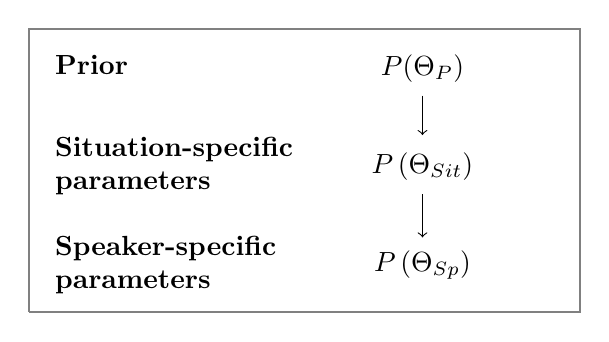
\begin{tikzpicture}
\draw[gray, thick] (0,-0.1) -- (7,-0.1) -- (7,3.5) -- (0,3.5) -- (0,-0.1);
\draw (0, 3.0) node[anchor=west] {\begin{tabular}{l} {\bf Prior} \end{tabular}};
\draw (0, 1.75) node[anchor=west] {\begin{tabular}{l} {\bf Situation-specific} \\ {\bf parameters} \end{tabular}};
\draw (0, 0.5) node[anchor=west] {\begin{tabular}{l} {\bf Speaker-specific} \\ {\bf parameters} \end{tabular}};

\draw (5, 3.0) node {$P(\Theta_P)$};

\draw (5, 1.75) node {$P\left(\Theta_{Sit}\right)$};

\draw (5, 0.5) node {$P\left(\Theta_{Sp}\right)$};


\draw[black,->] (5, 2.65) -- (5, 2.15);


\draw[black ,->] (5, 1.4) -- (5, 0.85);


\end{tikzpicture}
%\includegraphics[width=\columnwidth]{plots/model.pdf}
\caption{Hierarchical model of semantic adaptation. Situation-specific parameters $P(\Theta_{Sit})$ depend on prior beliefs $P(\Theta_P)$ and speaker-specific parameters $P(\Theta_{Sp})$ depend on the situation-specific parameters. \label{fig:model}}
\end{figure}



A second possibility would be to cast the model as a mixture model in which overall production parameters are a 
weighted combination of situation-specific and speaker-specific parameters (and potentially other factors). 
Figure~\ref{fig:mixture-model} shows a sketch of a potential mixture model.
According to such a model, listeners would form both situation-specific and speaker-specific
expectations as a result of adaptation and then combine these expectations to their overall expectations. 
Such a model would also predict the smaller effect size in Experiment~4 since it would predict
that the overall production expectations are influenced by the speaker-specific statistics as 
well as the situation-specific statistics and the latter drive the production expectations to be more similar to
an ``average'' speaker. When listeners are exposed to two identical speakers, on the other hand, the 
situation-specific expectations (which are in line with the speaker type of both exposure speakers) 
would reinforce the speaker-specific expectations and therefore lead to a larger adaptation effect. Future experimental work should adjudicate between the hierarchical and the mixture model account.

\begin{figure}
\center
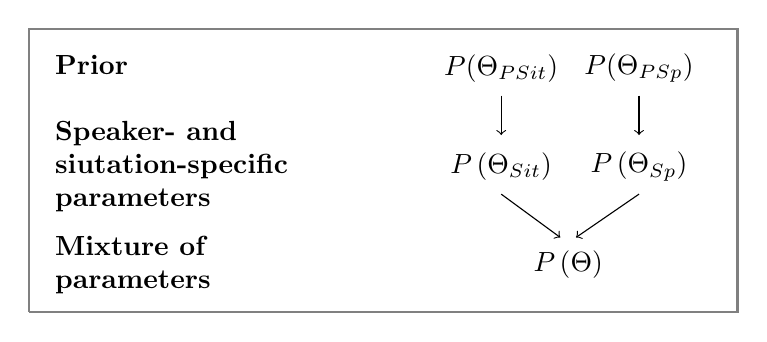
\begin{tikzpicture}
\draw[gray, thick] (0,-0.1) -- (9,-0.1) -- (9,3.5) -- (0,3.5) -- (0,-0.1);
\draw (0, 3.0) node[anchor=west] {\begin{tabular}{l} {\bf Prior} \end{tabular}};
\draw (0, 1.75) node[anchor=west] {\begin{tabular}{l} {\bf  Speaker- and} \\ {\bf siutation-specific} \\ {\bf parameters} \end{tabular}};
\draw (0, 0.5) node[anchor=west] {\begin{tabular}{l} {\bf Mixture of} \\ {\bf parameters} \end{tabular}};

\draw (6, 3.0) node {$P(\Theta_{PSit})$};

\draw (7.75, 3.0) node {$P(\Theta_{PSp})$};


\draw (6, 1.75) node {$P\left(\Theta_{Sit}\right)$};

\draw (7.75, 1.75) node {$P\left(\Theta_{Sp}\right)$};

\draw (6.85, 0.5) node {$P\left(\Theta\right)$};


\draw[black,->] (7.75, 2.65) -- (7.75, 2.15);

\draw[black,->] (6, 2.65) -- (6, 2.15);


\draw[black,->] (7.75, 1.4) -- (6.95, 0.85);
\draw[black,->] (6, 1.4) -- (6.75, 0.85);




\end{tikzpicture}
%\includegraphics[width=\columnwidth]{plots/model.pdf}
\caption{Mixture model of semantic adaptation. Overall production parameters $P\left(\Theta\right)$ are a weighted combination of situation-specific parameters $P\left(\Theta_{Sit}\right)$ and speaker-specific parameters $P\left(\Theta_{Sp}\right)$ . \label{fig:mixture-model}}
\end{figure}

In conclusion, in this chapter, I presented new experimental results from the domain of uncertainty expressions which suggest that speaker-specific semantic adaptation
is a product of forming speaker-specific expectations and forming expectations about the situation independent of the
speaker.
These results raise a number of interesting questions, most pressingly regarding transfer effects to novel speakers, which 
have been observed in other linguistic domains \egcite{Bradlow2008,Xie2018}. In the experiments reported here, the exposure and test speakers
did not differ. This raises the question about whether and to what extent updated expectations transfer to novel speakers whose similarity to the exposure speaker(s) varies.
Both models sketched above lend themselves well to capturing such transfer effects.
In addition, participants saw very similar visual scenes on each trial. Another potential direction would be to study the 
extent of speaker-specific adaptation when listeners encounter more novel scenes during the test phase to investigate to what extent
listeners form speaker-specific expectations independent of other contextual factors.
Answering these
questions will help disentangle the different adaptation processes and give us a better understanding
of how listeners infer meanings in context.



    \chapter{Explaining away}
    
In the previous chapters, I showed that listeners \emph{can} adapt to variable language use. However, the results that I presented so far did not reveal anything about the contextual conditions and limits on adaptation. In principle, it is possible that listeners might update their production expectations regardless of the context of an utterance.  Alternatively, listeners' production expectations, and consequently their adaptive behavior, might be modulated by non-linguistic contextual factors. To illustrate this, consider a speaker $S$ who is in a very good mood and wants to be encouraging. If $S$ tells a listener $L$ ``you'll \textit{probably} win the sweepstake'' when there is only a 60\% chance of winning, $L$ may consider $S$'s use of \textit{probably} instead of a weaker alternative such as \textit{might} to be the result of $S$'s mood. Consequently, $L$ would not necessarily expect $S$ to use \textit{probably} to describe the same event probability when $S$ is in a worse or more discouraging mood.

%To illustrate this, consider a listener who encounters a used car salesman describing obviously mediocre cars with highly positive adjectives such as \textit{amazing}. Being aware of the speaker's incentive to use extremely positive language, the listener will likely not update their beliefs about the speaker's use of evaluative adjectives, and for example, if the same speaker later recommends an ``amazing restaurant'', the listener will likely not conclude that the restaurant is actually mediocre.

The computational model that I presented in Chapter~4 suggests that adaptation may be modulated by contextual factors . According to this model, when interacting with a speaker and observing their language use, listeners integrate their prior beliefs about the speaker's semantic representations and lexical preferences with the observed utterances to arrive at updated speaker-specific production expectations. Given the integration of prior beliefs, this model predicts that the extent to which listeners adapt depends on how they initially expect a speaker to use language. Consequently, contextual factors that affect listeners' expectations about language use should also affect how much listeners adapt to specific speakers. If, given contextual information, a speaker's behavior matches prior expectations, there is no need to adapt.

\begin{figure}
    \centering
    \includegraphics[width=0.75\columnwidth, trim={0 1cm 0 0cm}]{./plots/example-trial.png}
    \caption{Example trial from Experiment 6 and the post-exposure blocks from Experiments 7 and 8.}
    \label{fig:example-trial-ea}
\end{figure}

As I also discussed in Chapter 2, in addition to the model-predicted influence of contextual factors on adaptation, there is empirical evidence from phonetic adaptation: In a phonetic adaptation experiment, \textcite{Kraljic2008} found that without additional information listeners adapted such that their perceptual boundary between /s/ and /sh/ shifted. However, when participants were shown a picture of the speaker with a pencil in their mouth, they explained away the observed signal as a pencil-distorted /sh/-sounding /s/ rather than as an intentionally produced /sh/-sounding /s/. Consequently, they did not adapt, i.e., their perceptual boundary between /s/ and /sh/ did not shift.

In this chapter, I investigate whether listeners explain away otherwise unexpected behavior at the lexical level if they are presented with contextual information that provides a reason for a speaker's productions. Concretely, I investigate whether one contextual factor  -- the speaker's mood -- provides such a reason for otherwise less expected uses of the uncertainty expressions \textit{might} and \textit{probably}  (\textsc{explaining away hypothesis}). However, considering that the studies presented in previous chapters as well as other work on semantic adaptation \cite{Yildirim2016} kept all aspects of the context constant between the exposure and test phase, it could also be that listeners simply learn associations between the use of uncertainty expressions and speakers, independent of other contextual information (\textsc{associative hypothesis}).

I investigate this issue as follows. I first establish that language users have different expectations about a generic speaker's use of uncertainty expressions depending on their beliefs about the speaker's mood (Exp.~6). I then investigate how much participants adapt when they are provided with information about the speaker's mood that makes their use of uncertainty expressions more expected, and compare participants' adaptation behavior to a neutral adaptation setting in which participants do not receive any information about the speaker's mood (Exp.~7). Finally, I investigate the relationship between adaptation and highly unexpected behavior by exposing participants to a speaker whose use of uncertainty expressions is incongruent with their mood (Exp.~8). I find that listeners adapt less when they are presented with a reason for the speaker's behavior. However, surprisingly, I also find that listeners do not adapt more when the behavior is highly unexpected given contextual information, potentially suggesting that there are limits on adaptation.

\section{Experiment 6: Effect of speaker mood}

In Exp.~6, I investigated how one contextual factor, the speaker's mood, affects listeners' expectations about a speaker's use of the uncertainty expressions \textit{might} and \textit{probably} for a range of event probabilities. The choice to manipulate the speaker's mood was guided by the intuition that listeners expect a speaker in a good mood to use uncertainty expressions differently from a speaker in a bad mood. Moreover, mood is a non-inherent property of speakers that can change over time, which is important for Exps.~7 and 8. 

Procedure, materials, analyses, exclusions and predictions were pre-registered on OSF (\url{https://osf.io/5dk7b}).



\subsection{Methods}

\subsubsection{Participants} I recruited 60 participants (20 per condition) from Amazon's Mechanical Turk. 

%We required participants to have a US-based IP address and an approval rating of at least 95\%, as well as to complete a CAPTCHA at the beginning of the experiment. Participants were paid USD 2.20 (approximately USD 12-15/hr).

\subsubsection{Materials and procedure}
%The paradigm is very similar to \cite{Yildirim2016} and \cite{Schuster2019}\jd{shouldn't this only go into the adaptation experiments?}
At the beginning of the experiment, participants were introduced to an airline representative. Depending on the condition, the instructions explained that the representative was having a particularly bad day and feeling pessimistic and angry (\textit{pessimist} condition); that she was having a particular great day and feeling optimistic and helpful (\textit{optimist} condition); or that she was having a normal day (\textit{neutral} condition). In addition to the textual mood information, the drawing of the representative  showed her with an angry face (\textit{pessimist}), a big smile (\textit{optimist}), or a neutral facial expression (\textit{neutral}).

Participants were then instructed that they would see scenes in which a customer of a cheap airline, who had the choice between getting a seat assigned at random or paying \$50 to pick their seat, would ask the representative about their possible seat assignment, to determine the likelihood of getting their preferred seat without paying. As shown in Fig.~\ref{fig:example-trial-ea}, participants could see the seat map and thus determine the number of available window and aisle seats and estimate the probability of getting the preferred seat. On each trial, participants had to indicate how likely they considered the representative to respond with one of the following two  utterances:

\begin{itemize}
    \item You might get a window seat/an aisle seat. (\textsc{might})
    \item You'll probably get a window seat/an aisle seat. (\textsc{probably})
\end{itemize}

Participants indicated their production expectations by distributing 100 points across these two utterances using a slider. If they thought that neither of the two utterances were likely responses, they could assign points to a blanket \textit{something else} option. Participants completed 36 trials: they provided  4 ratings for each of 9 different probabilities of getting a preferred seat, ranging from 0\% to 100\% as indicated by the seat map. Trials were counterbalanced on whether the customer asked for a window or an aisle seat and trial order was randomized.


\subsubsection{Analysis and exclusions}

As in previous experiments, I quantified the production expectations for \textsc{might} and \textsc{probably} by fitting a spline with 4 knots for each participant and expression and computing the area under the curve (AUC) for each of these splines. A larger AUC indicates that an expression was rated highly for a larger range of event probabilities. To compare production expectations across conditions, I computed the difference in AUC between \textsc{might} and \textsc{probably} and compared the average difference across participants in the two conditions.

I excluded participants who provided random responses. Concretely, I excluded participants whose ratings for different event probabilities highly correlated ($r>0.75$) with their average rating, suggesting that they always provided approximately the same rating independent of the event probability. Based on this criterion, I excluded 7 participants (\textit{optimist}: 1, \textit{pessimist}: 3, and \textit{neutral}: 3).

\subsubsection{Predictions}

I predicted that participants expect the \textit{optimistic} speaker to be encouraging and therefore to use \textsc{probably} for a wider range of event probabilities than the \textit{pessimistic} speaker. Conversely, I predicted that participants expect the \textit{pessimistic} speaker to use \textsc{might} for a wider range of probabilities than the \textit{optimistic} speaker. This prediction should be reflected in larger AUC differences in the \textit{pessimist} condition than in the \textit{optimist} condition. Since it was unclear what mood participants attributed to the \textit{neutral} speaker, I only predicted that the mean AUC difference for this third condition should lie between the mean AUC differences of the \textit{optimist} and \textit{pessimist} conditions, with the possibility of being equal to one of the two conditions.

\begin{figure}[t]
    \centering
    \includegraphics[width=0.75\columnwidth, trim={0 0.75cm 0 0cm}]{./plots/norming.pdf}
    \caption{Mean ratings for \textsc{might} and \textsc{probably} for each condition in Exp.~6. Error bars correspond to bootstrapped 95\%-confidence intervals.}
    \label{fig:results-exp6}
\end{figure}

\subsection{Results and discussion}

Fig.~\ref{fig:results-exp6} shows participants' mean ratings for \textsc{might} and \textsc{probably} across the three conditions. As expected, I observe ratings close to 0 for both utterances when there is a 0\% chance of getting the preferred seat (where there is a preference for the \textit{something else} option, not shown), high ratings for \textsc{might} for low event probabilities, and high ratings for \textsc{probably} for high event probabilities. At the same time however, there are also differences across conditions. As the left panel shows, \textsc{might} was rated higher in the \textit{pessimist} condition than in the \textit{optimist} condition for a large range of event probabilities; as the right panel shows, the opposite was true for \textsc{probably}. Ratings in the \textit{neutral} condition were almost identical to the ratings in the \textit{optimist} condition. All these observations were also reflected in the AUC differences: The AUC differences in the \textit{pessimist} condition were greater than in the \textit{optimist} condition ($t(34)=2.51$, $p < 0.05$). The AUC differences in the \textit{neutral} condition -- while numerically slightly larger -- were not significantly different from the differences in the \textit{optimist} condition ($t(34)=0.35$, $p>0.7$).

These results provide evidence that listeners have mood-dependent expectations about a generic speaker's use of uncertainty expressions. In Exp.~7, I investigate whether  speaker mood affects the extent to which listeners adapt to that speaker's use of uncertainty expressions.  %Conditions only differed in the cover story that indicated the speaker's mood, and participants provided different ratings depending on whether they thought the speaker was in a good or bad mood.

%\seb{TODO: relate this to politeness literature.}\jd{not sure this is necessary}

%Given that listeners have different expectations about the production of uncertainty expressions, we expect that information about the speaker's mood also influences the extent to which they adapt to a specific speakers' use of uncertainty expressions. We test this hypothesis in Exp.~2.

\section{Experiment 7: Explaining away}

In an exposure-and-test paradigm, I investigated whether adaptation to a specific speaker is modulated by knowledge about the speaker's mood. As in Chapter~4, I either exposed participants to a speaker who always used \textsc{might} to describe an event probability of 60\% (the ``\textit{cautious}'' speaker) or a speaker who always used \textsc{probably} to describe an event probability of 60\% (the ``\textit{confident}'' speaker). Based on the results of Exp.~6, the behavior of a \textit{cautious} speaker is more expected of a speaker who is having a bad day, and the behavior of a \textit{confident} speaker is more expected of a speaker who is having a good day. I thus hypothesized that participants' beliefs about the speaker's mood influence how much they adapt: If the speaker's behavior is mood-congruent, I expected participants to experience a weaker expectation violation and adapt less than in the neutral conditions.

Procedure, materials, analyses, exclusions and predictions were pre-registered on OSF (\url{https://osf.io/4zpt6}).

\subsection{Methods}

\subsubsection{Participants} I recruited 320 participants (80 per condition) from Amazon's Mechanical Turk. 

\begin{table}
\centering
\begin{tabular}{r|c c|c c }
\toprule 
     \textbf{Condition} & \textit{\textbf{pessimist}} & \textit{\textbf{cautious}} & \textit{\textbf{confident}} & \textit{\textbf{optimist}} \\
     \textbf{Mood} & bad & neutral & neutral & good  \\ \midrule
     $p=25\%$ & \multicolumn{2}{c |}{--} & \multicolumn{2}{c }{\textsc{might} x5} \\
     \cellcolor{LightGray} $p=60\%$ & \multicolumn{2}{c |}{\cellcolor{LightGray} \textsc{might} x5} & \multicolumn{2}{c }{\cellcolor{LightGray} \textsc{probably} x5}\\
     $p=90\%$ & \multicolumn{2}{c |}{\textsc{probably} x5} &  \multicolumn{2}{c }{--} \\
     $p=100\%$ & \multicolumn{2}{c |}{\textsc{bare} x3} & \multicolumn{2}{c }{\textsc{bare} x3} \\
     \bottomrule
\end{tabular}
\caption{Overview of exposure utterances in Exp.~7. $p$ indicates the proportion of preferred available seats shown on the seat map while the speaker produced the utterance. Critical trials are highlighted in gray. \label{tbl:exposure-overview-exp7}}
\end{table}


\subsubsection{Materials and procedure}

The first block of the experiment consisted of an exposure phase with 13 trials (5 critical, 8 filler). On each trial, participants first saw a scene in which a customer asked about a specific seat and a seat map which indicated the number of available window and aisle seats (see top part of Fig.~\ref{fig:example-trial-ea}). To make sure participants paid attention to the seat map, they were then asked to rate how likely the customer  was to get the preferred seat. They then listened to a pre-recorded response from the airline representative. Exposure trials were identical across the \textit{pessimist} and \textit{cautious speaker} conditions and identical across the \textit{optimist} and \textit{confident speaker} conditions but differed across these two pairs of conditions (see Table~\ref{tbl:exposure-overview-exp7} for an overview): In the \textit{pessimist} and \textit{cautious speaker} condition, there were 5 critical trials in which the representative described a 60\% probability of getting the preferred seat with ``You might get one'' (\textsc{might}); in the \textit{optimist} and \textit{confident speaker} conditions, the speaker responded with ``You'll probably get one'' (\textsc{probably}). 5 filler trials in the \textit{pessimist}/\textit{cautious speaker} conditions consisted of \textit{probably} responses   when there was a 90\% preferred seat probability, and 5 filler trials in the \textit{optimist}/\textit{confident speaker} conditions combined \textit{might} with a 25\% preferred seat  probability. Finally, 3 additional filler trials in all four conditions consisted of the response ``You'll get one'' (\textsc{bare}) when it was 100\% likely for the customer to get their preferred seat. Filler trials were intended to boost credibility of the speaker.

The exposure block was followed by another instruction, informing participants in all conditions that it was a week later and that the airline representative was having a normal day, followed by another manipulation check asking participants to rate how they thought the representative was feeling. 

The last block of the experiment was identical to the trials in Exp.~6: participants completed 36 trials and rated how likely they thought it was that the speaker produced \textsc{might}, \textsc{probably} or \textit{something else} for 9 different preferred seat probabilities.

\subsubsection{Analysis and exclusions}

I computed the AUC difference between the splines for  \textsc{might} and \textsc{probably} for each participant as in Exp.~6. I again excluded data from participants providing random responses, which led to 52 exclusions (\textit{pessimist}: 9, \textit{cautious}: 14, \textit{optimist}: 18, \textit{confident}: 11).

\begin{figure}[t]
    \centering
    \includegraphics[width=0.75\columnwidth, trim={0 0.75cm 0 0cm}]{./plots/explaining-away.pdf}
    \caption{Mean ratings for \textsc{might} and \textsc{probably} for each condition in Exp.~7. Error bars correspond to bootstrapped 95\%-confidence intervals.}
    \label{fig:results-exp7}
\end{figure}
\subsubsection{Predictions}

I expected that participants would adapt to the use of uncertainty expressions by the different speakers and update their expectations. Further, in line with the \textsc{explaining away hypothesis}, participants in the \textit{pessimist} and \textit{optimist} conditions, who should experience less of an expectation violation, should adapt less than participants in the other two conditions. In terms of the AUC difference (AUC(might) - AUC(probably), I therefore expected the following ordering: \textit{cautious speaker} $<$  \textit{pessimist} $\leq$ \textit{optimist} $<$ \textit{confident speaker}.

However, in Exp.~6, I also found that the ratings in the \textit{neutral} condition did not significantly differ from the ratings in the \textit{optimist} condition. This suggests that listeners' initial expectations about the speaker's mood and the associated production expectations only slightly differ across the \textit{optimist} and the \textit{confident speaker} conditions and therefore I also expected similar adaptation behavior in these two conditions.\footnote{This intuition was further confirmed in a pilot study with 10 participants per condition, which I conducted prior to pre-registration. In the pilot, I found the expected ordering for the \textit{cautious speaker}, \textit{pessimist}, and \textit{confident speaker} conditions but the difference between the \textit{optimist} and \textit{confident speaker} condition was so small that I would have needed more than 205 participants per condition to achieve power of $\beta=0.8$.} I therefore, while expecting the numerical ordering described above, expected and pre-registered only significant differences between the \textit{pessimist} and \textit{cautious speaker} conditions, and between the \textit{cautious speaker} and \textit{confident speaker} conditions.

If listeners' adaptation behavior is not affected by contextual information, in accordance with the \textsc{associative hypothesis}, there should be no difference between the \textit{cautious speaker} and  \textit{pessimist} conditions and no difference between the \textit{confident speaker} and \textit{optimist} conditions.

\subsection{Results and discussion}

Fig.~\ref{fig:results-exp7} shows the mean ratings for \textsc{might} and \textsc{probably} for the four conditions. The results are consistent with the predictions according to the \textsc{explaining away hypothesis}: First, participants in the \textit{confident speaker} condition rated \textsc{probably} higher for a larger range of event probabilities than in the \textit{cautious speaker} condition and the opposite was true for \textsc{might}. This pattern is also reflected in the mean AUC difference, which is larger in the \textit{cautious speaker} condition than in the \textit{confident speaker} condition ($t(133)=5.18$, $p < 0.001$). This result replicates the adaptation effect that I found in previous experiments and suggests that this seat map paradigm is also suited for studying adaptation in the use of uncertainty expressions.

Second, I also observe differences between the \textit{cautious speaker} and \textit{pessimist} conditions. The mean AUC difference is larger in the \textit{cautious speaker} condition than in the \textit{pessimist} condition  ($t(135)=2.38$, $p < 0.02$).

Third, I also observe a numeric difference between the \textit{confident speaker} and \textit{optimist} conditions. Numerically, the AUC difference is larger in the \textit{optimist} condition than in the \textit{confident speaker} condition, but not significantly so ($t(129) =1.61$, $p = 0.11$).

Lastly, as shown in Fig.~\ref{fig:manip-check-exp7}, participants in the \textit{optimist} and \textit{pessimist} condition updated their beliefs about the mood after I instructed them that the speaker was now in a normal mood, suggesting that this instruction was sufficient to update participants' beliefs about the speaker's mood. As expected, participants in the two neutral conditions did not change their beliefs about the speaker's mood. 

\begin{figure}[t]
    \centering
    \includegraphics[width=.6\columnwidth, trim={0 0.75cm 0 0cm}]{./plots/mood-differences-exp2.pdf}
    \caption{Differences in mood ratings in Exp.~7. The x-axis indicates the difference between the mood rating before the exposure block and the mood rating before the test block.}
    \label{fig:manip-check-exp7}
\end{figure}


The results from this experiment provide evidence for listeners explaining away otherwise unexpected productions if they are presented with a reason for the speaker's behavior, and are predicted by the \textsc{explaining away} account. 

However, with additional stipulations, these results are also compatible with the \textsc{associative} account. One aspect of the context, the speaker's mood, changed between the exposure block and the test block in the \textit{pessimist} and \textit{optimist} conditions but not in the other two conditions. Therefore, it could be that this difference between the blocks leads to weaker associations between utterances and the context and therefore I observe less adaptation in the \textit{pessimist} and \textit{optimist} conditions. To evaluate this possibility, I conducted Exp.~8.


\section{Experiment 8: Incongruent conditions}

In Exp.~8, I investigated participants' adaptation behavior when the speaker's use of uncertainty expressions was incongruent with the information about the speaker's mood, i.e., a speaker in a bad mood using uncertainty expressions like the \textit{confident speaker} in Exp.~7, or a speaker in a good mood behaving like the \textit{cautious speaker}. According to the \textsc{explaining away} account, this should lead listeners to experience a stronger expectation violation than in the neutral and congruent conditions in the previous experiment and therefore listeners should adapt more.  According to the \textsc{associative} account, on the other hand, listeners should adapt less than in the neutral conditions because according to this account, the smaller adaptation effect that I found in the \textit{optimist} and \textit{pessimist} conditions in the previous experiment was caused by a difference between the exposure phase and the test phase, which is still present in this experiment.


\subsection{Methods}

\subsubsection{Participants} I recruited 160 participants (80 per condition) from Amazon's Mechanical Turk.

\subsubsection{Materials and procedure}

\begin{table}
\centering
\begin{tabular}{r|c | c }
\toprule 
     \textbf{Condition} & \textit{\textbf{pessimist incongr.}} & \textit{\textbf{optimist incongr.}} \\
     \textbf{Mood} & bad  & good  \\ \midrule
     $p=25\%$ & \textsc{might} x5 & -- \\
     \cellcolor{LightGray} $p=60\%$ &  \cellcolor{LightGray} \textsc{probably} x5 & \cellcolor{LightGray} \textsc{might} x5 \\
     $p=90\%$ & -- &  \textsc{probably}  \\
     $p=100\%$ & {\textsc{bare} x3} & {\textsc{bare} x3} \\
     \bottomrule
\end{tabular}
\caption{Overview of exposure utterances in Exp.~8. $p$ indicates the proportion of preferred available seats shown on the seat map while the speaker produced the utterance. Critical trials highlighted in gray.\label{tbl:exposure-overview-exp8}}
\end{table}


The procedure was identical as in Exp.~7. There were two conditions: \textit{optimist incongruent} and \textit{pessimist incongruent}. The \textit{optimist incongruent} condition showed a speaker in a good mood who produced the same utterances as the \textit{pessimist} and \textit{cautious} speaker from the previous experiment. The \textit{pessimist incongruent} condition showed a speaker in a bad mood who produced the same utterances as the \textit{optimist} and \textit{confident} speakers in Exp.~7. See Table~\ref{tbl:exposure-overview-exp8} for an overview of the exposure trials.

\subsubsection{Analysis and exclusions}

Analyses and exclusions were identical to the ones of Exp.~7. I excluded 27 participants (\textit{optimist incongruent}: 15, \textit{pessimist incongruent}: 12).

\subsubsection{Predictions}

I predicted that participants would adapt to different uses of uncertainty expressions: I expected the AUC difference in the \textit{optimist incongruent} condition to be larger than in the \textit{pessimist incongruent} condition. I further predicted that listeners experience a stronger expectation violation than in the neutral conditions in Exp.~7. I therefore also predicted the AUC difference in the \textit{optimist incongruent} condition to be larger than in the \textit{cautious speaker} condition, and the AUC difference in the \textit{pessimist incongruent} condition to be smaller than in the \textit{confident speaker} condition.

\subsection{Results and discussion}

Fig.~\ref{fig:results-exp8} shows the mean ratings for \textsc{might} and \textsc{probably} for the two conditions in this experiment as well as the mean ratings from the neutral conditions from Exp.~7. As this plot shows, participants adapted to the different uses of uncertainty expressions. The mean AUC difference in the \textit{optimist incongruent} condition was larger than in the \textit{pessimist incongruent} condition ($t(131)=5.90$, $p<0.001$). However, unexpectedly, participants did not adapt more in the incongruent conditions than in the neutral conditions. The mean AUC difference in the \textit{optimist incongruent} condition was not larger than in \textit{cautious} condition ($t(129)=0.004$, $p=0.99$), and the mean AUC difference in the \textit{pessimist incongruent} condition was not significantly smaller than in the \textit{confident} condition ($t(135)=-1.18$, $p=0.24$).

\begin{figure}[t]
    \centering
    \includegraphics[width=.75\columnwidth, trim={0 0.75cm 0 0cm}]{./plots/incongruent.pdf}
    \caption{Mean ratings for \textsc{might} and \textsc{probably} for the two conditions in Exp.~8 as well as the neutral conditions in Exp.~7. Error bars correspond to bootstrapped 95\%-confidence intervals.}
    \label{fig:results-exp8}
\end{figure}

In this experiment, I again replicated the adaptation effect. However, I did not find a significantly stronger adaptation effect across the two incongruent conditions in this experiment as compared to the neutral conditions from the previous experiment, despite the fact that listeners should have experienced a stronger expectation violation.

What do these results imply for the \textsc{explaining away} and \textsc{associative} accounts that I presented above? Together with the results from Exp.~7, the results from this experiment are unexpected under the \textsc{associative} account: if the reason for participants adapting less in the \textit{pessimist} condition had been the difference in context between the exposure and test blocks, I would have expected less adaptation in this experiment as well.

However, I also did not find stronger adaptation, as I would have expected under the \textsc{explaining away} account. I can only speculate about the reasons for this, but two explanations seem likely. First, given that there was a numerical difference between the \textit{pessimist incongruent} and \textit{confident} conditions in the expected direction, it could be that my experiment was underpowered to detect a potentially very small effect. However, a power analysis suggests I would need more than 500 participants per condition to achieve power of $\beta=0.8$ and therefore I did not explore this option further.

Second, it could be that there is a limit on how much listeners can adapt and that this limit is already reached in the neutral conditions. If this was the case, listeners could still experience a stronger expectation violation when the behavior is incongruent with contextual factors but this stronger violation still does not lead to stronger adaptation. 

%Third, given that the combination of utterances was incongruent with the speaker's mood, and therefore potentially unexpected of a reliable speaker, it could also be that participants were drawing a higher-level inference that the speaker was unreliable \cite<e.g.,>{Grodner2011}.\jd{though this could affect responses in various ways -- is it worth saying this? otherwise perhaps we leave it out after all?}

\section{General Discussion}

In this chapter, I showed in three experiments that language users have different expectations about the use of uncertainty expressions depending on their beliefs about the speaker's mood, and that this difference in expectations affects the extent of semantic adaptation. The results suggest listeners explain away otherwise unexpected behavior when they are presented with a cause, similarly as \textcite{Kraljic2008} found for phonetic adaptation.

The results presented here further largely confirm a prediction made by computational models of adaptation, namely that the extent of adaptation depends on how much observed behavior deviates from prior expectations. Similar results have been found for syntactic priming \cite{Jaeger2013} and are predicted by connectionist models of syntactic learning \cite{Chang2006} as well as Bayesian probabilistic models of syntactic adaptation \cite{Kleinschmidt2012}.

However, the results from Exp.~8 suggest that expectation violation is not the only factor that influences adaptation and that there potentially exist limits to how much listeners can adapt, an issue that I will discuss further in the next chapter. 

    
    \chapter{Conclusions}
    %\subsection{Methodological implications}

%My results also have implications for conducting psycholinguistic experiments. First,
%the finding that listeners adapt to the statistics of their environment within a short experiment
%suggests that experimenters should be cognizant of potential adaptation effects when probing
%production expectations or interpretations of uncertainty expressions \parencite[see also][]{Jaeger2010}. 

%Further, the results of Experiment~1, and in particular, the finding
%that participants' expectations about the use of utterances in the experiment strongly depended on
%the alternative utterances that we provided, highlights the need to be cautious about drawing general conclusions about expectations of use from single experiments. For example,
%had we only considered the results from the \textit{bare-might} condition (see \figref{fig:norming-results-main}),
%we might have concluded that ``might'' is an expected expression to communicate an event probability of 75\%,
%whereas if we had only considered the results from the \textit{might-probably} condition we might have instead concluded that it is \emph{not} an expected expression to communicate an event probability of 75\%.
%This is where explicit modeling of the sort we have engaged in here is hugely helpful: formulating a concrete linking function which models the effects of 
%alternatives allows for inferring the latent meanings of utterances by combining data from different experiments \parencite[see also][for similar approaches]{Franke2014,Peloquin2016}.

% \subsection{Limitations}

%One limitation of the present research is that the experimental paradigm is not interactive and that participants likely 
%engaged in meta-linguistic reasoning in providing production expectation and interpretation ratings. 
%While we tried to make the communicative situation depicted in the experiments natural,
%the paradigm is clearly different from everyday dialog. This limitation was necessary for the tight coupling between the experimental work
%and the model simulations that allowed us to investigate what kind of representations listeners update during adaption; in a more
%naturalistic and unconstrained setting, we would not have been able to obtain information about listener's production expectations and about their
%uncertainty in both production expectations and interpretations. However, considering that our task was different from everyday interactions, investigating
%to what extent the results in the present research translate to less scripted and more interactive settings is an important area for future research. Employing measures like eye movements or mouse-tracking could provide insight into whether participants' updated beliefs affect online language processing, i.e.~where meta-linguistic reasoning is unlikely to occur. In this vein, mouse-tracking has recently been
%employed  to investigate the incremental nature of adaptation in the domain of  prosodic cues \cite{Roettger2019}. Both eye-tracking and mouse-tracking experiments 
%allow for implementing more natural interpretation tasks while still providing information about participants' uncertain beliefs via fixation patterns or cursor trajectories.

%\epigraph{Da steh ich nun, ich armer Tor, \\
%und bin so klug als wie zuvor.} {\textit{Faust}\\ \textit{Johann Wolfgang von Goethe}}

At the beginning of this dissertation I raised the question of how listeners deal with production variability at the semantic-pragmatic level. The experiments that I presented in the previous chapters provided answers to several important subquestions of this larger issue: In Experiment~2, I showed that after brief exposure to a speaker, listeners rapidly update their expectations about that speaker's use of uncertainty expressions to closer match the speaker's behavior. In Experiment~3, I showed that this update in production expectations directly transfers to interpretations and consequently, listeners form speaker-specific interpretations of uncertainty expressions. In Experiments~4 and 5, I showed that listeners can adapt to multiple speakers and that they also adapt to contextual factors independent of the speaker such as the situation in which an utterance is produced. Finally, in Experiments~7 and 8, I showed that the extent of adaptation depends on prior expectations of language use and that to some extent listeners explain away otherwise unexpected behavior when presented with a cause.

Moreover, the modeling results in Chapter~4 provided novel insights into the cognitive processes responsible for adaptation. I found that a model based on Bayesian belief updating predicts both production expectation and comprehension data well. Further, I found that a model that assumes that listeners update both semantic representations and speaker preferences predicts post-adaptation behavior better than models that assume that only one of these two types of representations are updated.

What do these results tell us about the human comprehension system? As I mentioned in the introduction, there have been three proposals for dynamic comprehension systems that can deal with variability: \textit{normalization} of input, \textit{alignment} of linguistic representations, and \textit{adaptation} to variable language use. As I also discussed in Chapter~4, \textit{normalization} is not applicable in the interpretation of uncertainty expressions since listeners are faced with the challenge of mapping a discrete expression to a continuous event probability rather than mapping a continuous property to a discrete symbol as is the case with the recognition of phonemes. The other two accounts, \textit{alignment} and \textit{adaptation}, on the other hand, were both plausible candidates for the processes leading to partner-specific in the interpretation of uncertainty expressions.

The experimental evidence that I provided in this dissertation adjudicates between these two accounts. On the one hand, all my results are compatible with a sophisticated adaptation account according to which listeners constantly update speaker expectations based on statistical input. This account predicts that listeners form speaker-specific production expectations, that listeners form speaker-specific interpretations, that listeners can adapt to multiple speakers, and that listeners' adaptation behavior depends on prior production expectations, which may be affected by non-linguistic contextual factors.

An alignment account, on the other hand, is only compatible with some of the findings from the experiments above. If one assumes that linguistic representations are linked to contextual representations,  an alignment account predicts that listeners align their linguistic representations (and thus also their speaker expectations and interpretations) to a single speaker. However, importantly, this account fails to account for adaptation to multiple speakers. As I explained in Chapter~2, this account is based on the assumption that partner-specific behavior is a result of residual activation of linguistic representations from comprehending and producing previous utterances in interaction. Since residual activation  of representations decreases over time, one would expect partner-specific behavior to be limited to interactions with the most recent interlocutor rather than -- as I found in Experiment~4 -- listeners forming different production expectations for multiple speakers. Further, an alignment account, which assumes that partner-specific behavior is an by-product of automatic activation of linguistic representations, does not predict the modulation of adaptation by non-linguistic contextual factors that I demonstrated in Chapter~6. 

\section{Generalizability of findings}

My investigations all focused on one class of linguistic expressions, namely uncertainty expressions. This raises the question
to what extent one expects the findings presented here to generalize to other linguistic phenomena.

Throughout this dissertation, I made the assumption that uncertainty expressions have a threshold semantics. Similar semantic
representations have also been successful in predicting the use of quantifiers \egcite{Scholler2017} and gradable adjectives \egcite{Kennedy2007}. Given
the parallels in meaning representations, I expect my findings to directly transfer to these two classes of linguistic expressions, and in fact, 
the results by \textcite{Yildirim2016} provide direct evidence that listeners adapt to variable use of quantifiers, and recent work by \textcite{Xiang2020} 
provides evidence that listeners also adapt to variable use of gradable adjectives.

More abstractly, the threshold distributions can be seen as a property of the lexicon and updating beliefs about threshold distributions can be seen as
updating beliefs about the lexicon. Under this view, it seems likely that many of the results in this dissertation apply more generally to the interpretation of most or all linguistic expressions.
In interaction, listeners can update their beliefs about the speaker's lexicon and learn more precise mappings between expressions and meanings. Evidence for such behavior comes from  experiments and models simulating the formation of conceptual pacts \cite{Hawkins2017}. According to their model, interlocutors update their beliefs about the mapping of referring expressions
to referents in a repeated reference game of describing abstract tangram figures.

Importantly, however, I do not want to imply that listeners will readily update their production expectations and interpretations for any type of expressions. For example, a listener will likely not
update their beliefs about a speaker's mapping for the word \textit{dog} in response to observing the speaker use \textit{dog} to refer to cats.\footnote{They may, however, draw other inferences such as that the speaker does not know what a dog is or that the speaker is uncooperative.} To see why this is the case, recall that one important component of the adaptation model that I presented above are prior beliefs about a speaker's productions before interacting with the speaker. I expect listeners' prior beliefs about the mapping of \textit{dog} to exhibit very little variance, since language users generally seem to agree what kind of objects \textit{dog} refers to. Therefore any lexicon in which \textit{dog} refers to cats, will have extremely low prior probabilities and thus the model predicts that evidence of a speaker using \textit{dog} to refer to cats will have very limited effects on posterior beliefs. In cases in which there is inter-speaker variability as with uncertainty expressions or abstract tangram figures, on the other hand,  listeners' prior beliefs exhibit more uncertainty and therefore observed behavior has a stronger effect on posterior beliefs and ultimately post-adaptation behavior.

Finally, it is also noteworthy that my results highlight a lot of parallels between phonetic adaptation behavior and semantic-pragmatic adaptation behavior. For example, I found that more exposure leads to stronger adaptation, as in phonetic adaptation \parencite{Vroomen2007}; I found that,  if listeners are presented with a cause,  they explain away otherwise unexpected behavior, as in phonetic adaptation \parencite{Kraljic2008}, and similarly as for phonetic adaptation \parencite{Kleinschmidt2015}, a model based on Bayesian belief-updating predicts post-adaptation behavior. While there is no evidence for this beyond these parallels, this might suggest that listeners employ similar processes in learning speaker-specific behaviors at all linguistic levels.



\section{Limitations}

One limitation of the present research is that the experimental paradigm is not interactive and that participants may have 
engaged in meta-linguistic reasoning in providing production expectation and interpretation ratings. 
While I tried to make the communicative situation depicted in the experiments natural,
the paradigm is clearly different from everyday dialog. This limitation was necessary for the tight coupling between the experimental work
and the model simulations that allowed me to investigate what kind of representations listeners update during adaption; in a more
naturalistic and unconstrained setting, I would not have been able to obtain information about listener's production expectations and about their
uncertainty in both production expectations and interpretations. 

Further, I did not systematically investigate to what extent listeners draw higher-level inferences rather than adapting to individual expressions. For example, it 
could be that listeners infer that the speaker wants to be very encouraging when interacting with the child rather than learning something about the speaker's mapping of
uncertainty expressions to event probabilities. While it seems likely that higher-level inferences also affect interpretations, I consider it unlikely that higher-level inferences are the
sole cause for the observed behavior in my experiments. In Chapter~3, I presented results that show that the expressed preference of the child had only a very small effect on
production expectations. Further, in the control conditions in  the explaining away experiment in Chapter~6, I was able to replicate the effects without a child being the fictional
 interlocutor of the experimental speaker. Thus, while it will be important to investigate the exact contributions of higher-level inferences, the aggregate results in 
 this dissertation do not provide evidence for a strong effect of higher-level inferences on post-adaptation behavior.

Similarly, in the model comparisons in Chapter~4, I only considered two types of beliefs that may change as a result of adaptation: beliefs about the semantics
and about preferences. While the model comparisons provided strong evidence that listeners update beliefs about the semantics, the evidence for listeners also updating
preferences was weaker and a model that allowed both types of beliefs to be updated only marginally improved the model's predictive power. 
Further, it could be that these additional parameters in the model that allows updates to preferences are in fact capturing the variance of other factors such as social factors. 
Thus, more model comparisons that consider additional factors should be conducted. However, the experimental results in this dissertation and by \textcite{Yildirim2016}
also provide independent evidence for listeners tracking speaker preferences. \textcite{Yildirim2016} and I found that varying the ratio of productions with different uncertainty expressions also has a small effect on post-adaptation behavior: 
for example, if listeners are exposed to an equal number of productions with \textit{might} and \textit{probably}, their post-adaptation production expectations exhibit less of a bias towards either
of these expressions than when they are exposed to a speaker who uses one of these expressions more often than the other.  This suggests that listeners infer preferences for uncertainty expressions depending on the frequency with which a speaker uses different terms.

Moreover, while I argued that there are a lot of similarities between phonetic adaptation and semantic-pragmatic adaptation, I also have not shown directly
that these processes use shared cognitive mechanisms and it could be that despite the similarity in behavioral results phonetic and semantic-pragmatic
are two distinct phenomena at the implementational level. This also raises the question whether \textit{adaptation} is indeed the correct term
for the phenomenon that I have been discussing. Considering that I have argued that semantic-pragmatic adaptation involves learning about a speaker's
lexicon, the process may be considered more similar to word learning and would therefore potentially be described by a term such as \textit{continuous word learning}. 

Lastly, I portrayed adaptation as a long-term phenomenon that cumulatively improves communication with known interlocutors.
However, in all my experiments, the test phase immediately followed the exposure phase and it remains an open question
whether adaptation to individual speakers indeed persists over longer periods of time (as has been established for phonetic and syntactic
adaptation; e.g., \citeauthor{Xie2018}, \citeyear{Xie2018}; \citeauthor{Kroczek2017}, \citeyear{Kroczek2017}).

\section{Future directions}

One advantage of computational models such as the one that I presented in this dissertation is that they make precise quantitative predictions which can
be subsequently tested in experiments. In this final section, I will discuss several predictions that the model makes and sketch how they could be investigated experimentally.

First, the model predicts that adaptation is incremental and listeners should incrementally update their beliefs following each interaction. While my experiments showed that more exposure leads to more adaptation, I have not systematically investigated the predicted incremental nature of semantic-pragmatic adaptation. One important future direction is therefore to employ paradigms in which exposure and test trials can be combined such as a visual world eye-tracking or mouse-tracking paradigm.  In this vein, mouse-tracking has recently been
employed  to investigate the incremental nature of adaptation in the domain of  prosodic cues \cite{Roettger2019}, and a similar paradigm could be used to study semantic-pragmatic adaptation. Another advantage of using an online measure would be that eye-tracking and mouse-tracking experiments allow for 
implementing more natural interpretation tasks while still providing information about participants' uncertain beliefs via fixation patterns or cursor trajectories,
and these experiments could also provide insight into whether participants' updated beliefs affect online language processing, i.e., where meta-linguistic reasoning is unlikely to occur.

Second, as I mentioned repeatedly, the model predicts that adaptation should depend on the extent of uncertainty reflected in prior beliefs. If listeners don't exhibit uncertainty about a speaker's productions, no or very little adaptation should occur. If, however, listeners exhibit a lot of uncertainty about a speaker's productions, then the model predicts
very rapid adaptation. This relationship between uncertainty in prior beliefs and adaptation behavior holds for the uncertainty expressions that I investigated: I found in Experiment~1 that listeners exhibit uncertainty about a generic speaker's productions. However, whether this relationship holds more generally, and whether listeners adapt much less if there is less prior uncertainty remains an open question. 

Studying this relationship between prior uncertainty and adaptation could likely be done in a comparative study with different classes of expressions. For example, if listeners exhibit different levels of prior uncertainty regarding a generic speaker's use of uncertainty expression, quantifiers, and gradable adjectives, one could run exposure-test experiments for expressions from all of these classes. The model would predict that all things being equal the size of the adaptation effect should correlate with prior uncertainty.

Another important question concerns generalization from one speaker to another speaker, or from one situation to another situation. In all the experiments reported in this dissertation the speaker's identity and all other contextual factors were the same across the exposure and test phase. One important future direction is thus to also study adaptation effects when one or more aspects of the context change. 

Results from generalization experiments could also help adjudicate between the mixture model and the hierarchical model that I discussed in Chapter~5. If the situations between the exposure and test phase are considerably different (which may be challenging to achieve given that being in an experiment may be an important contextual factor), the hierarchical model predicts that we should not see speaker-specific adaptation. This behavior is predicted by the hierarchical model  because according to this model, speaker-specific parameters are tied to a situation and if the situation changes, the model predicts that speaker expectations are guided by an independent set of speaker-specific parameters that are only linked to the novel situation. The mixture model, on the other hand, would predict transfer of speaker-specific behavior from one situation to another.

Finally, in Chapter~6, I speculated that there may be limits to adaptation and that these limits are the reason for the lack of a larger adaptation effect as compared to a control condition when the observed speaker behavior was highly incongruent with the expected behavior. However, given the limited data on this issue, the conclusions on this issue remain highly speculative and a future study should investigate whether we also observe limitations on adaptive behavior in other scenarios. For example, it could be that we would observe similar limitations in the absence of non-linguistic contextual factors if we made the exposure speaker's behavior more extreme. If this is the case, it could be that individual belief updates are capped and at some point higher surprisal no longer leads to larger belief updates in order to prevent too extreme deviations from what is expected. Thus, if limited adaptation behavior can be observed in multiple scenarios, another important future direction would be to study the relationship between prior surprisal and the size of the adaptation effect.

\pagebreak

To conclude, the work reported in this dissertation provided multiple new insights into how listeners deal with variability at the semantic-pragmatic level. The reported investigations have highlighted the dynamicity of the language comprehension system and the novel computational model will hopefully serve as a starting point for many additional investigations into how listeners interpret utterances in variable environments.




   \appendix
    
\chapter{Effect of color in Experiment~1}



As mentioned in a footnote, I ran the norming studies in three batches using three slightly different procedures across conditions. I originally ran condition 0 (\emph{bare-might}) as a pilot condition. In the results, I noted that participants did not differ in their ratings depending on whether the girl asked for a blue or an orange gumball ($R^2(27)=0.997$ between mean ratings for blue and orange trials). To lower the number of trials, I therefore asked each participant to provide ratings for only one of the two colors (randomized across participants) for the next batch of conditions (conditions 1-14). I found that in some conditions, this led to small differences in ratings between participants who always rated utterances with \emph{blue} and participants who always rated utterances with \textit{orange} ($R^2(27)$ between $0.864$ and $0.984$). I hypothesize that this is a result of participants paying less attention if they were asked to do exactly the same task over and over again (in condition 0, the color and the associated utterances could change across trials). In order to verify the stability of our results, I replicated one of the conditions, condition 5 (\emph{might-probably}), and asked participants to provide two ratings for each color and gumball proportion. I found that despite the lower correlation between average ratings for utterances with \emph{blue} and utterances with \emph{orange} in the original run ($R^2(27)=0.929$), there was a very high correlation between the average ratings independent of the color of the original study and the average ratings of the replication ($R^2(27)=0.975$), which suggests that the average ratings largely do not depend on whether I ask participants to provide ratings for both colors or just one color. Nevertheless, I used the modified procedure in which I asked participants to provide 2 ratings for each color and gumball proportion for the last batch of conditions (conditions 15-20). In all conditions in which I asked participants to provide ratings for utterances with both colors, the correlation between average ratings for utterances with \emph{blue} and utterances with \emph{orange} was almost perfect ($R^2(27)>0.988$).



\chapter{Additional results of Experiment~1.}


Figures~\ref{fig:norming-results-1} and \ref{fig:norming-results-2} show the results from all conditions in Experiment~1. 

\begin{figure}[h!]
\includegraphics[width=\textwidth]{plots/fig-B1-pre\string_test\string_s1.pdf}
\caption{Results of Experiment~1 -- Part 1. Error bars correspond to bootstrapped 95\%-confidence intervals. \label{fig:norming-results-1}}
\end{figure}

\begin{figure}[h!]
\includegraphics[width=\textwidth]{plots/fig-B2-pre\string_test\string_s2.pdf}
\caption{Results of Experiment~1  -- Part 2. Error bars correspond to bootstrapped 95\%-confidence intervals. \label{fig:norming-results-2}}
\vspace{4cm}

\end{figure}


\chapter{Model implementation details}

The model presented above poses some challenges for performing Bayesian data analysis with considerable amounts of data. 
Concretely, the integral over threshold distributions in the expected pragmatic speaker model $ES_1$ (repeated here) makes it hard to compute 
the distribution $ES_1$ given a set of parameters $\Theta$.

$$ES_1\left(u_e \mid \phi \right) = \int P(c) \int_0^1 P(\theta) S_1\left(u _e\mid \phi, \theta, c\right) d\theta \  d c$$

The reason for this is two-fold: First, there is no analytical solution for this integral, and second, since $S_1$ depends on
thresholds for all uncertainty expressions $P(\Theta)$ is a multidimensional distribution which cannot be easily approximated.

I solve this issue by introducing two approximations. First, I discretize the threshold distributions by distributing the probability mass
of the Beta distributions across 20 equally-wide bins, resulting in a discrete probability distribution $P_{d}(\theta)$ (see \cite{Tessler2019} for a similar approach). Since all event probabilities for which participants were asked to provide ratings in the
experiments were multiples of 5\%, we do not lose any accuracy and gain the advantage that we can now sum over a discrete probability space:\footnote{In my data analysis procedure, I assumed that the 
distribution over cost functions, $P(c)$, is a delta distribution which assigns all probability mass to the condition-specific cost function 
$c(u, \mathscr{C})$ parameterized by the cost parameter $\gamma$. Since this implies that $P(c)$ is zero for all other cost functions, we can omit the integral and replace $c$ 
with the condition-specific cost function, which I implicitly did here.}
$$ES_1\left(u_e \mid \phi \right) = \sum_{\theta} P_{d}(\theta) S_1\left(u _e\mid \phi, \theta, c\right)$$

While this approximation can in theory be computed exactly, its computation remains intractable even 
for the small number of utterances that I included in the model presented above. Note that the discrete version of the
vector of thresholds $\theta$ has one dimension with 20 possible values for each utterance, which implies
there are $20^{|U|}$ possible assignments of $\theta$. This means for estimating parameters for 
a model with 7 utterances, I would have to sum over $20^{7}=1.28 \times 10^9$ 
parameterizations of the pragmatic speaker model $S_1$ to compute the likelihood for one 
sample of parameters in the BDA. 

I solve this problem through another approximation, which exploits the fact that 
$S_1(u _e \mid \phi, \theta, c)$ only depends on the thresholds for uncertainty
expressions other than $e$ in the normalization term. I approximate the normalization term by 
marginalizing over $\theta_e'$ and thus making $S_1'$ independent of all thresholds except $\theta_e$:
$$\widetilde{S_1}(u_e \mid \phi, \theta_e, c) = \frac{exp \ \mathbb{U}(\phi, u_e, \theta_e, c) } { exp \ \mathbb{U}(\phi, u_e, \theta_e, c) + 
\sum_{u_e' \ne u_e}{ \sum_{\theta_{e'}} P_d(\theta_{e'}) \  exp \ \mathbb{U}(\phi, u_{e'}, \theta_{e'}, c) } }, $$
where $\mathbb{U}(\phi, u_e, \theta_e, c) = \log L_0(\phi \mid u_e, \theta_e) - c(u) $ is the speaker utility as defined in Chapter~3.



This approximation allows me to define the following approximation of $ES_1$, which is tractable since we only have to sum over
all values of one threshold instead of all combinations of thresholds:
$$\widetilde{ES_1}(u_e \mid \phi) \propto  \sum_{\theta_e} P_{d}(\theta_e) \widetilde{S_1}\left(u _e\mid \phi, \theta_e, c\right)$$

\begin{figure}[h!]
\includegraphics[width=\textwidth]{plots/fig-C1-approx-simulations.pdf}
\caption{Predictions of exact and approximate expected pragmatic speaker model for different combinations of thresholds. The leftmost panels (uniform) shows predictions of both models if both utterances have uniform threshold distributions, i.e., threshold distributions with very high variance. The other panels show model predictions under the assumption that the utterances have the threshold distributions that I inferred in Chapter~3. \label{fig:approx-simulations}}
\end{figure}

This approximation leads to identical results as $ES_1$ if each threshold distributions assigns all probability mass to one value, 
i.e., if we have point estimates for thresholds. To assess how much $ES_1$ and its approximation, $\widetilde{ES_1}$ deviate when 
the threshold distributions have non-zero variance, I performed several simulations, with different threshold distributions. For these
simulations, I assume that there are only two possible utterances, which makes the computation of $ES_1$ tractable.

Figure~\ref{fig:approx-simulations} shows the results of these simulations. As these plots show, the approximate model $\widetilde{ES_1}$ is a very close approximation of the expected
pragmatic speaker model $ES_1$, which suggests that this approximation should only minimally affect our modeling results. 

The model is implemented in Python using the scikit-learn \parencite{Scikit2011} and numpy \parencite{vanderWalt2011} libraries.

\chapter{Additional model predictions}


Figures~\ref{fig:norming-results-model-1} and \ref{fig:norming-results-model-2} show the model predictions and the results from all conditions in Experiment~1. 

\begin{figure}[h!]
\includegraphics[width=0.95\textwidth]{plots/fig-D1-pre\string_test\string_model\string_s1.pdf}
\caption{Model predictions and results of Experiment~1 -- Part 1. Error bars correspond to 95\% high density intervals (model predictions) and bootstrapped 95\%-confidence intervals (observed results). \label{fig:norming-results-model-1}}

\end{figure}

\begin{figure}[h!]
\includegraphics[width=0.95\textwidth]{plots/fig-D2-pre\string_test\string_model\string_s2.pdf}
\caption{Model predictions and results of Experiment~1  -- Part 2. Error bars correspond to 95\% high density intervals (model predictions) and bootstrapped 95\%-confidence intervals (observed results). \label{fig:norming-results-model-2}}

\end{figure}



\chapter[Original adaptation experiment]{Original production expectation adaptation experiment}


I originally ran a different version of the production expectation experiment which included a potential confound because the number of utterances
with each uncertainty expression was not matched across conditions. Qualitatively, this lead to the same results as Experiment~2 in Chapter~4
but from this experiment, it remained unclear whether the different post-exposure ratings were a result of the different number of exposure trials
across conditions or a result of listeners updating the mapping between uncertainty expressions and event likelihoods.  

For transparency, I report the procedure and the results of the original experiment here. The procedure, materials and analyses were pre-registered at \url{https://osf.io/w926x/}.

\section{Method}
\subsection{Participants}
We recruited a total of 80 participants (40 per condition) on Amazon Mechanical Turk. 
We required participants to have a US-based IP address and a minimal approval rating 
of 95\%. Participants were paid \$2 which amounted to an hourly wage of approximately 
\$12--\$15. None of the participants had previously participated in Experiment~1.

\subsection{Materials and procedure}

Materials and procedure were identical to Experiment~2. The only difference between Experiment~2 and this experiment were the number of filler trials with the other uncertainty expression, as shown in Table~\ref{tbl:materials-comparison}.

\begin{table}
\centering
\begin{tabular}{l c c c c c c | c c c c c c}
\toprule
& \multicolumn{6}{c | }{Original experiment} & \multicolumn{6}{c}{Experiment 2} \\
\midrule
& \multicolumn{2}{c}{\sc might} & \multicolumn{2}{c}{\sc probably} & \multicolumn{2}{c |}{\sc bare} & \multicolumn{2}{c}{\sc might} & \multicolumn{2}{c}{\sc probably} & \multicolumn{2}{c}{\sc bare} \\
& $n$ & $\phi$ & $n$ & $\phi$ & $n$ & $\phi$ & $n$ & $\phi$ & $n$ & $\phi$ & $n$ & $\phi$\\
\midrule
\emph{cautious} & {\bf 10} & {\bf 60\%} & 5 & 90\% & 5 & 100\% & {\bf 10} & {\bf 60\%} & 10 & 90\% & 5 & 100\% \\
\emph{confident} & 5 & 25\% & {\bf 10}  & {\bf 60\%} & 5  & 100\% & 10 & 25\% & {\bf 10}  & {\bf 60\%} & 5  & 100\% \\  
\bottomrule
\end{tabular}

\caption{Number of exposure trials ($n$) per utterance ({\sc might}, {\sc probably}, {\sc bare}) 
and associated proportion of target color gumballs ($\phi$) in the \emph{cautious} vs.~\emph{confident} 
speaker conditions in this original experiment and  Experiments~2. Critical trials bolded. \label{tbl:materials-comparison}}

\end{table}

\subsection{Exclusions} I excluded participants who provided incorrect responses to more than 3 of the attention checks. Based on this criterion, I excluded 11 participants in the \textit{confident speaker} condition and 8 participants in the \textit{cautious speaker} condition. None of the results reported below depend on these exclusions.


\section{Analysis and predictions}  

As in Experiment~2, I tested whether listeners updated their expectations after exposure by computing the difference between the AUC of the spline for 
{\sc might} and of the spline for {\sc probably} for each participant. I predicted that the mean AUC difference would be larger in the 
\emph{cautious speaker} condition than in the \emph{confident speaker} condition.

\section{Results and discussion}

\begin{figure}
\includegraphics[width=\textwidth]{plots/fig-E1-exp-1-ratings.pdf}
\caption{Mean post-exposure ratings from original production expectation experiment. Error bars correspond to bootstrapped 95\%-confidence intervals.  The grey dotted line highlights the ratings for the 60\% event probability ratings.  \label{fig:adaptation-results-prod-orig}}
\end{figure}

\begin{figure}
\center
\includegraphics[width=.4\textwidth]{plots/fig-E2-exp-1-auc-orig.pdf}
\caption{Area under the curve (AUC) differences from original production expectation experiment. Error bars correspond to bootstrapped 95\%-confidence intervals.  \label{fig:adaptation-auc-prod-orig}}
\end{figure}

This experiment yielded the same results as Experiment~2. As the panels in Figure~\ref{fig:adaptation-results-prod-orig} show, participants updated their expectations about the speaker's language use and therefore made different predictions about how the speaker would use uncertainty expressions. In the \emph{cautious speaker} condition, participants gave high ratings for {\sc might} for a larger range of event probabilities than in the \emph{confident speaker} condition. On the other hand, participants gave high ratings for {\sc probably} for a larger range of gumball proportions in the \emph{confident speaker} condition than in the \emph{cautious speaker} condition. These differences result in a significantly larger AUC difference in the \emph{cautious speaker} condition than in the \emph{confident speaker} condition ($t(59) = 4.98$, $p < 0.001$, see also left panel of Figure~\ref{fig:adaptation-auc-prod-orig}).

However, from these results it remains unclear whether listeners update their expectations about the mapping between uncertainty expressions and event likelihoods. In this experiment, the number of utterances with \textit{might} and \textit{probably} differed across conditions. It is therefore possible that participants only learned that the {\it cautious speaker} overall prefers to use {\it might} and the {\it confident speaker} prefers {\it probably}. To address this confound, I conducted Experiment~2 which is reported in Chapter~4. 

\chapter[Original adaptation experiment simulations]{Model simulations for original production expectation experiment}


\begin{table}
\center
\begin{tabular}{r | c | c }
Model &   odds  &  $R^2$ \\ \midrule
fixed & $10^{-1137}$ &  0.746       \\
cost & $10^{-386}$ & 0.766     \\
threshold distributions & $10^{-207}$ &  0.856 \\
cost \& threshold distributions & 1 &  0.809 \\
\end{tabular}
\caption{Model evaluation results on data from original production expectation experiment.   \textit{odds} are the posterior likelihood odds of the models compared to the \textit{cost and threshold distributions} model.  $R$\textsuperscript{$2$} are computed between  the mean post-exposure ratings and the mean model predictions. \label{tbl:model-comparison-orig}}
\end{table}


Table~\ref{tbl:model-comparison-orig} shows the results of the model comparison  for the original production expectation experiment and  Figures~\ref{fig:post-exposure-model-original}, \ref{fig:post-exposure-thresholds-original}, and \ref{fig:post-exposure-costs-original} show the posterior predictions
of the model simulations, the post-adaptation threshold distributions, and the post-adaptation costs, respectively. For these simulations, we took the MAP variance parameters that I estimated for the data from Experiment~2, so I did not fit any parameters to the data from the original production expectation experiment. In each condition, the model was exposed to the 20 utterances that participants were exposed to in the experiment (see left part of Table~\ref{tbl:materials-comparison}).

These modeling results further demonstrate the stability of the results reported in Chapter~4. I again find that the \textit{cost \& threshold distributions} model predicts the post-exposure data best according to the posterior odds metric, and the inferred post-exposure threshold distributions and cost values exhibit the same patterns as I found in the simulations for Experiment~2. Not surprisingly, the inferred cost differences between \textit{might} and \textit{probably} are bigger in the present simulations for the original experiment reflecting that the exposure across conditions was not balanced. 

However, as shown in Table~\ref{tbl:model-comparison-orig}, I also find that according to the $R^2$ metric, the model according to which listeners only update their beliefs about threshold distributions predicts the post-exposure
behavior better than the  \textit{cost \& threshold distributions} model. While we generally expect the ranking of models to be the same according to both metrics, I explained in Chapter~4 that in my setup, multiple assumptions
of the $R^2$ metric are violated and therefore, I do not consider the ranking of models according to the $R^2$ metric as evidence that listeners only update beliefs about threshold distributions -- especially given that in all other simulations, both metrics suggested that listeners update both types of representations.





\begin{figure}[h!]
  \includegraphics[width=\textwidth]{plots/fig-F1-adaptation-posterior-predictions.pdf}
  \caption{Post-adaptation model predictions from simulations for original production expectation experiment and experimental results. 
  The solid lines shows the mean model predictions and the thin lines around the mean show the distribution of model predictions. \label{fig:post-exposure-model-original}}
\end{figure}

\begin{figure}[h!]
  \includegraphics[width=\textwidth]{plots/fig-F2-adaptation-posterior-thresholds.pdf}
  \caption{Post-adaptation threshold distributions from the simulations for original production expectation experiment. \label{fig:post-exposure-thresholds-original}}
\end{figure}

\begin{figure}[h!]
\center
  \includegraphics[width=0.5\textwidth]{plots/fig-F3-adaptation-posterior-costs.pdf}
  \caption{Post-adaptation $log$ cost values from simulations for for original production expectation experiment. Note that the cost of \textsc{might} and \textsc{probably} 
  in the norming data model was 1 and therefore the $log$ cost for these utterances is 0.  \label{fig:post-exposure-costs-original}}
\end{figure}




\chapter{Original interpretation experiment}

As I mentioned in Chapter~4, I originally ran a slightly different version of the comprehension experiment in which participants used sliders to rate which gumball machine they thought the speaker was describing. While the results were qualitatively the same as in the experiment reported above, the use of sliders seemed to confuse some participants (see details below) and therefore I changed the procedure such that participants provided ratings by distributing coins. For transparency, I report the 
procedure and the results of the original experiment here.

\subsection{Method}
\subsubsection{Participants}

I recruited a total of 80 participants (40 per condition) on Amazon Mechanical Turk. I required participants to have a US-based IP address and a minimal approval rating of 95\%. Participants were paid \$2 which amounted to an hourly wage of approximately \$10--\$12. None of the participants had participated in any of the previous experiments. 

\subsubsection{Materials and Procedure}

The exposure phase was identical as in the other adaptation experiments: participants were either exposed to a 
\textit{cautious} speaker or a \textit{confident} speaker. Six of the exposure trials included attention checks in which
participants had to indicate whether they saw a grey X on the previous trial or not.

Similar to Experiment~3, the test trials probed participants'
interpretations of the utterances {\sc might}, {\sc probably}, and {\sc bare}. On test trials, participants listened
to a recording of the speaker they encountered during the exposure phase and then rated how likely they
thought it was that the speaker saw different gumball machines. On each trial, like in Experiment~3, participants
provided ratings for 9 gumball machines. However, unlike in Experiment~3, participants indicated their ratings
by adjusting 9 sliders. Participants completed 6 test trials in total -- one for each expression-color pair.

\subsubsection{Exclusions}

I excluded participants who failed more than 2 out of 6 attention checks, which led to 2 exclusions in the \emph{cautious speaker} condition and 1 exclusion in the \emph{confident speaker} condition.


\subsection{Analysis and Predictions}

As for Experiment~3, I expected that listeners interpret a more confident speaker's utterance 
to communicate a lower event probability than a more cautious speaker's utterance. I measured
the interpretation of utterances by normalizing the ratings across the 9 gumball machines so that they sum to
1 and then computing the expected value for the proportion of blue and orange gumballs. 
I predicted that the expected values of target color gumball proportions after hearing {\sc might} and {\sc probably} 
were going to be larger in the \emph{cautious speaker} condition than in the \emph{confident speaker} condition.

\subsection{Results and Discussion}

\begin{figure}[h!]
\includegraphics[width=\textwidth]{plots/fig-G1-exp-2-ratings-orig.pdf}
\caption{Aggregated post-exposure ratings from the original interpretation experiment.  \label{fig:adaptation-results-comp-orig}}
\end{figure}

Figure~\ref{fig:adaptation-results-comp-orig} shows the aggregated and normalized ratings for the two conditions.  As predicted, participants provided higher ratings for gumball machines with higher target color percentages after hearing {\sc might} and {\sc probably} in the \emph{cautious speaker} condition than in the \emph{cautious speaker} condition. This also led to a significantly higher expected value for {\sc might} ($t(75)=3.05$, $p<0.01$) and {\sc probably} ($t(75)=3.08$, $p<0.01$) in the \emph{cautious speaker} condition as compared to the \emph{confident speaker} condition.

This means that qualitatively, the results are the same as in Experiment~3. However, since participants had the option to assign high 
ratings to 
all gumball machines (they could assign a maximum rating to each gumball machine if they wanted to), I noticed that many participants assigned very high ratings to most gumball 
machines and therefore did not indicate their interpretation of the utterance. Further, it seemed that some participants
understood the instructions as rating the likelihood of getting a target color gumball and provided ratings proportional to the 
target color gumball proportion independent of the utterance. For these reasons, I revised the paradigm as described
in Chapter~4 and asked participants to indicate their interpretation using a limited set of coins, which appeared to be less
confusing for participants. 

    
   %% appendix changes Chapter numbering from Arabic to Alphabetic
%    \appendix
 %   \chapter{A Long Proof}




%% for Bibliography I would recommend a separate .bib file (bibtex) instead of inline as here.
%\nocite{astl2,perry1,pollardsag1}
%\nocite{*}
    \bibliographystyle{plain}
    \bibliography{references}



\end{document}